\documentclass[a4paper,12pt,twoside]{memoir}

% Castellano
\usepackage[spanish,es-tabla]{babel}
\selectlanguage{spanish}
\usepackage[utf8]{inputenc}
\usepackage[T1]{fontenc}
\usepackage{lmodern} % scalable font
\usepackage{microtype}
\usepackage{placeins}

\RequirePackage{booktabs}
\RequirePackage[table]{xcolor}
\RequirePackage{xtab}
\RequirePackage{multirow}

% Links
\PassOptionsToPackage{hyphens}{url}\usepackage[colorlinks]{hyperref}
\hypersetup{
	allcolors = {red}
}

% Ecuaciones
\usepackage{amsmath}

% Rutas de fichero / paquete
\newcommand{\ruta}[1]{{\sffamily #1}}

% Párrafos
\nonzeroparskip

% Huérfanas y viudas
\widowpenalty100000
\clubpenalty100000

% Evitar solapes en el header
\nouppercaseheads

% Imagenes
\usepackage{graphicx}
\newcommand{\imagen}[2]{
	\begin{figure}[!h]
		\centering
		\includegraphics[width=0.9\textwidth]{#1}
		\caption{#2}\label{fig:#1}
	\end{figure}
	\FloatBarrier
}

\newcommand{\imagenflotante}[2]{
	\begin{figure}%[!h]
		\centering
		\includegraphics[width=0.9\textwidth]{#1}
		\caption{#2}\label{fig:#1}
	\end{figure}
}



% El comando \figura nos permite insertar figuras comodamente, y utilizando
% siempre el mismo formato. Los parametros son:
% 1 -> Porcentaje del ancho de página que ocupará la figura (de 0 a 1)
% 2 --> Fichero de la imagen
% 3 --> Texto a pie de imagen
% 4 --> Etiqueta (label) para referencias
% 5 --> Opciones que queramos pasarle al \includegraphics
% 6 --> Opciones de posicionamiento a pasarle a \begin{figure}
\newcommand{\figuraConPosicion}[6]{%
  \setlength{\anchoFloat}{#1\textwidth}%
  \addtolength{\anchoFloat}{-4\fboxsep}%
  \setlength{\anchoFigura}{\anchoFloat}%
  \begin{figure}[#6]
    \begin{center}%
      \Ovalbox{%
        \begin{minipage}{\anchoFloat}%
          \begin{center}%
            \includegraphics[width=\anchoFigura,#5]{#2}%
            \caption{#3}%
            \label{#4}%
          \end{center}%
        \end{minipage}
      }%
    \end{center}%
  \end{figure}%
}

%
% Comando para incluir imágenes en formato apaisado (sin marco).
\newcommand{\figuraApaisadaSinMarco}[5]{%
  \begin{figure}%
    \begin{center}%
    \includegraphics[angle=90,height=#1\textheight,#5]{#2}%
    \caption{#3}%
    \label{#4}%
    \end{center}%
  \end{figure}%
}
% Para las tablas
\newcommand{\otoprule}{\midrule [\heavyrulewidth]}
%
% Nuevo comando para tablas pequeñas (menos de una página).
\newcommand{\tablaSmall}[5]{%
 \begin{table}
  \begin{center}
   \rowcolors {2}{gray!35}{}
   \begin{tabular}{#2}
    \toprule
    #4
    \otoprule
    #5
    \bottomrule
   \end{tabular}
   \caption{#1}
   \label{tabla:#3}
  \end{center}
 \end{table}
}

%
%Para el float H de tablaSmallSinColores
\usepackage{float}

%
% Nuevo comando para tablas pequeñas (menos de una página).
\newcommand{\tablaSmallSinColores}[5]{%
 \begin{table}[H]
  \begin{center}
   \begin{tabular}{#2}
    \toprule
    #4
    \otoprule
    #5
    \bottomrule
   \end{tabular}
   \caption{#1}
   \label{tabla:#3}
  \end{center}
 \end{table}
}

\newcommand{\tablaApaisadaSmall}[5]{%
\begin{landscape}
  \begin{table}
   \begin{center}
    \rowcolors {2}{gray!35}{}
    \begin{tabular}{#2}
     \toprule
     #4
     \otoprule
     #5
     \bottomrule
    \end{tabular}
    \caption{#1}
    \label{tabla:#3}
   \end{center}
  \end{table}
\end{landscape}
}

%
% Nuevo comando para tablas grandes con cabecera y filas alternas coloreadas en gris.
\newcommand{\tabla}[6]{%
  \begin{center}
    \tablefirsthead{
      \toprule
      #5
      \otoprule
    }
    \tablehead{
      \multicolumn{#3}{l}{\small\sl continúa desde la página anterior}\\
      \toprule
      #5
      \otoprule
    }
    \tabletail{
      \hline
      \multicolumn{#3}{r}{\small\sl continúa en la página siguiente}\\
    }
    \tablelasttail{
      \hline
    }
    \bottomcaption{#1}
    \rowcolors {2}{gray!35}{}
    \begin{xtabular}{#2}
      #6
      \bottomrule
    \end{xtabular}
    \label{tabla:#4}
  \end{center}
}

%
% Nuevo comando para tablas grandes con cabecera.
\newcommand{\tablaSinColores}[6]{%
  \begin{center}
    \tablefirsthead{
      \toprule
      #5
      \otoprule
    }
    \tablehead{
      \multicolumn{#3}{l}{\small\sl continúa desde la página anterior}\\
      \toprule
      #5
      \otoprule
    }
    \tabletail{
      \hline
      \multicolumn{#3}{r}{\small\sl continúa en la página siguiente}\\
    }
    \tablelasttail{
      \hline
    }
    \bottomcaption{#1}
    \begin{xtabular}{#2}
      #6
      \bottomrule
    \end{xtabular}
    \label{tabla:#4}
  \end{center}
}

%
% Nuevo comando para tablas grandes sin cabecera.
\newcommand{\tablaSinCabecera}[5]{%
  \begin{center}
    \tablefirsthead{
      \toprule
    }
    \tablehead{
      \multicolumn{#3}{l}{\small\sl continúa desde la página anterior}\\
      \hline
    }
    \tabletail{
      \hline
      \multicolumn{#3}{r}{\small\sl continúa en la página siguiente}\\
    }
    \tablelasttail{
      \hline
    }
    \bottomcaption{#1}
  \begin{xtabular}{#2}
    #5
   \bottomrule
  \end{xtabular}
  \label{tabla:#4}
  \end{center}
}



\definecolor{cgoLight}{HTML}{EEEEEE}
\definecolor{cgoExtralight}{HTML}{FFFFFF}

%
% Nuevo comando para tablas grandes sin cabecera.
\newcommand{\tablaSinCabeceraConBandas}[5]{%
  \begin{center}
    \tablefirsthead{
      \toprule
    }
    \tablehead{
      \multicolumn{#3}{l}{\small\sl continúa desde la página anterior}\\
      \hline
    }
    \tabletail{
      \hline
      \multicolumn{#3}{r}{\small\sl continúa en la página siguiente}\\
    }
    \tablelasttail{
      \hline
    }
    \bottomcaption{#1}
    \rowcolors[]{1}{cgoExtralight}{cgoLight}

  \begin{xtabular}{#2}
    #5
   \bottomrule
  \end{xtabular}
  \label{tabla:#4}
  \end{center}
}




\graphicspath{ {./img/} }

% Capítulos
\chapterstyle{bianchi}
\newcommand{\capitulo}[2]{
	\setcounter{chapter}{#1}
	\setcounter{section}{0}
	\setcounter{figure}{0}
	\setcounter{table}{0}
	\chapter*{#2}
	\addcontentsline{toc}{chapter}{#2}
	\markboth{#2}{#2}
}

% Apéndices
\renewcommand{\appendixname}{Apéndice}
\renewcommand*\cftappendixname{\appendixname}

\newcommand{\apendice}[1]{
	%\renewcommand{\thechapter}{A}
	\chapter{#1}
}

\renewcommand*\cftappendixname{\appendixname\ }

% Formato de portada
\makeatletter
\usepackage{xcolor}
\newcommand{\tutor}[1]{\def\@tutor{#1}}
\newcommand{\course}[1]{\def\@course{#1}}
\definecolor{cpardoBox}{HTML}{E6E6FF}
\def\maketitle{
  \null
  \thispagestyle{empty}
  % Cabecera ----------------
\noindent
\includegraphics[width=\textwidth]{cabecera}\vspace{1cm}%
  \vfill
  % Título proyecto y escudo informática ----------------
  \colorbox{cpardoBox}{%
    \begin{minipage}{.8\textwidth}
      \vspace{.5cm}\Large
      \begin{center}
      \textbf{TFG del Grado en Ingeniería Informática}\vspace{.6cm}\\
      \textbf{\LARGE\@title{}}
      \end{center}
      \vspace{.2cm}
    \end{minipage}

  }%
  \hfill\begin{minipage}{.20\textwidth}
    
\includegraphics[width=\textwidth]{escudoInfor}
  \end{minipage}
  \vfill
  % Datos de alumno, curso y tutores ------------------
  \begin{center}%
  {%
    \noindent\LARGE
    Presentado por Lucas Olmedo Díez\\ 
    en Universidad de Burgos --- Junio de 2025\\
    Tutor: Carlos López Nozal\\
  }%
  \end{center}%
  \null
  \cleardoublepage
  }
\makeatother


% Datos de portada
\title{Asistente de prácticas ágiles para repositorios en GitHub \\Documentación Técnica}
\author{Lucas Olmedo Díez}
\tutor{López Noza}
\date{\today}

\begin{document}

\maketitle



\cleardoublepage



%%%%%%%%%%%%%%%%%%%%%%%%%%%%%%%%%%%%%%%%%%%%%%%%%%%%%%%%%%%%%%%%%%%%%%%%%%%%%%%%%%%%%%%%



\frontmatter


\clearpage

% Indices
\tableofcontents

\clearpage

\listoffigures

\clearpage

\listoftables

\clearpage

\mainmatter

\appendix

\apendice{Plan de Proyecto Software}

\section{Introducción}
El Plan de Proyecto Software describe el proceso de desarrollo de la aplicación web documentada en esta memoria. Describe los procesos seguidos durante la planificación y su seguimiento para el desarrollo continuo del proyecto.
Para la planificación del proyecto se ha usado la aplicación \textbf{Zube}, que permite un seguimiento de las \textit{issues} del repositorio de GitHub que implementa diferentes prácticas ágiles.

Este apartado del Anexo describirá, además, la viabilidad del proyecto, que representa recursos y costes valorados para el mismo, tanto humanos como materiales. Este punto de vista de carácter económico es necesario para conocer los límites del proyecto y saber en qué medida sus objetivos entran dentro de los mismos. Para ello se calculará una aproximación de los fondos que requeriría un trabajador que desarrolle el proyecto, y se valorarán los posibles riesgos surgidos durante el desarrollo y cómo actuar frente a ellos.

Con el enfoque estructurado desarrollado este plan de la documentación, el equipo de desarrollo será capaz de cumplir con los objetivos establecidos del proyecto y entregar un resultado satisfactorio dentro de los límites calculados.

\section{Planificación temporal}
 Como se ha mencionado anteriormente, la planificación temporal del proyecto se ha llevado a cabo con el uso de la herramienta de las \textit{issues} y \textit{milestones} de GitHub, y la herramienta de \textbf{Zube} basando todo el desarrollo en tareas. Cada tarea representa una Issue de GitHub y representan una historia de usuario o pequeña tarea interna. Las tareas están bien estructuradas y clasificadas con etiquetas y \textit{milestones} que indican con qué parte de la estructura del proyecto están relacionadas, y a qué fase del desarrollo pertenecen, respectivamente.

 Un \textit{sprint}, por su parte, representa una fase del desarrollo del software. En la planificación de este proyecto la mayoría de los sprints se han calculado con una duración de dos semanas y han abarcado entre 10 y 18 tareas o \textit{issues}.

 Además, \textbf{Zube} incluye varias herramientas de agilidad que favorecen el seguimiento del desarrollo de la aplicación como los Gráficos \textit{burnup} y \textit{burndown}, que representan la evolución del desarrollo de tareas realizadas en cada \textit{sprint}. Más adelante en esta misma sección se pueden visualizar ejemplos de los gráficos \textit{burnup} y \textit{burndown} resultado de nuestros \textit{sprints}.
\begin{figure}[H]
\centering
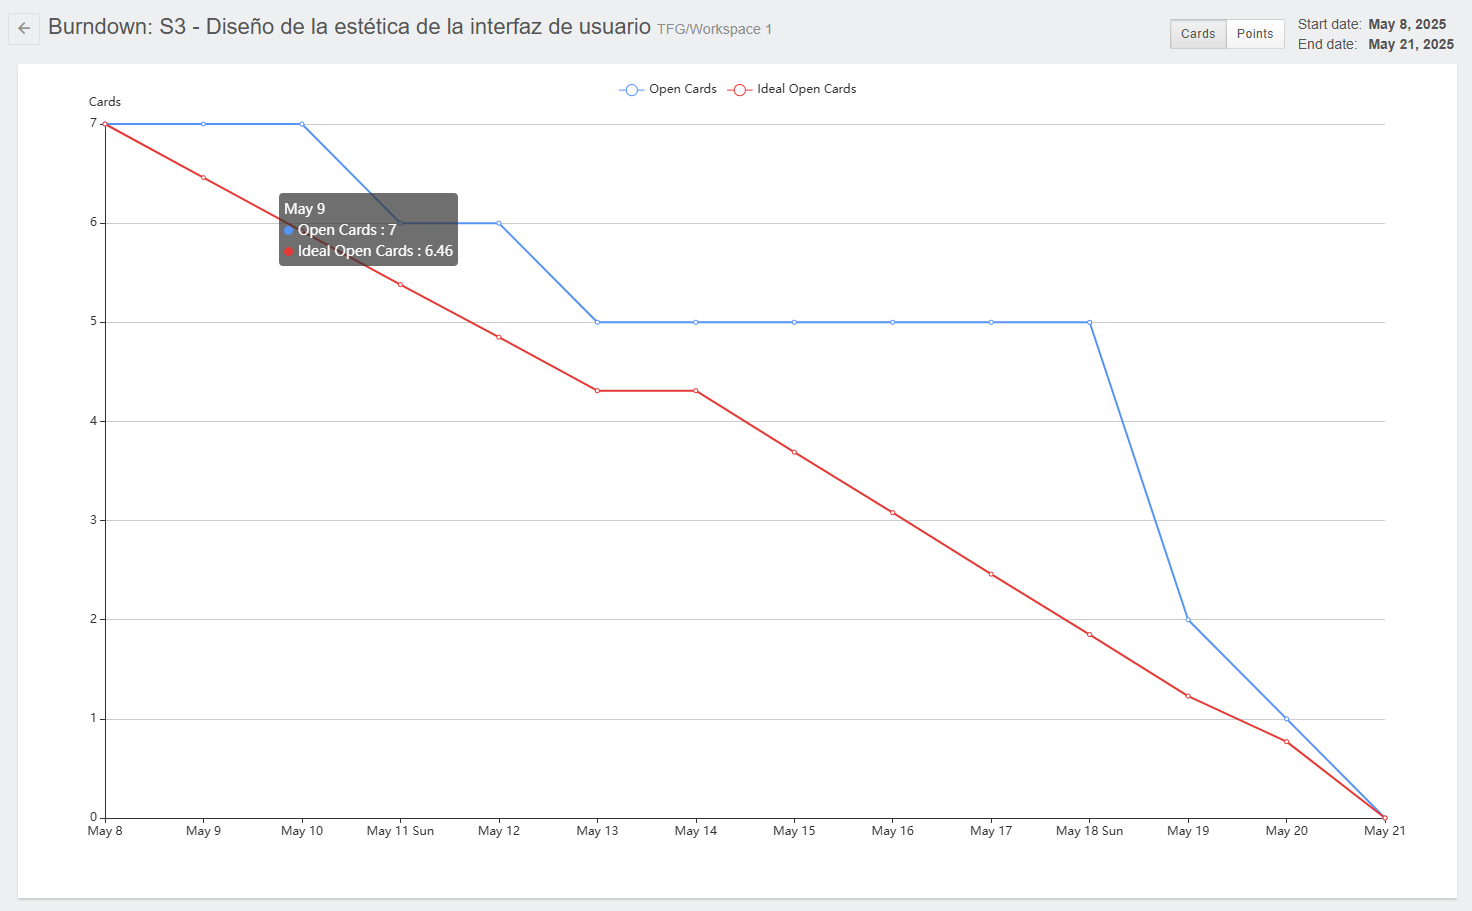
\includegraphics[width=0.8\textwidth]{img/BurndownS3.png}
\caption{Gráfico Burndown del Sprint 3}
\label{fig:BurndownS3}
\end{figure}

\begin{figure}[H]
\centering
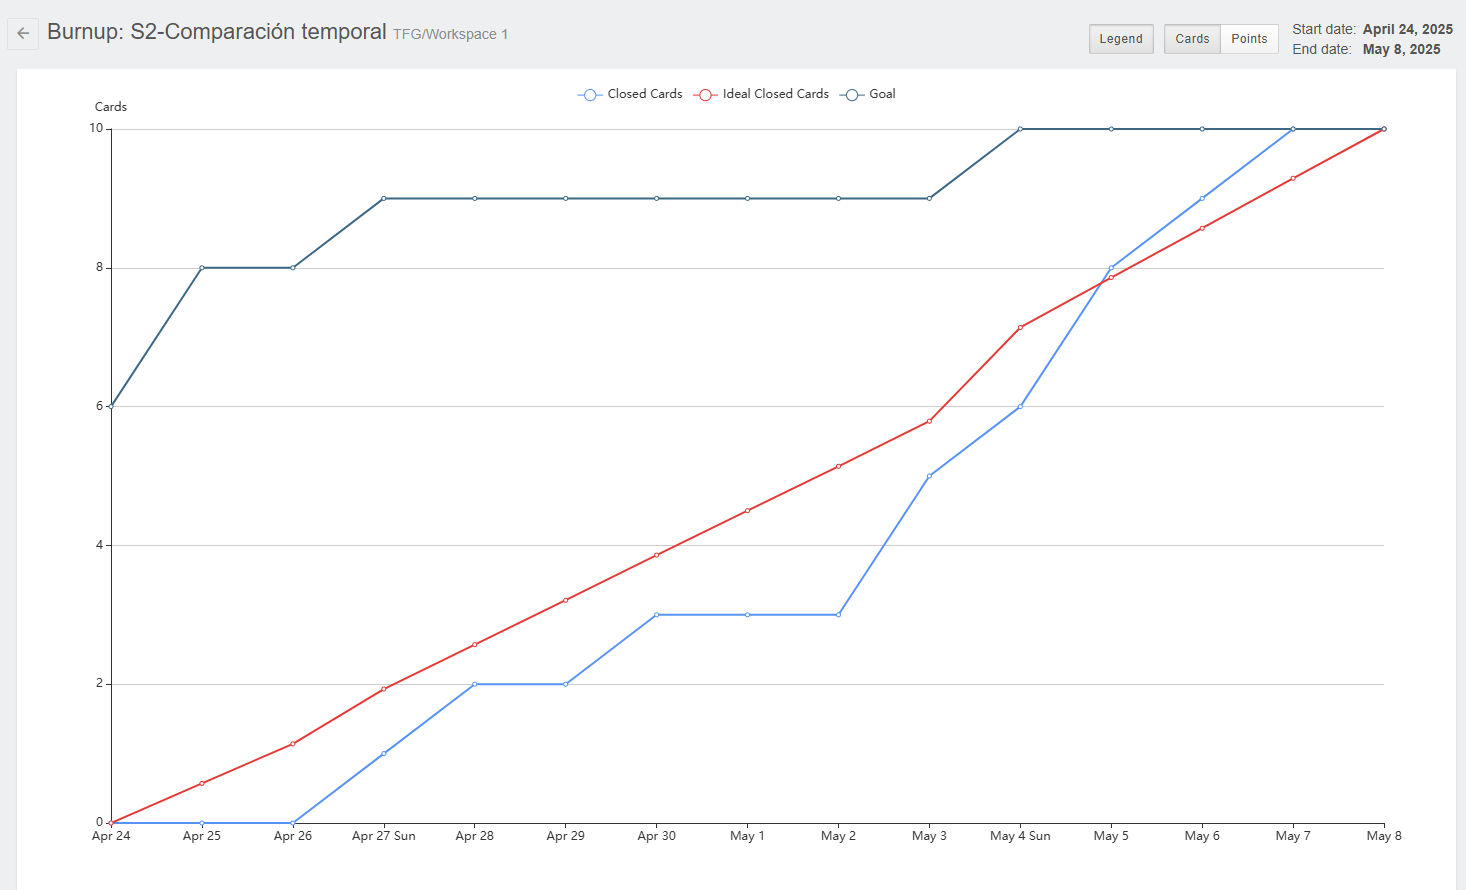
\includegraphics[width=0.8\textwidth]{img/BurnupS2.png}
\caption{Gráfico Burnup del Sprint 2}
\label{fig:BurnupS2}
\end{figure}

 A continuación se explicará cómo se ha desarrollado, por medio de \textit{sprints}, la planificación temporal del proyecto, siguiendo sus respectivas tareas y representando el flujo seguido para la creación y puesta en producción de la aplicación, así como la redacción de esta documentación del proyecto.

 Cada tarea comprendía una historia de usuario o una tarea interna de pequeño tamaño, cuya completación comprende alrededor de un día de duración. 

\begin{figure}[H]
\centering
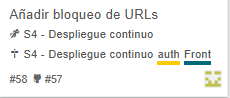
\includegraphics[width=0.8\textwidth]{img/Tarea57.png}
\caption{Ejemplo de una tarea vista en el tablero Kanban de Zube}
\label{fig:Tarea57}
\end{figure}
 
 Los \textit{sprints}, por su parte han tenido una duración media de quince días, a excepción del primero, pues requirió de varias semanas acordar las bases teóricas y objetivos principales de la aplicación.

\begin{figure}[H]
\centering
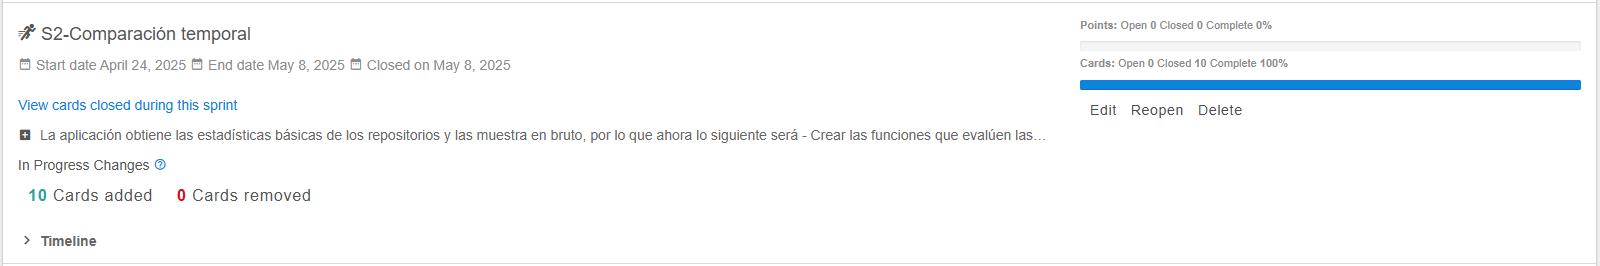
\includegraphics[width=0.8\textwidth]{img/Sprint2.png}
\caption{Ejemplo de un Sprint en Zube}
\label{fig:Sprint2}
\end{figure}

La gestión de las tareas de cada \textit{sprint} ha sido posible gracias a la herramienta del tablero KanBan, que permite gestionar de forma ágil y visual el proceso de desarrollo en el que se encuentra cada tarea. Una tarea se crea y pasa a estado \textit{ready}, preparada para ser comenzada. Una vez esta se empiece a desarrollar, la tarea pasa al estado \textit{in progress}. Una vez terminado el progreso pasará al estado de \textit{in review}, donde se revisará nuevamente el contenido de la tarea para verificar que sea correcto y esté bien implementado, y, en caso positivo, finalizar en el estado \textit{done}, como se puede ver en la siguiente imagen.

\begin{figure}[H]
\centering
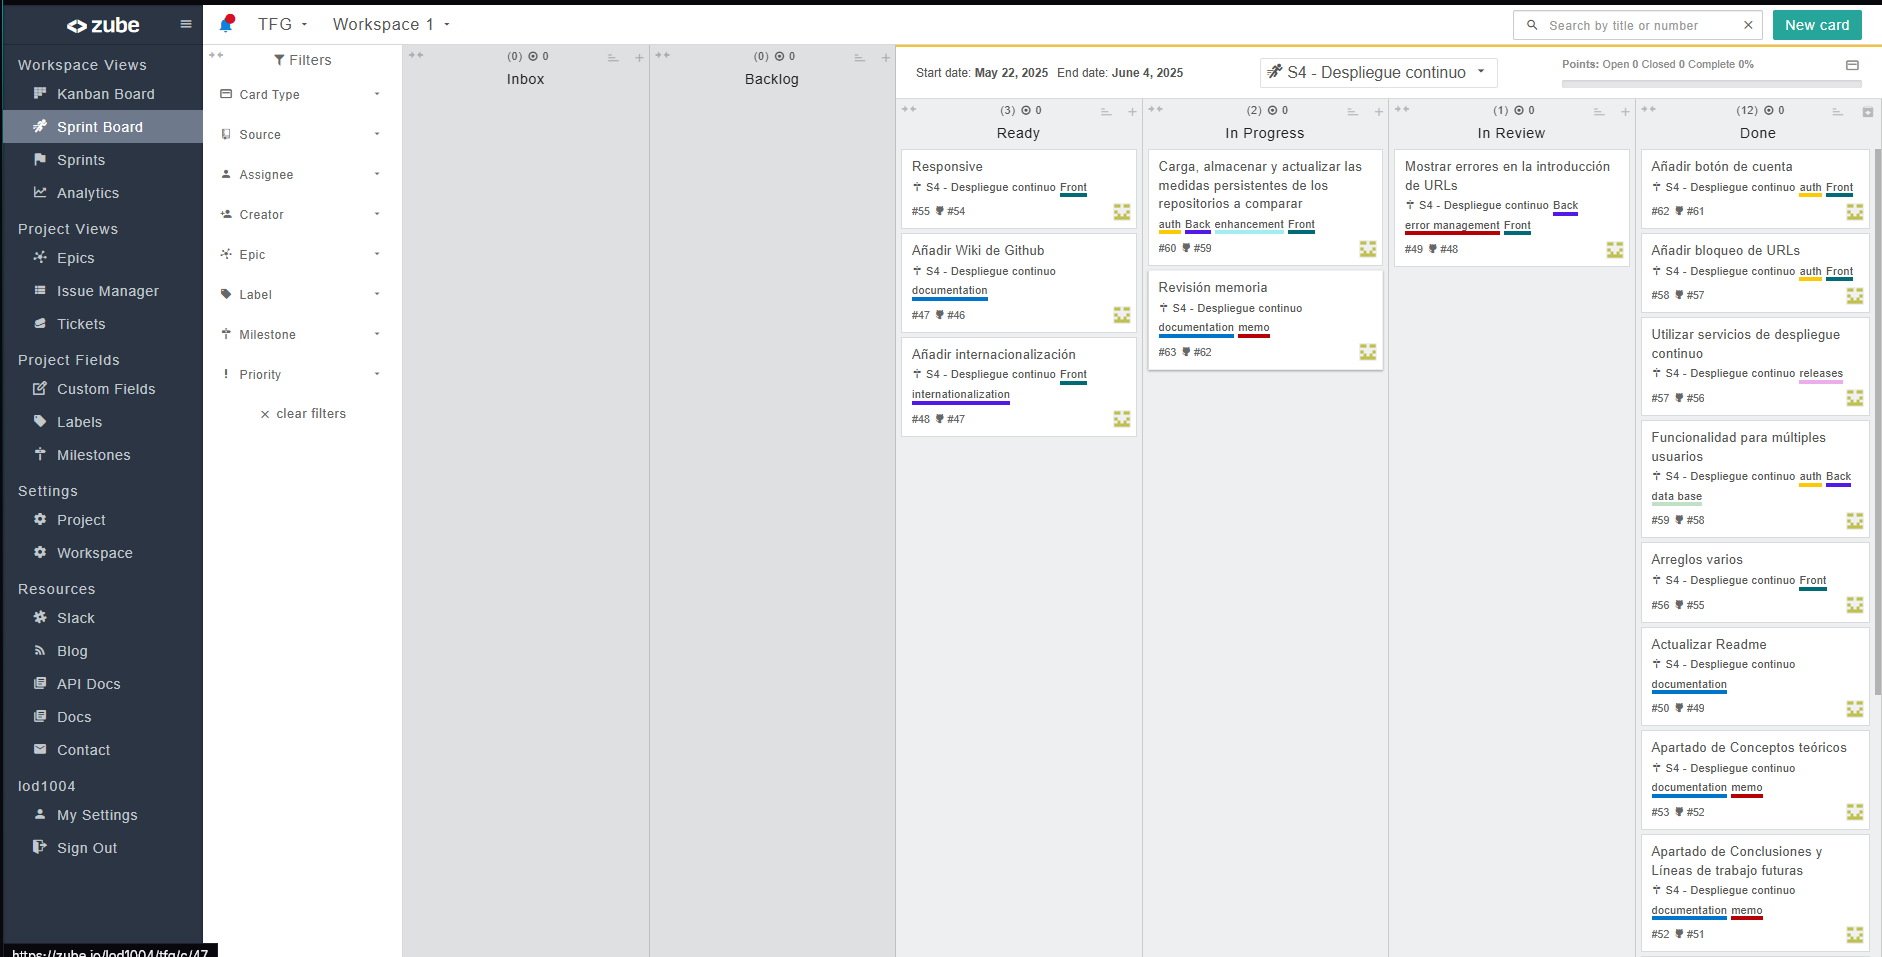
\includegraphics[width=0.8\textwidth]{img/IteracionZube.png}
\caption{Ejemplo del estado de un sprint visto en el tablero Kanban}
\label{fig:Zube}
\end{figure}

La herramienta de Zube no solo ha permitido el seguimiento del desarrollo del proyecto en tareas, sino que también ha facilitado la comunicación entre el tutor y el estudiante autor de este TFG, por medio de los comentarios disponibles en cada tarea. Al terminar cada tarea se ha puesto un comentario en la misma indicando los resultados de las actividades asociadas, en ocasiones con imágenes representativas, y el commit que los subió al repositorio del proyecto. Esto ha permitido al tutor exponer su valoración del resultado de la tarea, puntos a mejorar y/o aspectos que necesiten cambios, como se puede ver a continuación:

\begin{figure}[H]
\centering
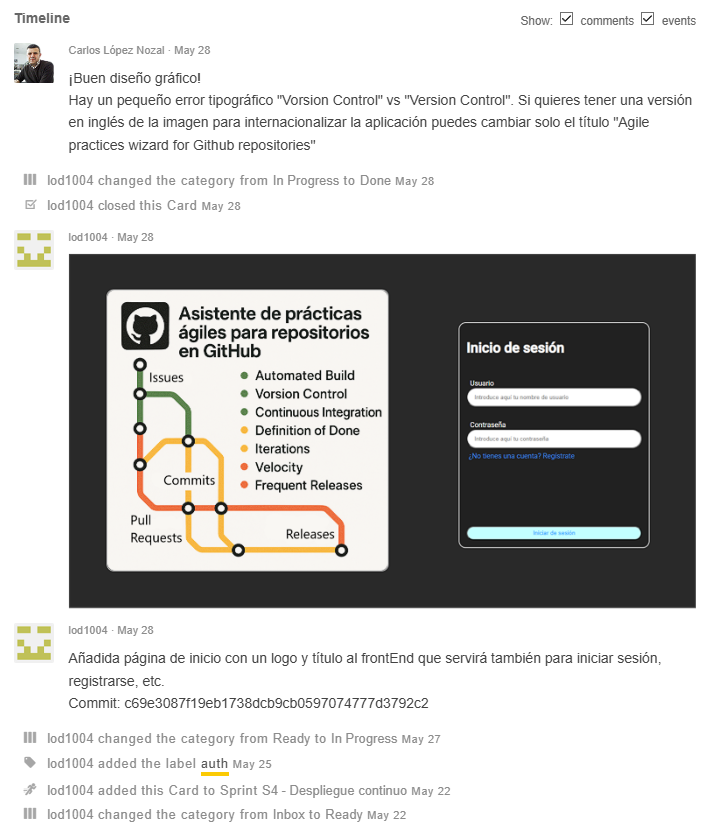
\includegraphics[width=0.8\textwidth]{img/ComentariosTareaZube.png}
\caption{Ejemplo de comentarios en Zube del tutor y alumno en una tarea del proyecto}
\label{fig:ComentariosTareaZube}
\end{figure}

\subsection{Organización en \textit{sprints}}

Para finalizar esta sección se van a desarrollar individualmente los \textit{sprints} definidos y seguidos durante el desarrollo software. Estos \textit{sprints} han sido pensados y creados durante el propio desarrollo en función del estado en el que se encontraba el proyecto, y los objetivos más adecuados que debían ser implementados en cada momento.

\subsubsection{Sprint 0 - Kick-off (1/03/2025 - 03/04/2025)}

Este sprint fue el primero y más largo de todos, pues abarcaría no solo el comienzo del desarrollo del proyecto, sino también la planificación del mismo. Se definió qué aplicación se desarrollaría, sus bases teóricas, el \textit{abstract} y los objetivos principales. Contiene las siguientes 9 tareas:

\begin{enumerate}
\item \textbf{Definir título y descripción del proyecto}: Consistió en, tras terminar de decidir los objetivos y bases del proyecto, redactar el título y descripción iniciales del mismo.
\item \textbf{Introducción del documento}: Redacción inicial del apartado de introducción de la memoria, planteando el contexto y motivación del proyecto.
\item \textbf{Revisión del resumen}: Corrección y mejora del resumen del proyecto, afinando su redacción y adecuación a los objetivos propuestos.
\item \textbf{Anexos}: Preparación de la estructura base de los anexos que acompañarán a la memoria del proyecto.
\item \textbf{Mockups}: Diseño preliminar de la interfaz de usuario para visualizar cómo se estructuraría la aplicación de forma gráfica.
\item \textbf{Definir requisitos funcionales}: Identificación de las funciones clave que debía cumplir la aplicación para alcanzar sus objetivos.
\item \textbf{Rama de pruebas}: Creación de una rama en el repositorio destinada a pruebas y experimentación durante el desarrollo que se usaría en este sprint.
\item \textbf{Estructura del front}: Primer esqueleto del frontend de la aplicación, estableciendo la organización interna de los componentes básicos.
\item \textbf{Estructura del back}: Configuración inicial del backend y definición de su arquitectura básica.
\end{enumerate}

\begin{figure}[H]
\centering
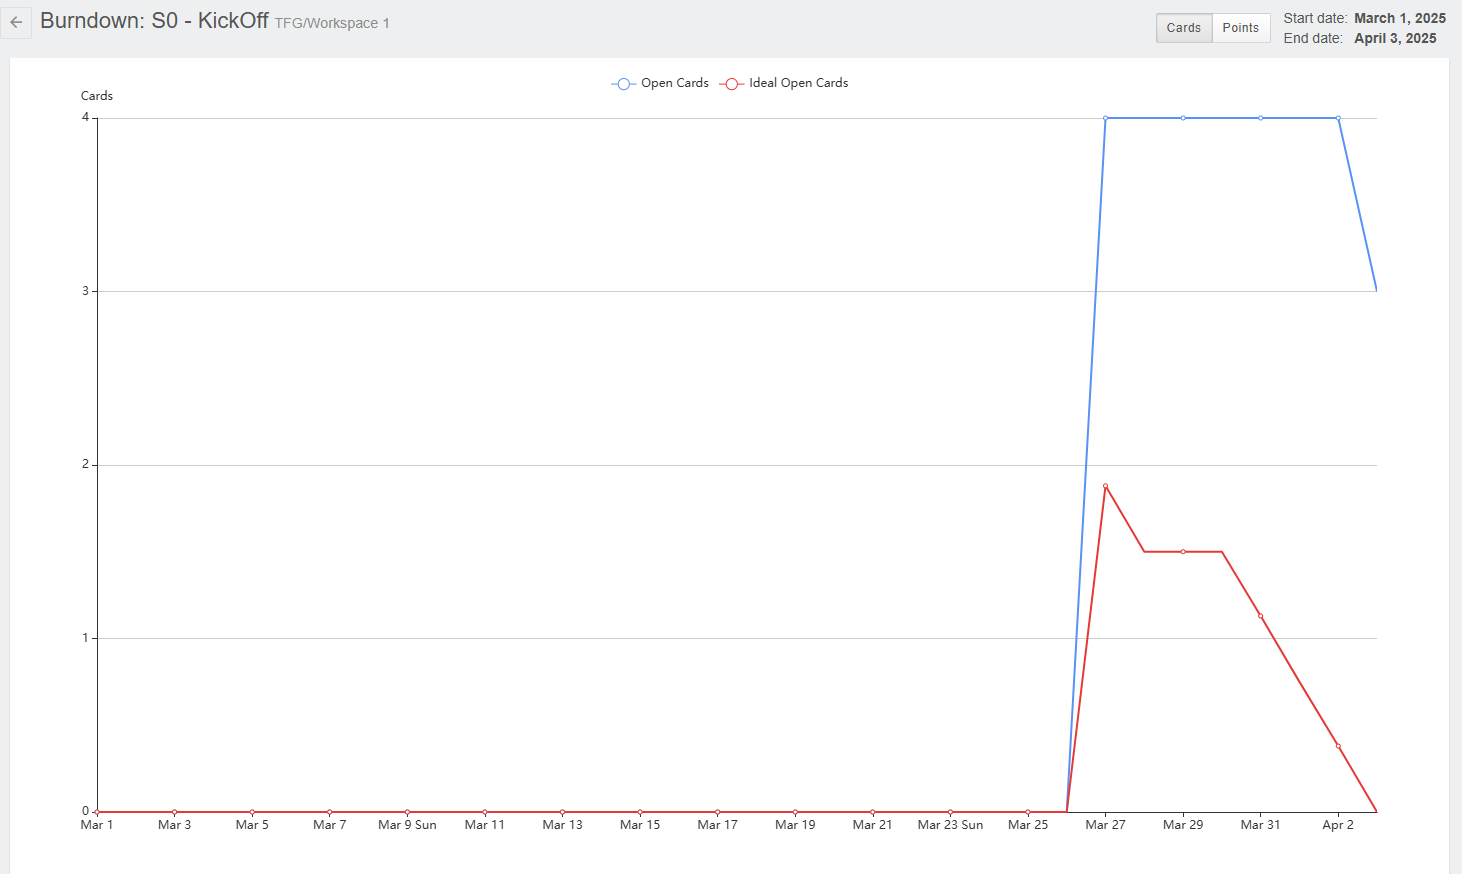
\includegraphics[width=0.8\textwidth]{img/BurndownS0.png}
\caption{Gráfico Burndown del Sprint 0}
\label{fig:BurndownS0}
\end{figure}

\begin{figure}[H]
\centering
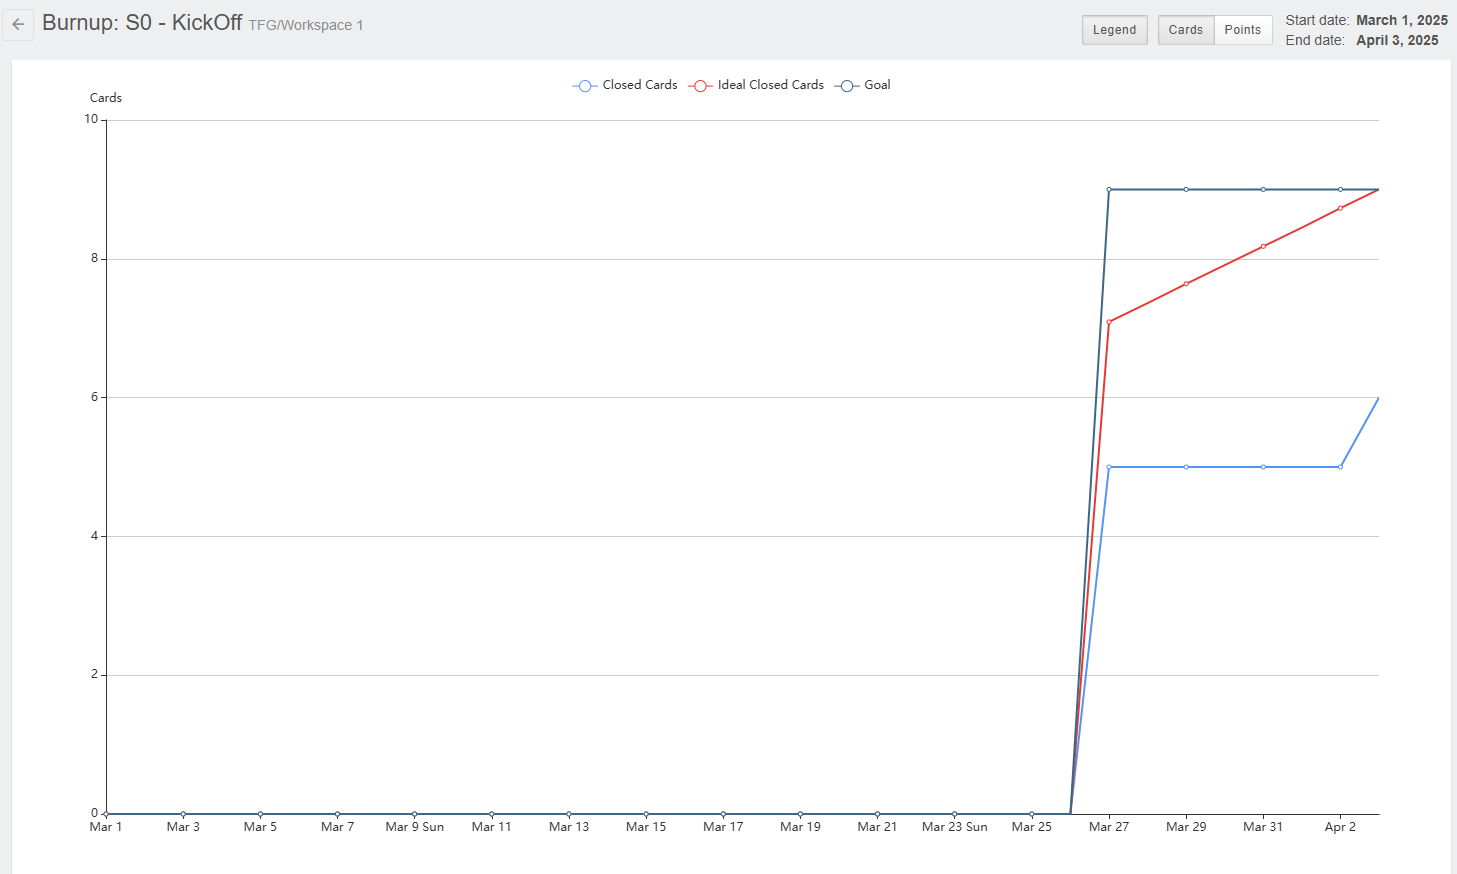
\includegraphics[width=0.8\textwidth]{img/BurnupS0.png}
\caption{Gráfico Burnup del Sprint 0}
\label{fig:BurnupS0}
\end{figure}

\subsubsection{Sprint 1 - Primer prototipo de la aplicación (8/04/2025 - 22/04/2025)}

Instaladas las herramientas básicas del proyecto y asentadas las ideas del mismo, comienza el desarrollo con un pequeño prototipo de la aplicación. Se perseguían los siguientes objetivos: conectar el backend con el frontend, definir las reglas que se evaluarán, continuar con la documentación y realizar los primeros análisis de datos.

\begin{enumerate}
\item \textbf{Conexión Front - Back}: Establecimiento de la comunicación entre el frontend y el backend.
\item \textbf{Recogida de Repositorio vía URL}: Implementación de una funcionalidad para introducir un repositorio mediante su URL.
\item \textbf{Guardar repositorio en base de datos}: Añadir la funcionalidad de almacenamiento de repositorios para su análisis posterior.
\item \textbf{Recoger número de Issues abiertas y cerradas}: Desarrollo de una métrica base para evaluar las \textit{issues} del repositorio.
\item \textbf{Mostrar número de Issues}: Visualización en la interfaz del número de \textit{issues}, como parte de las estadísticas presentadas.
\item \textbf{Evaluar mensajes de los commits}: Análisis del contenido de los mensajes de los commits para detectar buenas prácticas.
\item \textbf{Evaluar Issues en el tiempo}: Cálculo de métricas temporales sobre la evolución de los \textit{issues}.
\item \textbf{Evaluar Pull Requests}: Análisis de la actividad de las \textit{pull requests} como indicador de colaboración.
\item \textbf{Evaluar Releases}: Inclusión de información sobre las versiones liberadas del proyecto.
\item \textbf{Evaluar Acciones}: Estudio de las GitHub Actions empleadas como parte del flujo de trabajo.
\item \textbf{Definir reglas}: Redacción y codificación de las reglas de evaluación de buenas prácticas basadas en metodología ágil.
\end{enumerate}

\begin{figure}[H]
\centering
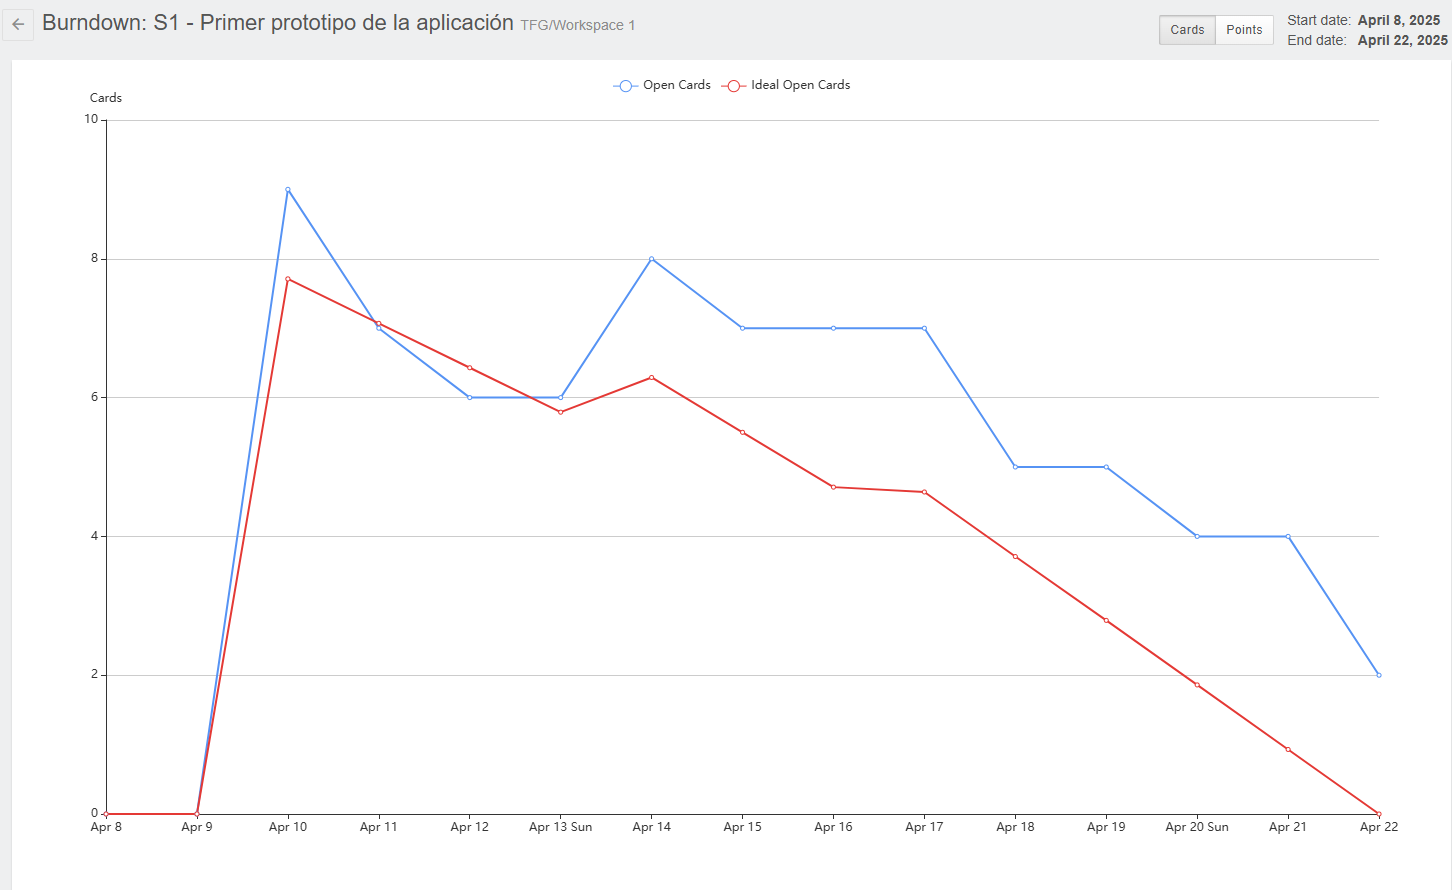
\includegraphics[width=0.8\textwidth]{img/BurndownS1.png}
\caption{Gráfico Burndown del Sprint 1}
\label{fig:BurndownS1}
\end{figure}

\begin{figure}[H]
\centering
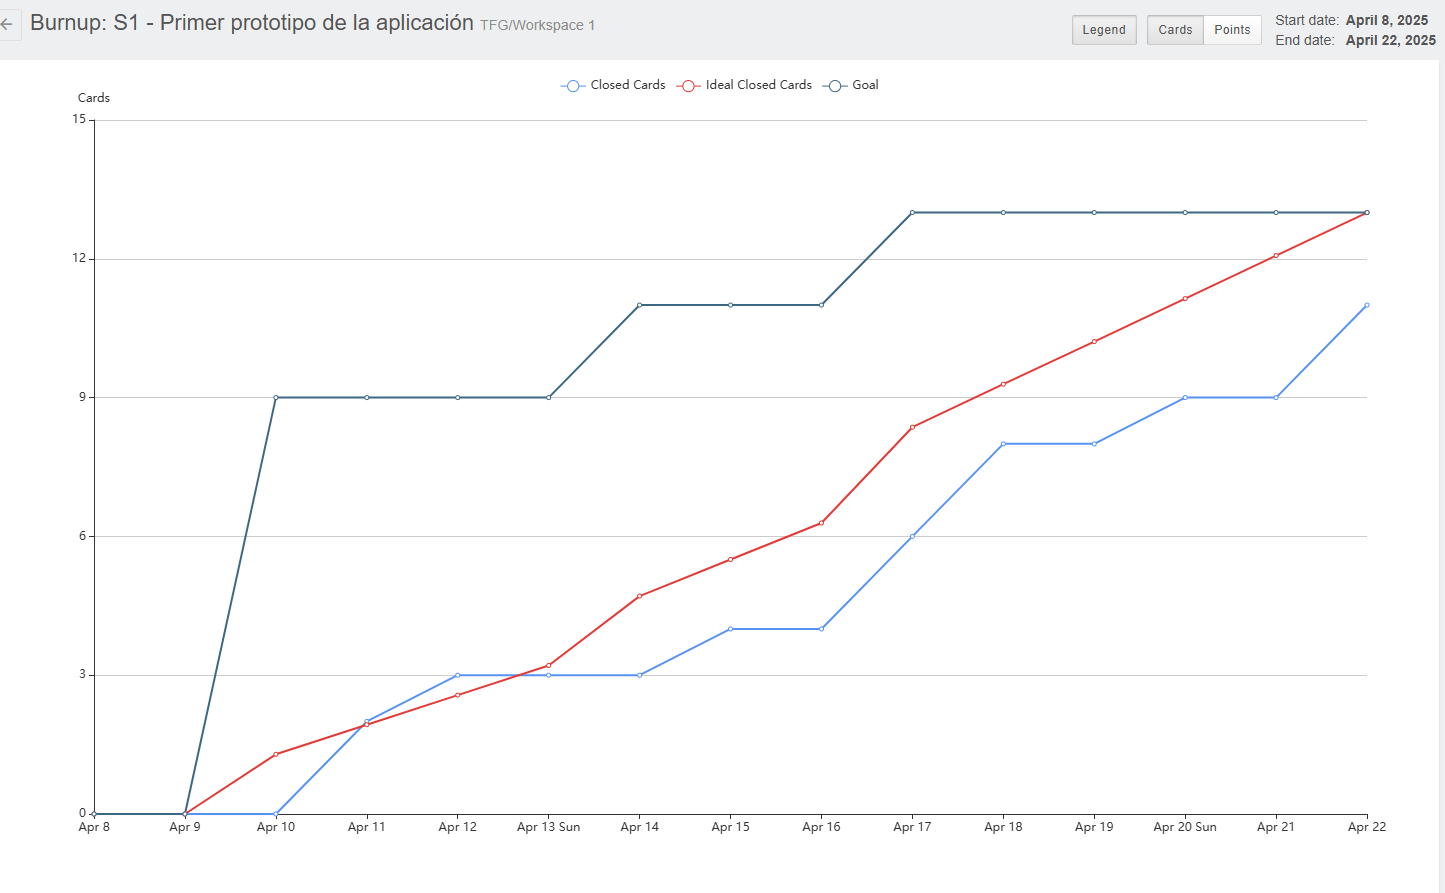
\includegraphics[width=0.8\textwidth]{img/BurnupS1.png}
\caption{Gráfico Burnup del Sprint 1}
\label{fig:BurnupS1}
\end{figure}

\subsubsection{Sprint 2 - Comparación temporal (24/04/2025 - 08/05/2025)}

La aplicación ya obtiene estadísticas básicas. En este sprint se centró en implementar una comparación temporal entre repositorios, añadir control de errores y documentar la evolución temporal de los proyectos.

\begin{enumerate}
\item \textbf{Crear funciones de las reglas}: Implementación concreta de las funciones para evaluar las reglas definidas.
\item \textbf{Mostrar cumplimiento de reglas}: Inclusión en el frontend de indicadores que muestran si se cumplen las reglas.
\item \textbf{Extraer intervalos de tiempo del repositorio}: Implementar la funcionalidad de los intervalos de tiempo para comparar la actividad del repositorio.
\item \textbf{Selección de intervalos de tiempo}: Interfaz para que el usuario pueda seleccionar intervalos de tiempo a usar en el análisis.
\item \textbf{Añadir estadísticas temporales}: Implementación de métricas que reflejen la evolución cada cierto número de días.
\item \textbf{Añadir estadísticas restantes}: Inclusión de estadísticas que aún no habían sido implementadas.
\item \textbf{Estadísticas de participantes}: Incorporación de datos sobre los miembros del repositorio.
\item \textbf{Ordenar Base de datos}: Refactorización y optimización de la estructura de almacenamiento de repositorios y medidas de calidad de proceso.
\item \textbf{Añadir control de errores}: Añadir gestión de errores para situaciones como problemas de red o repositorios no válidos.
\item \textbf{Documentar sobre la evolución de proyectos en el tiempo}: Redacción teórica en la memoria sobre las fases de un proyecto ágil.
\end{enumerate}

\begin{figure}[H]
\centering
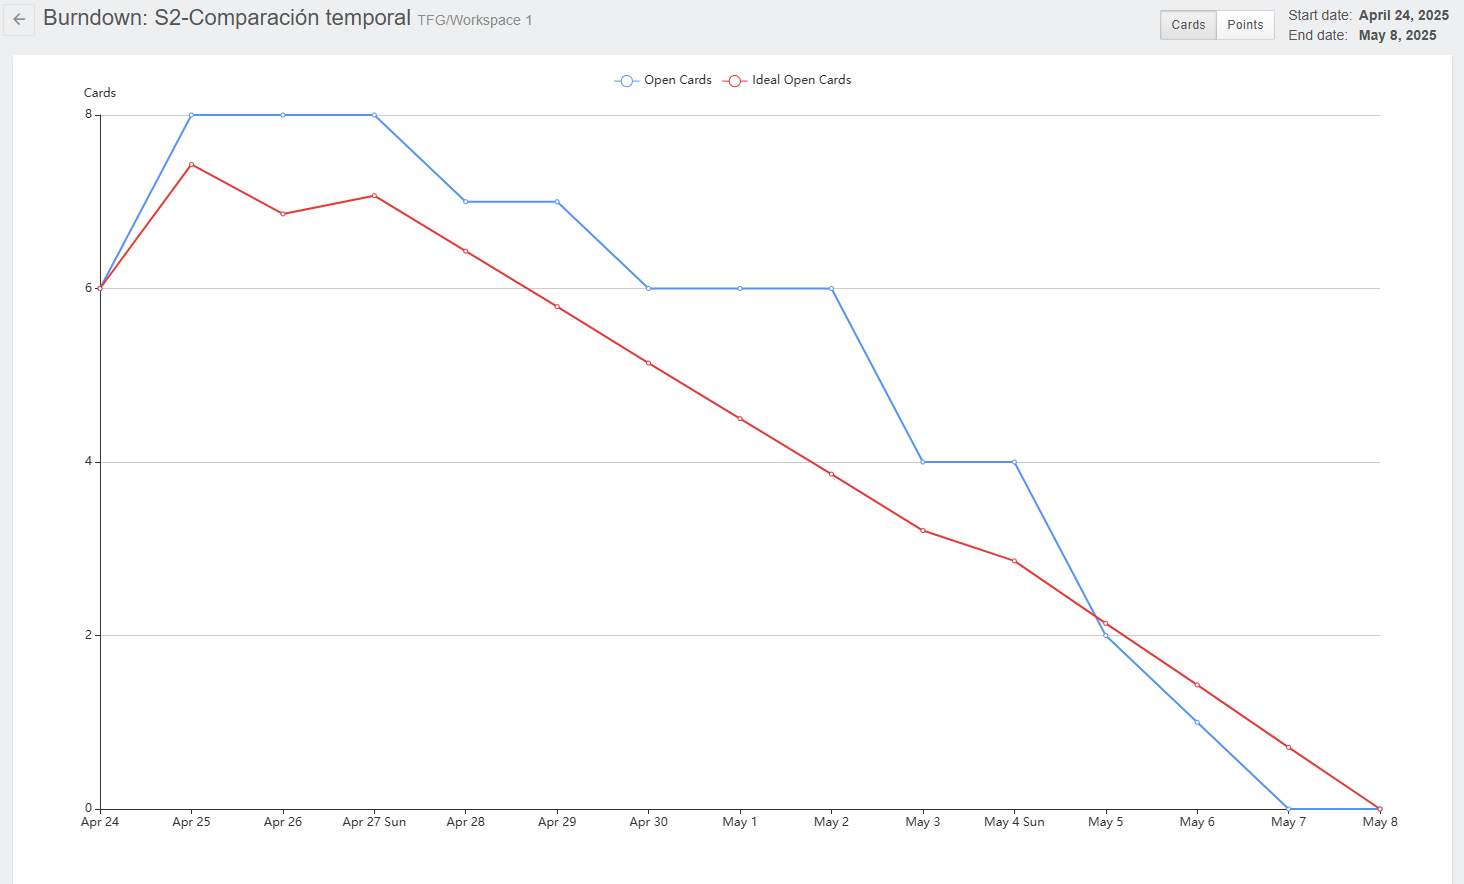
\includegraphics[width=0.8\textwidth]{img/BurndownS2.png}
\caption{Gráfico Burndown del Sprint 2}
\label{fig:BurndownS2}
\end{figure}

\begin{figure}[H]
\centering
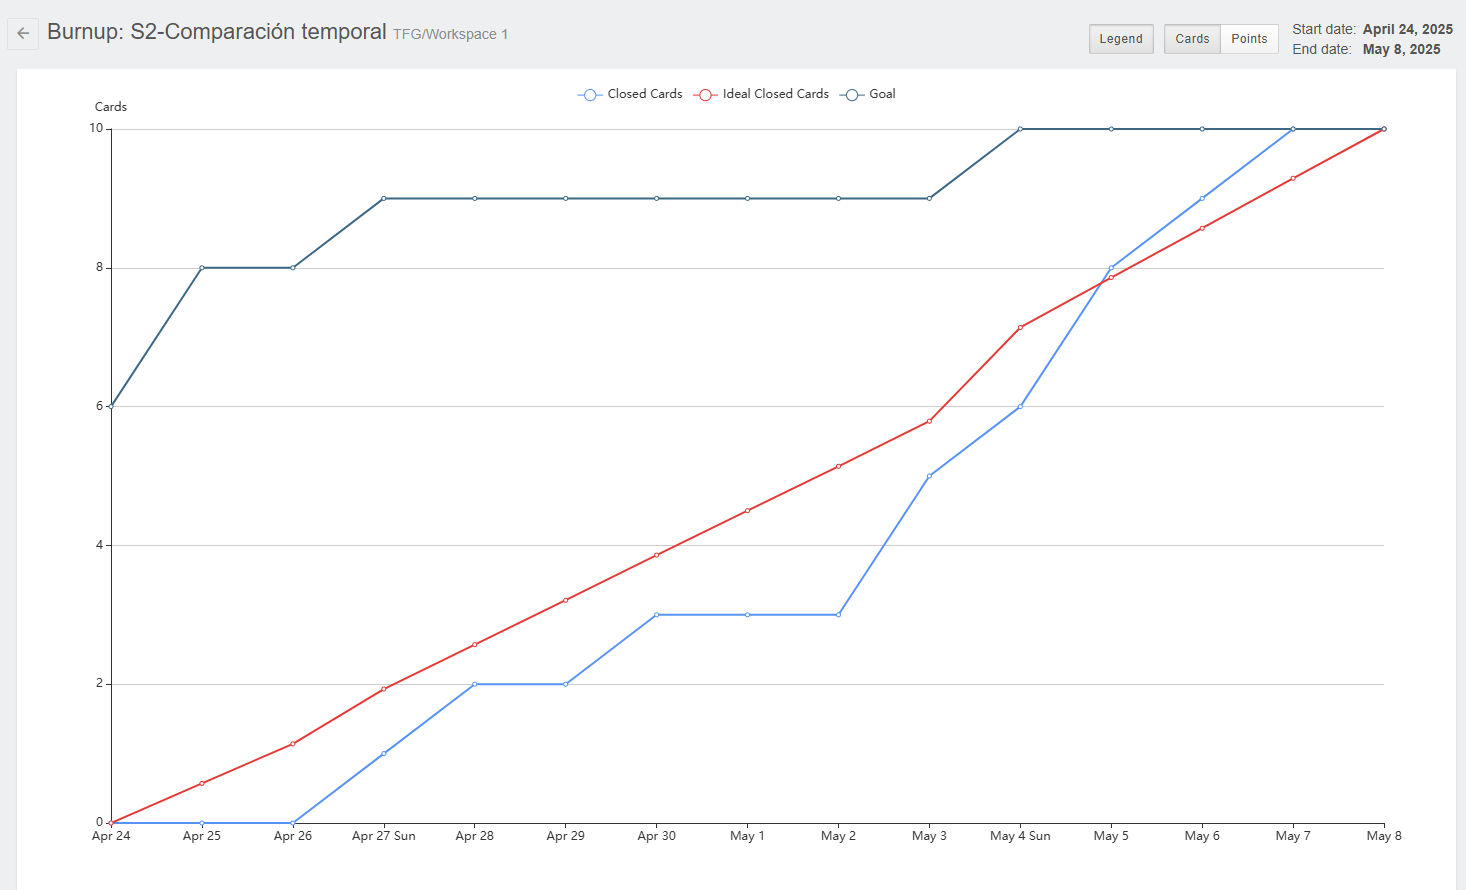
\includegraphics[width=0.8\textwidth]{img/BurnupS2.png}
\caption{Gráfico Burnup del Sprint 2}
\label{fig:BurnupS2}
\end{figure}

\subsubsection{Sprint 3 - Diseño de la estética de la interfaz de usuario (08/05/2025 - 21/05/2025)}

Con una versión funcional disponible, se procedió a mejorar la experiencia de usuario y seguir avanzando en la documentación del proyecto.

\begin{enumerate}
\item \textbf{Maquetación del FrontEnd}: Rediseño visual del frontend para mejorar la experiencia y estética.
\item \textbf{Nuevas estadísticas y revisión}: Mejora de algunas métricas, añadido de alguans nuevasy validación de los resultados obtenidos.
\item \textbf{Añadir Spinner}: Mejora visual mediante un componente que indica la carga de información.
\item \textbf{Implementar logs}: Sistema de registro de eventos para facilitar el mantenimiento.
\item \textbf{Información sobre resultados de las reglas}: Mostrar explicaciones detalladas de cada regla y su resultado.
\item \textbf{Apartado de "Trabajos Relacionados"}: Redacción del apartado que contextualiza el trabajo con investigaciones previas.
\item \textbf{Apartado de "Aspectos relevantes del desarrollo"}: Inclusión en la memoria de las decisiones clave durante el desarrollo.
\item \textbf{Apartado de "Objetivos del proyecto"}: Definición clara de los objetivos concretos que se querían alcanzar.
\item \textbf{Apartado de "Técnicas y herramientas"}: Descripción de las herramientas usadas y su justificación.
\item \textbf{Primera Release del proyecto}: Publicación de la primera versión oficial v0.1.0 de la aplicación.
\end{enumerate}

\begin{figure}[H]
\centering
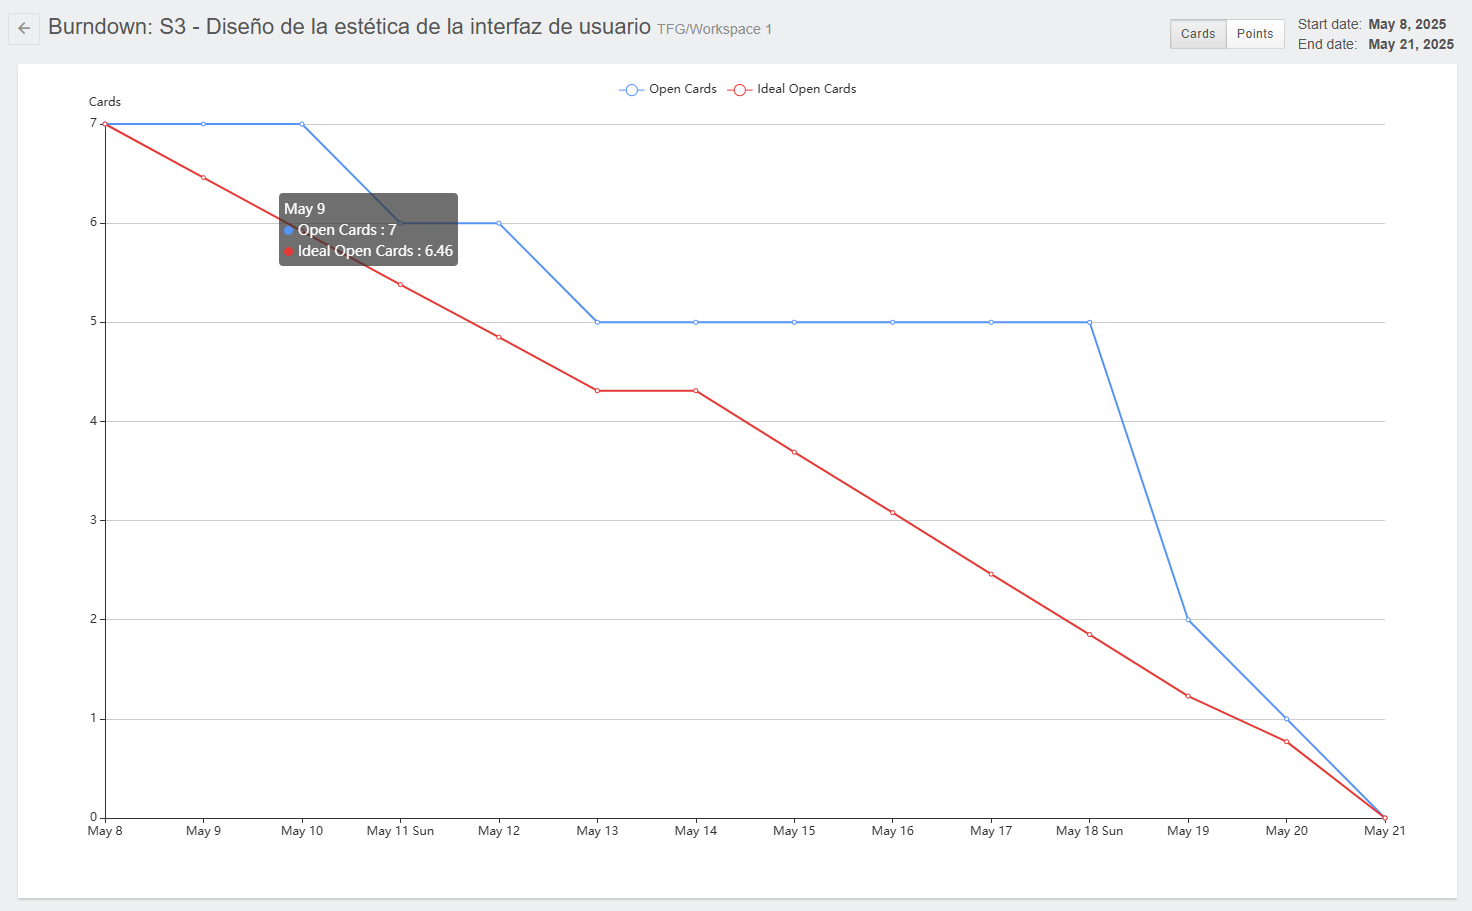
\includegraphics[width=0.8\textwidth]{img/BurndownS3.png}
\caption{Gráfico Burndown del Sprint 3}
\label{fig:BurndownS3}
\end{figure}

\begin{figure}[H]
\centering
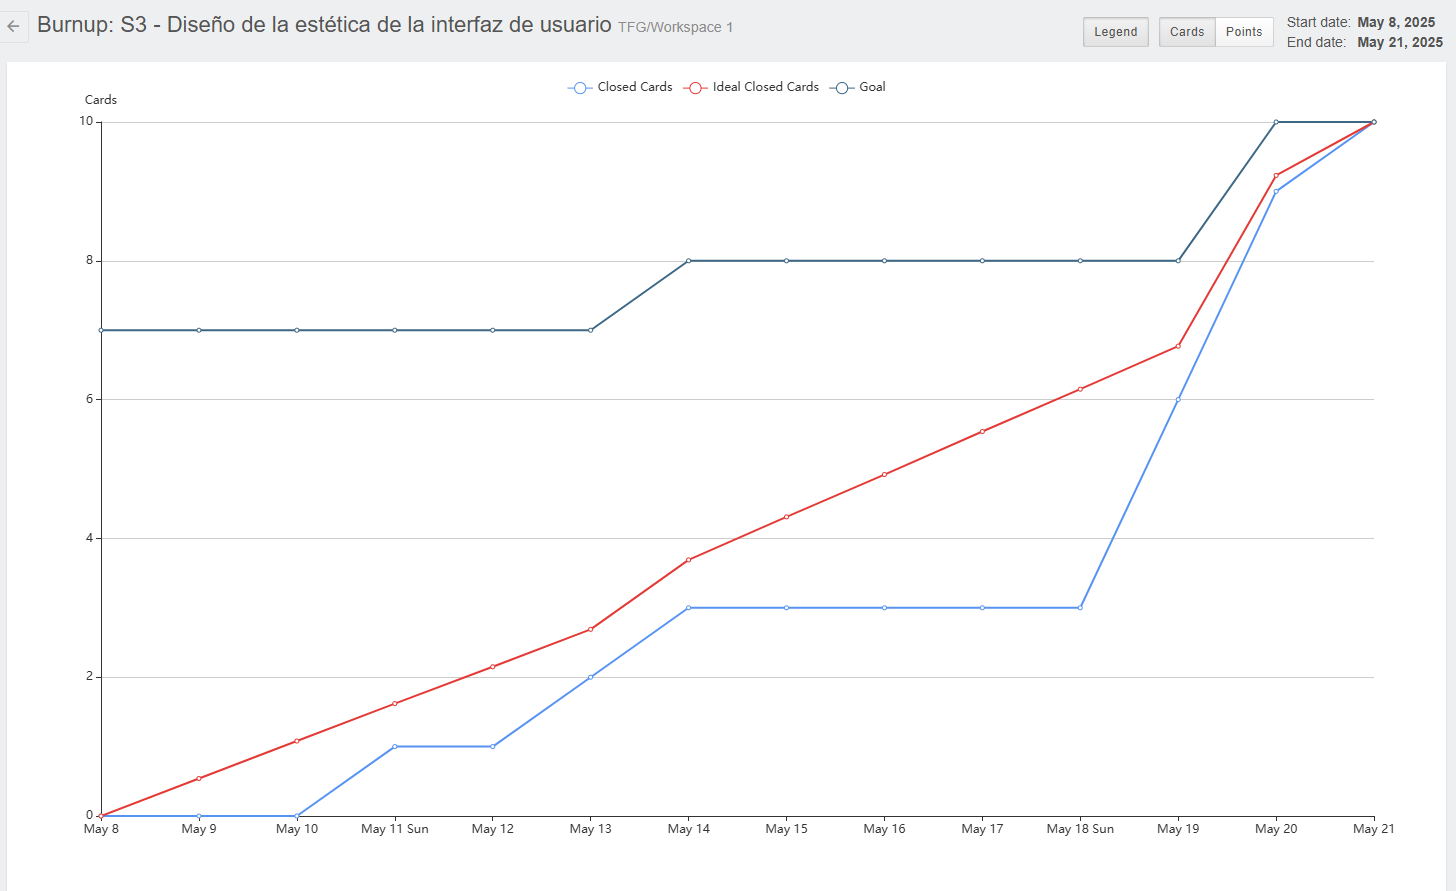
\includegraphics[width=0.8\textwidth]{img/BurnupS3.png}
\caption{Gráfico Burnup del Sprint 3}
\label{fig:BurnupS3}
\end{figure}

\subsubsection{Sprint 4 - Despliegue continuo (22/05/2025 - 04/06/2025)}

En este último sprint se trabajó en el despliegue de la aplicación, correcciones finales, soporte para múltiples usuarios y finalización de la memoria.

\begin{enumerate}
\item \textbf{Utilizar servicios de despliegue continuo}: Implementación de un flujo de despliegue automático tras cada actualización.
\item \textbf{Responsive}: Adaptación de la interfaz a distintos tamaños de pantalla.
\item \textbf{Mostrar errores en la introducción de URLs}: Validación del input del usuario para evitar URLs no válidas.
\item \textbf{Añadir internacionalización}: Soporte para diferentes idiomas en la interfaz de usuario.
\item \textbf{Añadir página de inicio}: Creación de una landing page para la aplicación que serviría como formulario de login.
\item \textbf{Cambiar título y nomenclaturas}: Revisión de nombres de variables y componentes para mayor claridad.
\item \textbf{Actualizar Readme}: Actualización de la documentación principal del repositorio con instrucciones claras.
\item \textbf{Añadir Wiki de Github}: Creación de una wiki complementaria al README para documentar el uso.
\item \textbf{Añadir usuarios y login}: Implementación básica de autenticación de usuarios.
\item \textbf{Funcionalidad para múltiples usuarios}: Adaptación del backend para permitir análisis separados por usuario.
\item \textbf{Añadir botón de cuenta}: Crear un botón de apertura del menú de usuario.
\item \textbf{Revisión memoria}: Revisión general del contenido escrito de la memoria.
\item \textbf{PDF completo de la memoria}: Generación del documento final completo en formato PDF.
\item \textbf{Apartado de Conclusiones y Líneas de trabajo futuras}: Reflexión final sobre el proyecto y posibles continuaciones en la memoria.
\item \textbf{Apartado A de los anexos}: Redacción del apartado A de los anexos.
\item \textbf{Revisión del apartado B de los anexos}: Revisión del apartado B de los anexos.
\item \textbf{Apartado C de los anexos}: Redacción del apartado C de los anexos.
\item \textbf{Apartado D de los anexos}: Redacción del apartado D de los anexos.
\item \textbf{Apartado E de los anexos}: Redacción del apartado E de los anexos.
\item \textbf{Apartado F de los anexos}: Redacción del apartado F de los anexos.
\item \textbf{Anexos (finales)}: Inclusión de todos los anexos restantes con los elementos complementarios.
\item \textbf{Test eficiencia v.0.2.0}: Evaluación de la eficiencia del sistema tras la última versión.
\item \textbf{Arreglos varios}: Correcciones menores y ajustes visuales o funcionales.
\end{enumerate}

\begin{figure}[H]
\centering
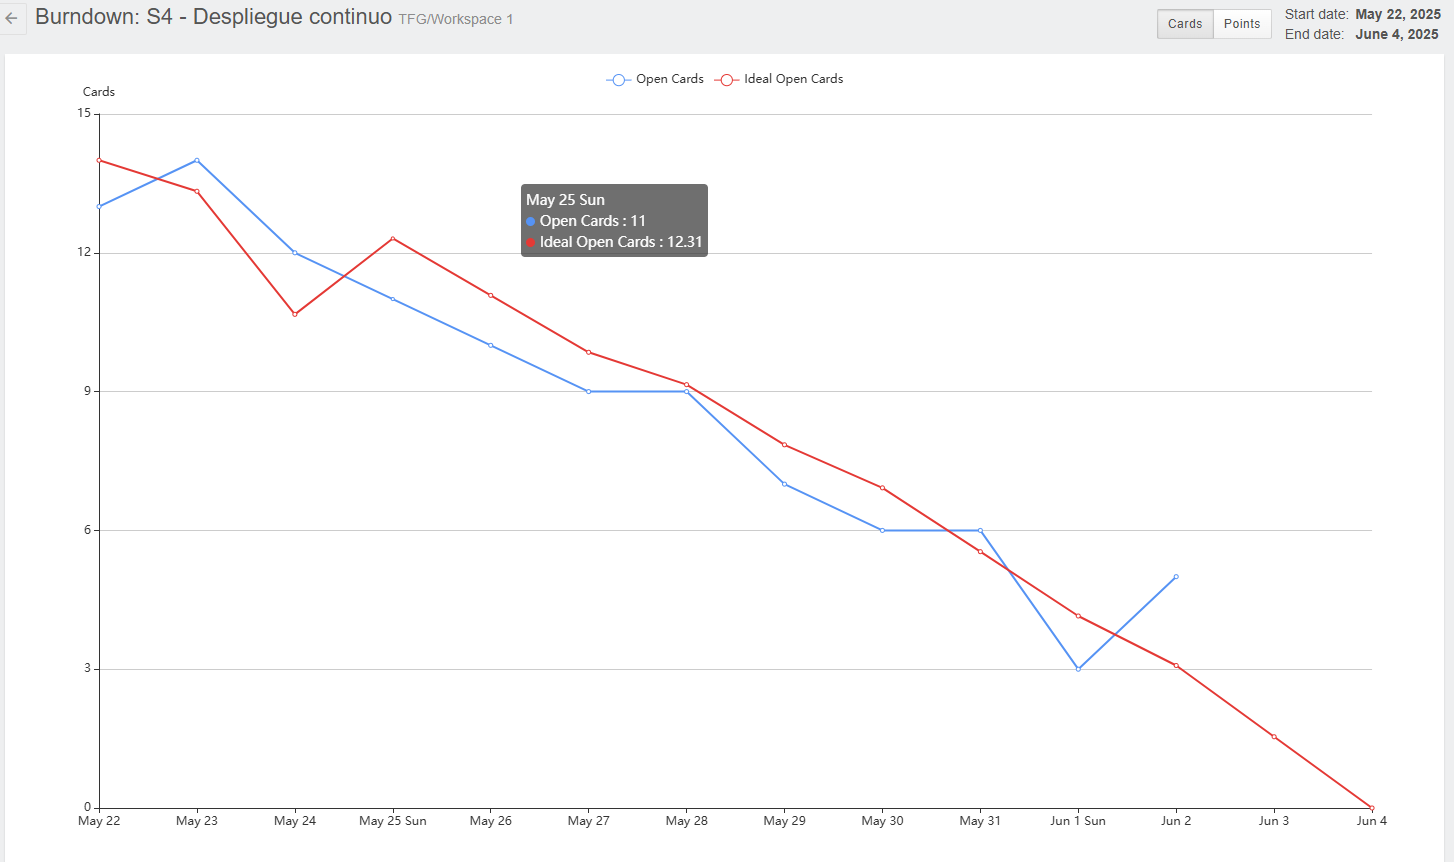
\includegraphics[width=0.8\textwidth]{img/BurndownS4.png}
\caption{Gráfico Burndown del Sprint 4}
\label{fig:BurndownS4}
\end{figure}

\begin{figure}[H]
\centering
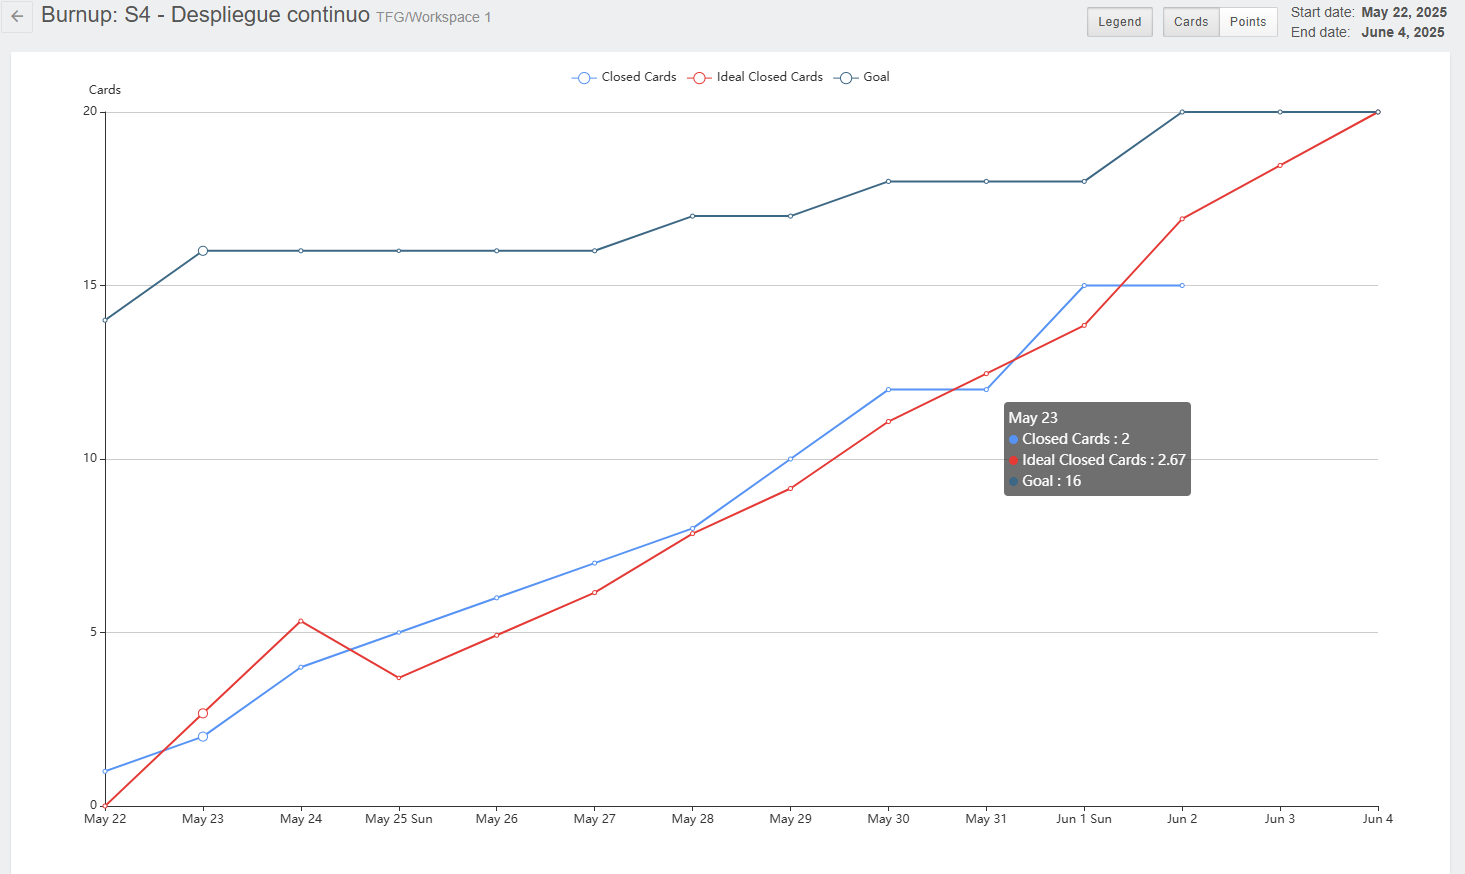
\includegraphics[width=0.8\textwidth]{img/BurnupS4.png}
\caption{Gráfico Burnup del Sprint 4}
\label{fig:BurnupS4}
\end{figure}

\section{Estudio de viabilidad}

Este apartado recoge un análisis detallado sobre la viabilidad del proyecto desde una doble perspectiva: económica y legal. Se examinan los recursos necesarios para el desarrollo de la aplicación web \textbf{Asistente de prácticas ágiles para repositorios en GitHub} en equipos de desarrollo que utilizan GitHub, así como los requisitos y restricciones legales que podrían condicionar su puesta en marcha. Dado su enfoque académico, automatizado y extensible, el proyecto se plantea como una herramienta útil tanto para entornos académicos como profesionales, y su desarrollo es asumido por un único responsable técnico.

\subsection{Viabilidad económica}

\subsubsection{Costes de personal}

El desarrollo ha sido asumido por una sola persona con perfil de estudiante de ingeniería informática. De acuerdo con el XVIII Convenio Colectivo Estatal de Empresas de Consultoría y Tecnologías de la Información \cite{boe2023_consultoria}, se estima un coste bruto mensual en torno a 2.000 €. Para el desarrollo completo del proyecto se contemplan hasta 4 meses de trabajo.

\tablaSmallSinColores
{Costes de \textit{personal}}
{lc}
{costes-personal}
{%
	\textbf{Concepto} & \textbf{Coste} \\
}
{%
	Salario mensual & 1.500€ \\
	Seguridad Social y retenciones & 500€ \\
	\midrule
	\textbf{Total 4 meses} & \textbf{8.000€} \\
}

\subsubsection{Coste de hardware}

Se presupone la utilización de un equipo de sobremesa ya disponible con prestaciones suficientes para ejecutar herramientas de desarrollo, e instalar aplicaciones y herramientas de programación y puesta en producción, así como entornos de inferencia local. A efectos contables, se considera una amortización del equipo a 3 años.

\tablaSmallSinColores
{Costes de \textit{hardware}}
{lcc}
{costes-hardware}
{%
	\textbf{Concepto} & \textbf{Coste} & \textbf{Coste amortizado} \\
}
{%
	Ordenador de desarrollo & 500€ & 113€ \\
	Teléfono móvil para pruebas para interfaces responsive & 250€ & 83€ \\
	\midrule
	\textbf{Total} & \textbf{750€} & \textbf{196€} \\
}

\subsubsection{Coste de conectividad}

El uso continuo de internet es fundamental, tanto para descargar dependencias como para utilizar APIs de inferencia o conectarse a servicios de terceros como GitHub, Vercel o Render. Se estima un coste medio mensual de 35€.

\begin{itemize}
	\item \textbf{Total en conectividad (4 meses):} 140€
\end{itemize}

\subsubsection{Coste de software}

Todo el software utilizado en el desarrollo es de código abierto o con licencias gratuitas para su uso individual: Visual Studio Code, GitHub, Vercel (usando entornos públicos gratuitos) y React. El sistema operativo empleado es Windows 10 Home, de un coste de alrededor de 10 euros y ampliamente compatible con las herramientas mencionadas.

\textbf{Coste estimado: 10€}

\subsubsection{Auditoría y supervisión académica}

Se reserva un coste temporal asociado al seguimiento del proyecto por parte del tutor, que incluye la corrección del código, revisión de entregables y reuniones de orientación técnica.

\tablaSmallSinColores
{Costes totales del asistente inteligente para prácticas ágiles}
{lc}
{costes-totales}
{%
	\textbf{Concepto} & \textbf{Coste} \\
}
{%
	Mano de obra & 8.000€ \\
	Hardware amortizado & 196€ \\
	Conectividad & 140€ \\
	Software Windows 10 & 10€ \\
	Revisión académica & 550€ \\
	\midrule
	\textbf{Total} & \textbf{9.306€} \\
}

\subsubsection{Sostenibilidad económica del proyecto}

Una vez completado el desarrollo inicial, el coste de mantenimiento es bajo, especialmente si se utilizan modelos locales. La monetización del asistente podría basarse en:

\begin{itemize}
	\item \textbf{Licencia freemium:} acceso básico gratuito y funciones avanzadas bajo suscripción.
	\item \textbf{Integración en GitHub Marketplace:} cobro por instalación en organizaciones.
	\item \textbf{Modelo educativo:} cesión gratuita a universidades con apoyo institucional.
\end{itemize}

\subsection{Viabilidad legal}

\subsubsection{Licencias del software utilizado}

Se ha garantizado el uso exclusivo de herramientas de código abierto o con licencias permissivas  Esto incluye tanto las librerías públicas usadas en el frontend y el backend como herramientas de despliegue continuo como Vercel o React

\begin{itemize}
	\item Librearías de Angular y Node-js.
	\item Integraciones continuas con GitHub, Vercel y React.
\end{itemize}

\subsubsection{Términos de uso de las APIs de terceros}

Al utilizar servicios de inferencia por API (En este caso GitHub API) deben respetarse las políticas de uso responsable, límites de almacenamiento de datos y uso no comercial sin licencia explícita.

\textbf{Requisitos:}

\begin{itemize}
	\item Consentimiento del usuario en el tratamiento de repositorios.
	\item Prohibición del reentrenamiento sobre inputs sin autorización.
\end{itemize}

\subsubsection{Protección de datos}

En caso de desplegar el asistente en organizaciones reales, será necesario cumplir con la normativa de protección de datos como el RGPD:

\begin{itemize}
	\item Anonimización de inputs del usuario.
	\item Consentimiento explícito para recoger métricas.
	\item Política de privacidad visible.
\end{itemize}

\subsubsection{Restricciones de publicación}

Si el asistente se publica en plataformas como GitHub Marketplace o se distribuye como SaaS, deberá incluir:

\begin{itemize}
	\item Condiciones de uso claras.
	\item Política de privacidad.
	\item Declaración de uso de APIs externas.
\end{itemize}

\subsubsection{Checklist legal}

\begin{enumerate}
	\item Verificación de licencias de todas las librerías.
	\item Inclusión de política de privacidad si se recoge algún dato.
	\item Revisión de los términos de cada API externa usada.
	\item Consentimiento de usuario informado en contextos reales.
	\item Uso responsable de la inferencia (sin outputs automatizados sin revisión humana en contextos críticos).
\end{enumerate}

Cumpliendo estas condiciones, la legalidad de la aplicación está asegurada y no representa impedimentos para su desarrollo ni distribución futura.
\apendice{Especificación de Requisitos}

\section{Introducción}

Este apéndice recoge los requisitos funcionales de la aplicación propuesta en este proyecto para evaluar la adopción de prácticas ágiles en repositorios de GitHub utilizados por estudiantes para realizar diversos trabajos como, por ejemplo, Trabajos de Fin de Grado (TFG). Se incluyen los casos de uso posibles que podrá tener un usuario de la aplicación desarrollada, junto a tablas y diagramas que ayuden a comprender los mismos. Los casos de uso comprenderán cierto número de requisitos funcionales y no funcionales, listados y explicados más adelante en este apartado para especificar claramente todas las formas que tiene el usuario de interactuar con el software propuesto. Además se incluirá el listado de objetivos generales del proyecto para ayudar a contextualizar tanto los casos de uso como los requisitos funcionales.

\section{Objetivos generales}
La visión general de este proyecto abarca los objetivos descritos a continuación:

\begin{itemize}

\item \textbf{Análisis de métricas de calidad de proceso de software de los repositorios}: La aplicación web analiza detalladamente todas las métricas de calidad de proceso y características que pueden resultar útiles de un repositorio durante el proceso de desarrollo de software.

\item \textbf{Ajuste temporal del análisis}: Consiste en la posibilidad de ajustar distintos parámetros temporales del análisis para elegir en qué etapas del desarrollo se analizarán los repositorios.

\item \textbf{Comparación de las métricas de calidad de proceso obtenidas de los repositorios de referencia}: La aplicación es capaz de, dadas todas las medidas de calidad de proceso de los repositorios que el usuario ha elegido como referencia, compararlas para ofrecer al usuario una visualización clara de los diferentes valores de estas medidas en los distintos repositorios.

\item \textbf{Prácticas ágiles y medidas de repositorios}: La aplicación utiliza las definiciones de prácticas ágiles recogidas en \cite{agileSubwayMap} para presentar los resultados al usuario tras analizar el repositorio.

\item \textbf{Asistencia a estudiantes}: Se pueden utilizar otros TFGs públicos realizados en la Universidad de Burgos como casos de estudio, introduciéndolos en la aplicación y que estos sirvan como referencia para los estudiantes a la hora de realizar sus propios TFG.

\end{itemize}

\section{Catálogo de requisitos}

\subsection{Requisitos funcionales}
A continuación se puede observar un listado de todos los requisitos funcionales considerados para la aplicación realizada en este proyecto.

\begin{itemize}
    \item \textbf{RF-01} – Creación una cuenta para usar la aplicación.
    
    \item \textbf{RF-02} – Entrada al perfil creado iniciando sesión.
    
    \item \textbf{RF-03} – Salida  del perfil creado cerrando sesión.
    
    \item \textbf{RF-04} – Cambio de la contraseña del perfil de la cuenta creada.
    
    \item \textbf{RF-05} – Cambio del idioma de la interfaz de usuario de la aplicación.
    
    \item \textbf{RF-06} – Introducción y validación de URLs de repositorios.
    
    \item \textbf{RF-07} – Elección del número de días para realizar el cálculo de las medidas de calidad temporales.
    
    \item \textbf{RF-08} – Elección del ámbito termporal de extracción de medidas de calidad de proceso de los repositorios.
    
    \item \textbf{RF-09} – Elección del tipo de intervalos de tiempo a usar para extraer las medidas de calidad de proceso de los repositorios introducidos.
    
    \item \textbf{RF-10} – Ajuste de los intervalos de tiempo específicos para elegir de qué momento en el tiempo de vida de los repositorios se extraerán las medidas de calidad de proceso.
    
    \item \textbf{RF-11} – Carga de grupos de repositorios usados como fuente de referencia en la aplicación con anterioridad.
    
    \item \textbf{RF-12} – Borrado de grupos de repositorios usados como fuente de referencia en la aplicación con anterioridad.
    
    \item \textbf{RF-13} – Visualización de la evaluación de la aplicación de prácticas ágiles por parte del repositorio a evaluar.
    
    \item \textbf{RF-14} – Visualización de la comparación de los valores numéricos de las medidas de calidad de proceso entre el repositorio a analizar y los repositorios de referencia.
\end{itemize}

\subsection{Requisitos no funcionales}

Continuando los requisitos del proyecto, más adelante se encuentra un listado de todos los requisitos no funcionales considerados para la aplicación realizada en este proyecto.

\begin{itemize}
    \item \textbf{RNF-01} Modularidad

    \item \textbf{RNF-02} Usabilidad

    \item \textbf{RNF-03} Reusabilidad

    \item \textbf{RNF-04} Separación entre frontend y backend

    \item \textbf{RNF-05} Validaciones informativas

    \item \textbf{RNF-06} Navegación intuitiva
\end{itemize}

\section{Especificación de requisitos}

\subsection{Requisitos funcionales}

A continuación se describen de forma detallada los requisitos funcionales del sistema.

\begin{itemize}

    \item *{RF-01 – Creación de una cuenta de usuario}
    El sistema debe permitir a los usuarios crear una cuenta personal mediante un formulario de registro. Esta funcionalidad es necesaria para garantizar la personalización de la experiencia, el almacenamiento de configuraciones y el acceso a funcionalidades avanzadas, como la carga de repositorios de referencia o la consulta del historial de análisis realizados; además de garantizar seguridad y control de acceso a la aplicación.
    
    \item*{RF-02 – Inicio  de sesión}
    Los usuarios registrados deben poder iniciar sesión en el sistema para acceder a sus perfiles y funcionalidades asociadas mediante un nombre de usuario único y una contraseña que se almacenará encriptada para garantizar la seguridad del almacenaje de perfiles de usuario en la base de datos.
    
    \item*{RF-03 – Cierre de sesión}
    Los usuarios pueden cerrar sesión de forma segura al finalizar su uso, tanto para finalizar de forma segura su actividad o cambiar de cuenta por diferentes motivos como el uso de varias cuentas personalizadas con diferentes ajustes y/o grupos de repositorios almacenados.
    
    \item*{RF-04 – Cambio de contraseña}
    El sistema debe permitir a los usuarios modificar la contraseña de su cuenta en cualquier momento, con el fin de mantener la seguridad y el control sobre su acceso. El proceso debe incluir medidas de validación para evitar contraseñas débiles o inseguras.
    
    \item*{RF-05 – Cambio de idioma de la interfaz}
    La interfaz de la aplicación debe ser multilingüe, permitiendo a los usuarios seleccionar el idioma que prefieran entre las opciones disponibles. Esto contribuye a la internacionalización del software, mejora la accesibilidad y facilita su uso en contextos internacionales o multilingües.
    
    \item*{RF-06 – Introducción y validación de URLs de repositorios}
    El sistema debe permitir a los usuarios introducir la URL de uno o varios repositorios públicos de GitHub. La aplicación validará que las URLs introducidas sean correctas, que los repositorios estén disponibles y que se pueda acceder a ellos para su análisis para informar al usuario de que está introduciendo repositorios válidos y de manera correcta.
    
    \item*{RF-07 – Selección del número de días para métricas temporales}
    El sistema debe permitir al usuario definir un número de días a considerar como ventana temporal para el cálculo de medidas de calidad de proceso relacionadas con medias. Esta opción permite realizar análisis adaptados a periodos de mayor o menor longitud de actividad dentro del proyecto.
    
    \item*{RF-08 – Selección del ámbito temporal del análisis}
    Los usuarios podrán definir si los repositorios se analizarán al completo, lo cual abarcaría todo su tiempo de vida desde el primer \textit{commit} hasta el último, o por intervalos de tiempo ajustables.
    
    \item*{RF-09 – Selección del tipo de intervalos de tiempo}
    El sistema debe ofrecer la posibilidad de seleccionar el tipo de intervalo temporal para el análisis, ya sean intervalos relativos, que abarquen cuartos de la vida del repositorio, o intervalos absolutos que equivalgan a meses de vida. Esta opción facilita la visualización de tendencias y eficiencia de trabajo en distintas fases del desarrollo de software.
    
    \item*{RF-10 – Ajuste manual de intervalos de tiempo}
    Además de seleccionar el tipo de intervalo, el usuario podrá definir manualmente los intervalos exactos de tiempo que desea analizar (Por ejemplo el primer y segundo cuarto, lo cual es equivalente a la primera mitad del repositorio para los intervalos relativos, o del tercer al sexto mes de vida del repositorio para los intervalos absolutos). Esta funcionalidad avanzada permite focalizar el análisis en momentos clave del desarrollo del proyecto.
    
    \item*{RF-11 – Carga de grupos de repositorios de referencia}
    La aplicación debe permitir al usuario cargar grupos de repositorios previamente definidos como referencia. Esto permite al usuario repetir comparaciones o realizar comparaciones muy similares evitando el tiempo de extracción de medidas de calidad de proceso.
    
    \item*{RF-12 – Eliminación de grupos de referencia cargados*}
    El usuario también debe tener la posibilidad de eliminar grupos de repositorios de referencia previamente cargados, con el fin de mantener organizada su área de trabajo y adaptar el análisis a nuevos contextos o criterios de comparación.
    
    \item*{RF-13 – Visualización de la evaluación de prácticas ágiles}
    Una vez realizado el análisis, el sistema debe mostrar una evaluación del repositorio analizado en función de su cumplimiento de buenas prácticas ágiles. Esta evaluación debe representarse de forma clara y comprensible en forma de reglas que indiquen visualmente en qué aspectos se usan de forma sólida las metodologías ágiles y en qué aspectos hay opción de mejora.
    
    \item*{RF-14 – Comparación con repositorios de referencia}
    La aplicación debe permitir comparar los valores de todas las métricas extraídas del repositorio analizado con los correspondientes valores de los repositorios de referencia seleccionados. Esta comparación se visualizará mediante listas que ayuden a respaldar la evaluación del uso de prácticas ágiles en los repositorios.
\end{itemize}

\subsection{Requisitos no funcionales}

A continuación se describen de forma detallada los requisitos no funcionales del sistema.

\begin{itemize}

    \item*{RNF-01 – Modularidad}
    La aplicación debe estar diseñada utilizando una arquitectura modular basada en componentes reutilizables. Debe ser compatible con patrones de diseño modernos y fácil de escalar o modificar por partes sin afectar al conjunto total del software. Esta estructura permite que futuras modificaciones o ampliaciones (como la adición de nuevas métricas o funcionalidades) se integren de forma controlada y sencilla.
    
    \item*{RNF-02 – Usabilidad}
    La interfaz debe ser intuitiva, clara y fácil de usar. Los formularios deben presentar instrucciones comprensibles, validaciones dinámicas y retroalimentación inmediata ante errores o acciones del usuario. Se prioriza un diseño simple y directo que permita a usuarios no técnicos comprender la aplicación sin curva de aprendizaje.
    
    \item*{RNF-03 – Reusabilidad}
    El código debe seguir principios como DRY (Don’t Repeat Yourself) y SOLID, en particular el principio Open/Closed, que facilita la extensión de funcionalidades sin modificar el núcleo existente. La organización del código promueve la reutilización de servicios, componentes y lógica, favoreciendo la eficiencia en el desarrollo y la reducción de errores.
    
    \item*{RNF-04 –Separación entre frontend y backend}
    El sistema debe mantener una separación estricta entre las capas de presentación (frontend) y lógica de negocio (backend), utilizando servicios HTTP para el intercambio de datos de forma asíncrona. Esto mejora la escalabilidad y permite gestionar respuestas y errores de forma controlada desde la interfaz.
    
    \item*{RNF-05 – Validaciones informativas}
    Los formularios deben incorporar validación reactiva utilizando sistemas de formularios y alertas, proporcionando retroalimentación inmediata al usuario en caso de errores o datos incompletos. Esto reduce la frustración del usuario y mantiene informado al mismo, y además mejora la precisión y seguridad de los datos introducidos.
    
    \item*{RNF-06 – Navegación intuitiva}
    La aplicación debe organizar sus funcionalidades de forma jerárquica, utilizando tabs, rutas y botones de navegación claros que guíen al usuario durante el análisis. Los componentes de navegación deben ser reutilizables y consistentes en toda la aplicación para facilitar el acceso rápido a las diferentes secciones.

\end{itemize}

\subsection{Casos de uso}

En esta sección se presentan los diferentes casos de uso que encapsulan los requisitos previamente definidos, con el fin de cumplir los objetivos funcionales y no funcionales establecidos para la aplicación. Cada uno de estos casos de uso describe una interacción específica entre los actores del sistema (en el caso de esta aplicación: el usuario, el backend y el frontend) y sus funcionalidades principales, proporcionando así una visión clara de cómo se espera que los usuarios interactúen con la aplicación. Esto permite no solo una mejor comprensión de las funcionalidades esenciales del sistema, sino también una base sólida para futuras etapas de diseño e implementación. La Figura \ref{fig:Diagrama-casos-de-uso} ilustra de manera general todos los casos de uso identificados, organizando visualmente las relaciones entre los actores principales y las funcionalidades del sistema, lo cual facilita su análisis y validación.

\begin{figure}[H]
\centering
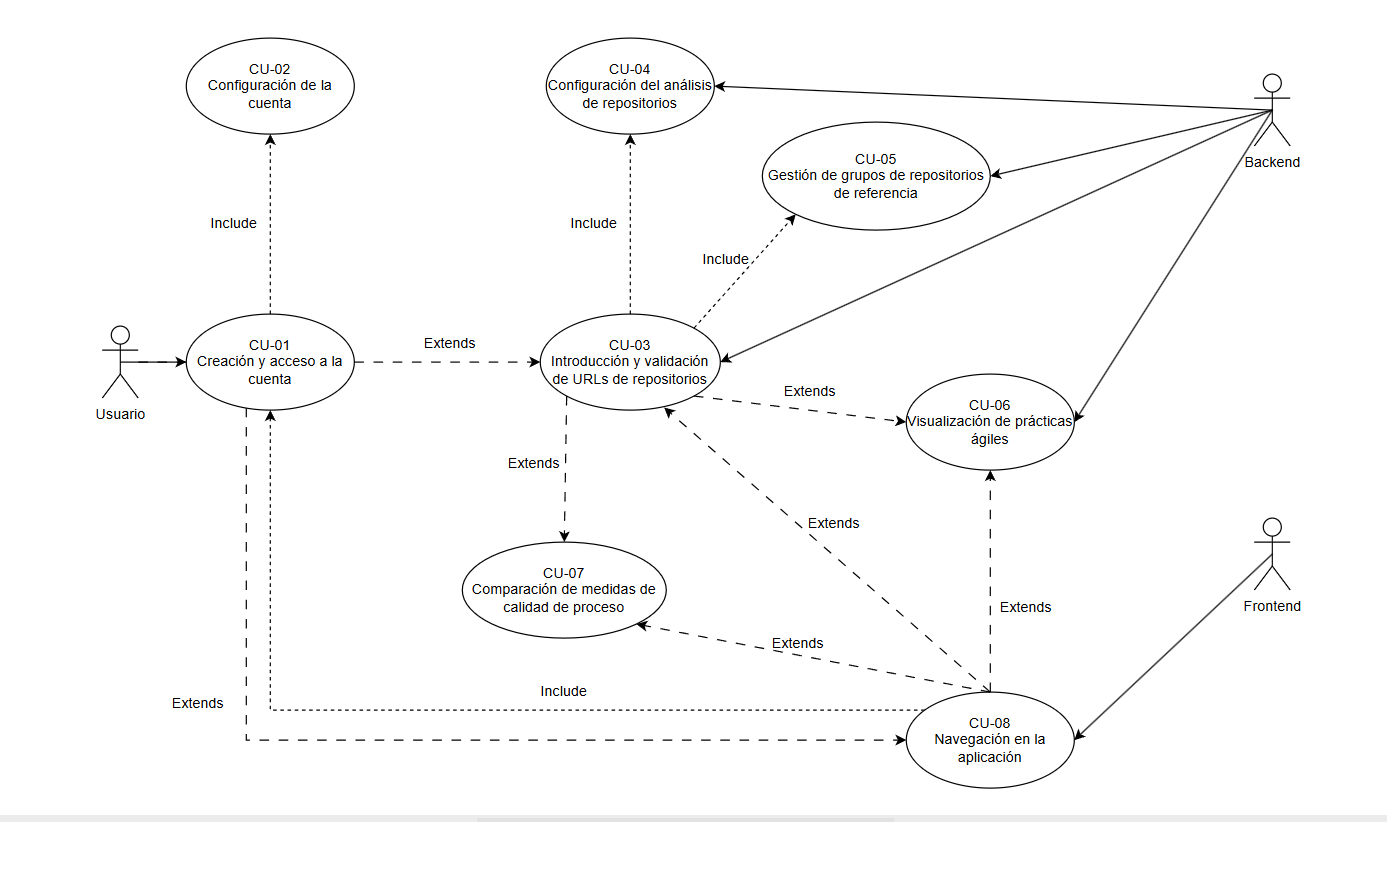
\includegraphics[width=0.8\textwidth]{img/Diagrama-casos-de-uso.png}
\caption{Diagrama de casos de uso general}
\label{fig:Diagrama-casos-de-uso}
\end{figure}

% Caso de Uso 1 -> Creación y acceso a la cuenta
\clearpage
\begin{table}[p]
	\centering
	\begin{tabularx}{\linewidth}{ p{0.21\columnwidth} p{0.71\columnwidth} }
        \toprule
        \textbf{CU-1}    & \textbf{Creación y acceso a la cuenta} \\
        \toprule
        \textbf{Versión}              & 1.0 \\
        \textbf{Autor}                & Lucas Olmedo Diéz \\
        \textbf{Requisitos asociados} & RF-01, RF-02 \\
        \textbf{Descripción}          & Permite al usuario crear una cuenta y acceder a la aplicación mediante inicio de sesión. \\
        \textbf{Precondición}         & El usuario debe introducir un usuario único y una contraseña válida \\
        \textbf{Acciones}             &
        \begin{enumerate}
            \def\labelenumi{\arabic{enumi}.}
            \tightlist
            \item El usuario accede a la página de registro o inicio de sesión.
            \item El usuario introduce los datos necesarios (usuario y contraseña).
            \item El sistema verifica la validez de los datos.
            \item El sistema registra al usuario o permite el acceso según corresponda.
        \end{enumerate}\\
        \textbf{Postcondición}        & El usuario ha creado una cuenta o ha accedido a su perfil. \\
        \textbf{Excepciones}          & Datos incorrectos o cuenta inexistente/ya registrada. \\
        \textbf{Importancia}          & Alta \\
        \bottomrule
    \end{tabularx}
    \caption{CU-1 Creación y acceso a la cuenta.}
\end{table}

% Caso de Uso 2 -> Configuración de la cuenta
\clearpage
\begin{table}[p]
    \centering
    \begin{tabularx}{\linewidth}{ p{0.21\columnwidth} p{0.71\columnwidth} }
        \toprule
        \textbf{CU-2}    & Configuración de la cuenta \\
        \midrule
        \textbf{Versión}              & 1.0 \\
        \textbf{Autor}                & Lucas Olmedo Diéz \\
        \textbf{Requisitos asociados} & RF-02, RF-03 \\\
        \textbf{Descripción}          & Permite al usuario cambiar la contraseña y modificar el idioma de la aplicación. \\
        \textbf{Precondición}         & El usuario debe haber iniciado sesión. \\
        \textbf{Acciones}             &
        \begin{enumerate}
            \def\labelenumi{\arabic{enumi}.}
            \tightlist
            \item El usuario accede a la sección de configuración.
            \item Selecciona cambiar contraseña o idioma.
            \item El sistema valida y aplica los cambios.
        \end{enumerate}\\
        \textbf{Postcondición}        & Se actualizan las preferencias del usuario. \\
        \textbf{Excepciones}          & \\
        \textbf{Importancia}          & Media \\
        \bottomrule
    \end{tabularx}
    \caption{CU-2 Configuración de la cuenta.}
\end{table}

% Caso de Uso 3 -> Introducción y validación de URLs
\clearpage
\begin{table}[p]
    \centering
    \begin{tabularx}{\linewidth}{ p{0.21\columnwidth} p{0.71\columnwidth} }
        \toprule
        \textbf{CU-3}    & Introducción y validación de URLs de repositorios \\
        \midrule
        \textbf{Versión}              & 1.0 \\
        \textbf{Autor}                & Lucas Olmedo Diéz \\
        \textbf{Requisitos asociados} & RF-04 \\
        \textbf{Descripción}          & Permite al usuario introducir URLs de repositorios GitHub y valida su formato y accesibilidad. \\
        \textbf{Precondición}         & El usuario ha iniciado sesión. \\
        \textbf{Acciones}             &
        \begin{enumerate}
            \def\labelenumi{\arabic{enumi}.}
            \tightlist
            \item El usuario introduce una o varias URLs.
            \item El sistema valida la estructura y el acceso.
            \item Se informa al usuario del resultado.
        \end{enumerate}\\
        \textbf{Postcondición}        & Se aceptan o rechazan las URLs introducidas. \\
        \textbf{Excepciones}          & URL malformada o repositorio no accesible. \\
        \textbf{Importancia}          & Alta \\
        \bottomrule
    \end{tabularx}
    \caption{CU-3 Introducción y validación de URLs de repositorios.}
\end{table}

% CU-4: Configuración del análisis de repositorios
\clearpage
\begin{table}[p]
    \centering
    \begin{tabularx}{\linewidth}{ p{0.21\columnwidth} p{0.71\columnwidth} }
        \toprule
        \textbf{CU-4} & Configuración del análisis de repositorios \\
        \midrule
        \textbf{Versión} & 1.0 \\
        \textbf{Autor} & Lucas Olmedo Díez \\
        \textbf{Requisitos asociados} & RF-05, RF-06, RF-07,\ RF-08 \\
        \textbf{Descripción} & Permite al usuario configurar cómo se analizarán los datos del repositorio: intervalos absolutos o relativos, número de días para calcular las métricas temporales, períodos de los intervalos. \\
        \textbf{Precondición} & El usuario debe haber elegido la opción de "Analizar por intervalos de tiempo". \\
        \textbf{Acciones} &
        \begin{enumerate}
            \def\labelenumi{\arabic{enumi}.}
            \tightlist
            \item El usuario selecciona si desea usar fechas absolutas o relativas.
            \item Ajusta manualmente los intervalos de fechas específicos.
            \item Elige el tipo de intervalos para segmentar la información.
            \item (Opcional) Se cambia el númerod e días usado para obtener métricas de calidad temporales.
        \end{enumerate}\\
        \textbf{Postcondición} & El sistema ha almacenado la configuración de análisis para ser utilizada en el cálculo de métricas. \\
        \textbf{Excepciones} & Intervalos inválidos, número de días no válido, configuración incompleta. \\
        \textbf{Importancia} & Alta \\
        \bottomrule
    \end{tabularx}
    \caption{CU-4 Configurar análisis del repositorio}
\end{table}

% CU-5: Gestión de grupos de repositorios de referencia
\clearpage
\begin{table}[p]
    \centering
    \begin{tabularx}{\linewidth}{ p{0.21\columnwidth} p{0.71\columnwidth} }
        \toprule
        \textbf{CU-5} & Gestión de grupos de repositorios de referencia \\
        \midrule
        \textbf{Versión} & 1.0 \\
        \textbf{Autor} & Lucas Olmedo Díez \\
        \textbf{Requisitos asociados} & RF-09, RF-10 \\
        \textbf{Descripción} & Permite al usuario cargar o borrar grupos de repositorios previamente guardados para usarlos como referencia comparativa en los análisis. \\
        \textbf{Precondición} & El usuario debe haber hecho algún análisis previo con el que se guardaron repositorios de referencia. \\
        \textbf{Acciones} &
        \begin{enumerate}
            \def\labelenumi{\arabic{enumi}.}
            \tightlist
            \item El usuario accede a la sección de gestión de repositorios guardados.
            \item Selecciona un grupo de repositorios guardado previamente y lo carga.
            \item (Opcional) Elimina uno o más grupos guardados si lo desea.
        \end{enumerate}\\
        \textbf{Postcondición} & Los grupos seleccionados han sido cargados o eliminados exitosamente. \\
        \textbf{Excepciones} & No hay grupos guardados disponibles o error en la carga/borrado. \\
        \textbf{Importancia} & Media \\
        \bottomrule
    \end{tabularx}
    \caption{CU-5 Gestionar grupos de repositorios de comparación}
\end{table}

% CU-6: Visualización de prácticas ágiles
\clearpage
\begin{table}[p]
    \centering
    \begin{tabularx}{\linewidth}{ p{0.21\columnwidth} p{0.71\columnwidth} }
        \toprule
        \textbf{CU-6} & Visualización de prácticas ágiles \\
        \midrule
        \textbf{Versión} & 1.0 \\
        \textbf{Autor} & Lucas Olmedo Díez \\
        \textbf{Requisitos asociados} & RF-11 \\
        \textbf{Descripción} & Permite al usuario visualizar el grado de adopción de buenas prácticas ágiles evaluadas automáticamente por el sistema a partir de los datos del repositorio. \\
        \textbf{Precondición} & Se han introducido URLS válidad y parámetros del análisis correctos. \\
        \textbf{Acciones} &
        \begin{enumerate}
            \def\labelenumi{\arabic{enumi}.}
            \tightlist
            \item El sistema muestra los resultados del análisis de buenas prácticas en formato gráfico y textual.
            \item El usuario puede consultar qué reglas se cumplen, cuáles no, y por qué.
        \end{enumerate}\\
        \textbf{Postcondición} & El usuario ha accedido a la información evaluada y entendible de las prácticas ágiles del repositorio. \\
        \textbf{Excepciones} & No se han podido calcular algunas reglas por errores en añgún repositorio. \\
        \textbf{Importancia} & Alta \\
        \bottomrule
    \end{tabularx}
    \caption{CU-6 Visualizar evaluación de buenas prácticas ágiles}
\end{table}

% CU-7: Comparación de medidas de calidad de proceso
\clearpage
\begin{table}[p]
    \centering
    \begin{tabularx}{\linewidth}{ p{0.21\columnwidth} p{0.71\columnwidth} }
        \toprule
        \textbf{CU-7} & Comparación de medidas de calidad de proceso \\
        \midrule
        \textbf{Versión} & 1.0 \\
        \textbf{Autor} & Lucas Olmedo Díez \\
        \textbf{Requisitos asociados} & RF-12 \\
        \textbf{Descripción} & Permite comparar visualmente las métricas del repositorio analizado con las de los repositorios de referencia cargados. \\
        \textbf{Precondición} & El repositorio analizado y al menos un grupo de referencia, junto a sus medidas de calidad deben estar cargados. \\
        \textbf{Acciones} &
        \begin{enumerate}
            \def\labelenumi{\arabic{enumi}.}
            \tightlist
            \item El usuario accede a la sección de comparación.
            \item El sistema genera y muestra listas comparativas de las métricas seleccionadas.
            \item El usuario interpreta la comparación en función de los valores visualizados.
        \end{enumerate}\\
        \textbf{Postcondición} & El usuario obtiene una visión comparativa clara del estado de su proyecto. \\
        \textbf{Excepciones} & Error al cargar los datos de referencia o métricas incomparables. \\
        \textbf{Importancia} & Alta \\
        \bottomrule
    \end{tabularx}
    \caption{CU-7 Comparar con repositorios de referencia}
\end{table}

% CU-8: Navegar por la aplicación
\clearpage
\begin{table}[p]
    \centering
    \begin{tabularx}{\linewidth}{ p{0.21\columnwidth} p{0.71\columnwidth} }
        \toprule
        \textbf{CU-8} & Navegar por la aplicación \\
        \midrule
        \textbf{Versión} & 1.0 \\
        \textbf{Autor} & Lucas Olmedo Díez \\
        \textbf{Requisitos asociados} & RF-11, RF-03 \\
        \textbf{Descripción} & Permite al usuario desplazarse cómodamente por las diferentes secciones de la aplicación (login, análisis, comparación, configuración, etc.), garantizando una experiencia de usuario fluida. \\
        \textbf{Precondición} & El usuario debe haber iniciado sesión. La aplicación debe estar desplegada correctamente. \\
        \textbf{Acciones} &
        \begin{enumerate}
            \def\labelenumi{\arabic{enumi}.}
            \tightlist
            \item El usuario interactúa con los tabs y botones de navegación disponibles.
            \item El sistema muestra el contenido correspondiente sin errores.
        \end{enumerate}\\
        \textbf{Postcondición} & El usuario ha accedido correctamente a las diferentes funcionalidades sin fricciones. \\
        \textbf{Excepciones} & Error de carga, o comportamiento inesperado. \\
        \textbf{Importancia} & Alta \\
        \bottomrule
    \end{tabularx}
    \caption{CU-8 Navegar por la aplicación}
\end{table}
\apendice{Especificación de diseño}

\section{Introducción}
En este apartado del anexo se van a documentar todos los aspectos relacionados al diseño del proyecto, y como consecuencia, de la aplicación desarrollada en el mismo. Se describirán los componentes y entidades que forman el proyecto, y cómo estos se relacionan entre sí, con el objetivo de detallar cómo logran implementar los objetivos del proyecto ya mencionados.

La manera principal de explicar los componentes, datos y entidades del diseño del proyecto será la de varios diagramas que ayuden a comprender el funcionamiento y relaciones que existen entre los mismos, incluyendo sus atributos y características.

\section{Diseño de datos}

En esta sección se describirá el diseño de los datos del sistema. Para ello se detallará una serie de diagramas entidad-relación que detallarán cómo se relacionan estos entre sí, mostrando los atributos más influyentes de cada uno. 

\begin{figure}[H]
\centering
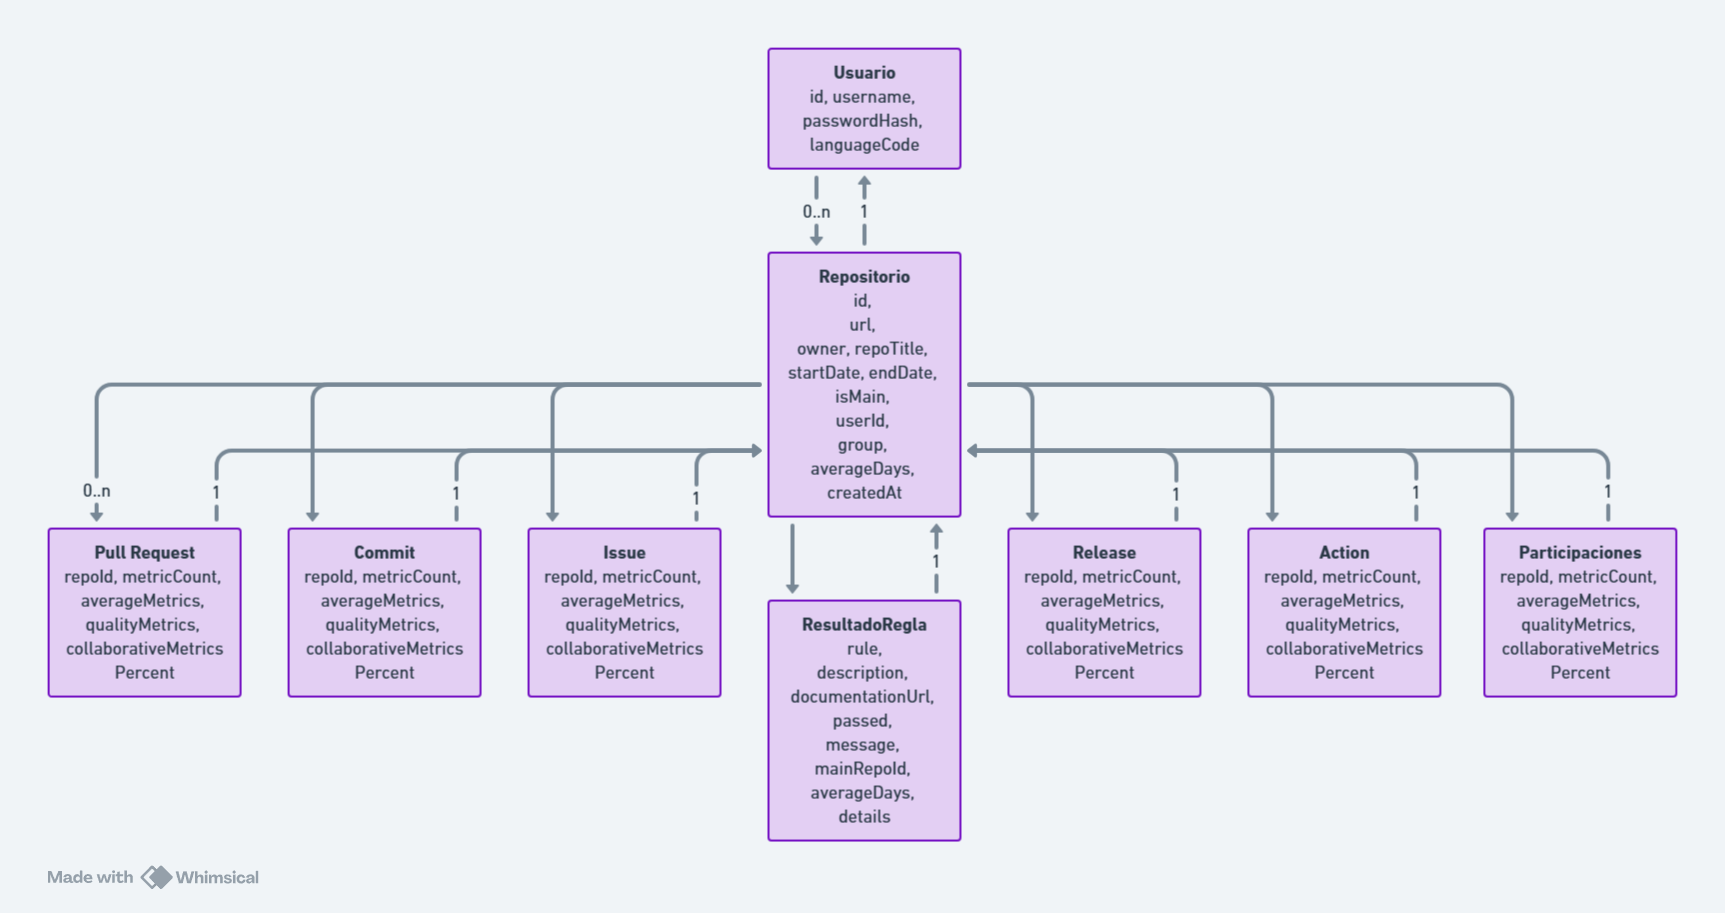
\includegraphics[width=0.8\textwidth]{img/Diagrama-entidad-relacion.png}
\caption{Diagrama Entidad - Relación de la aplicación del proyecto}
\label{fig:DiagramaER}
\end{figure}

\begin{figure}[H]
\centering
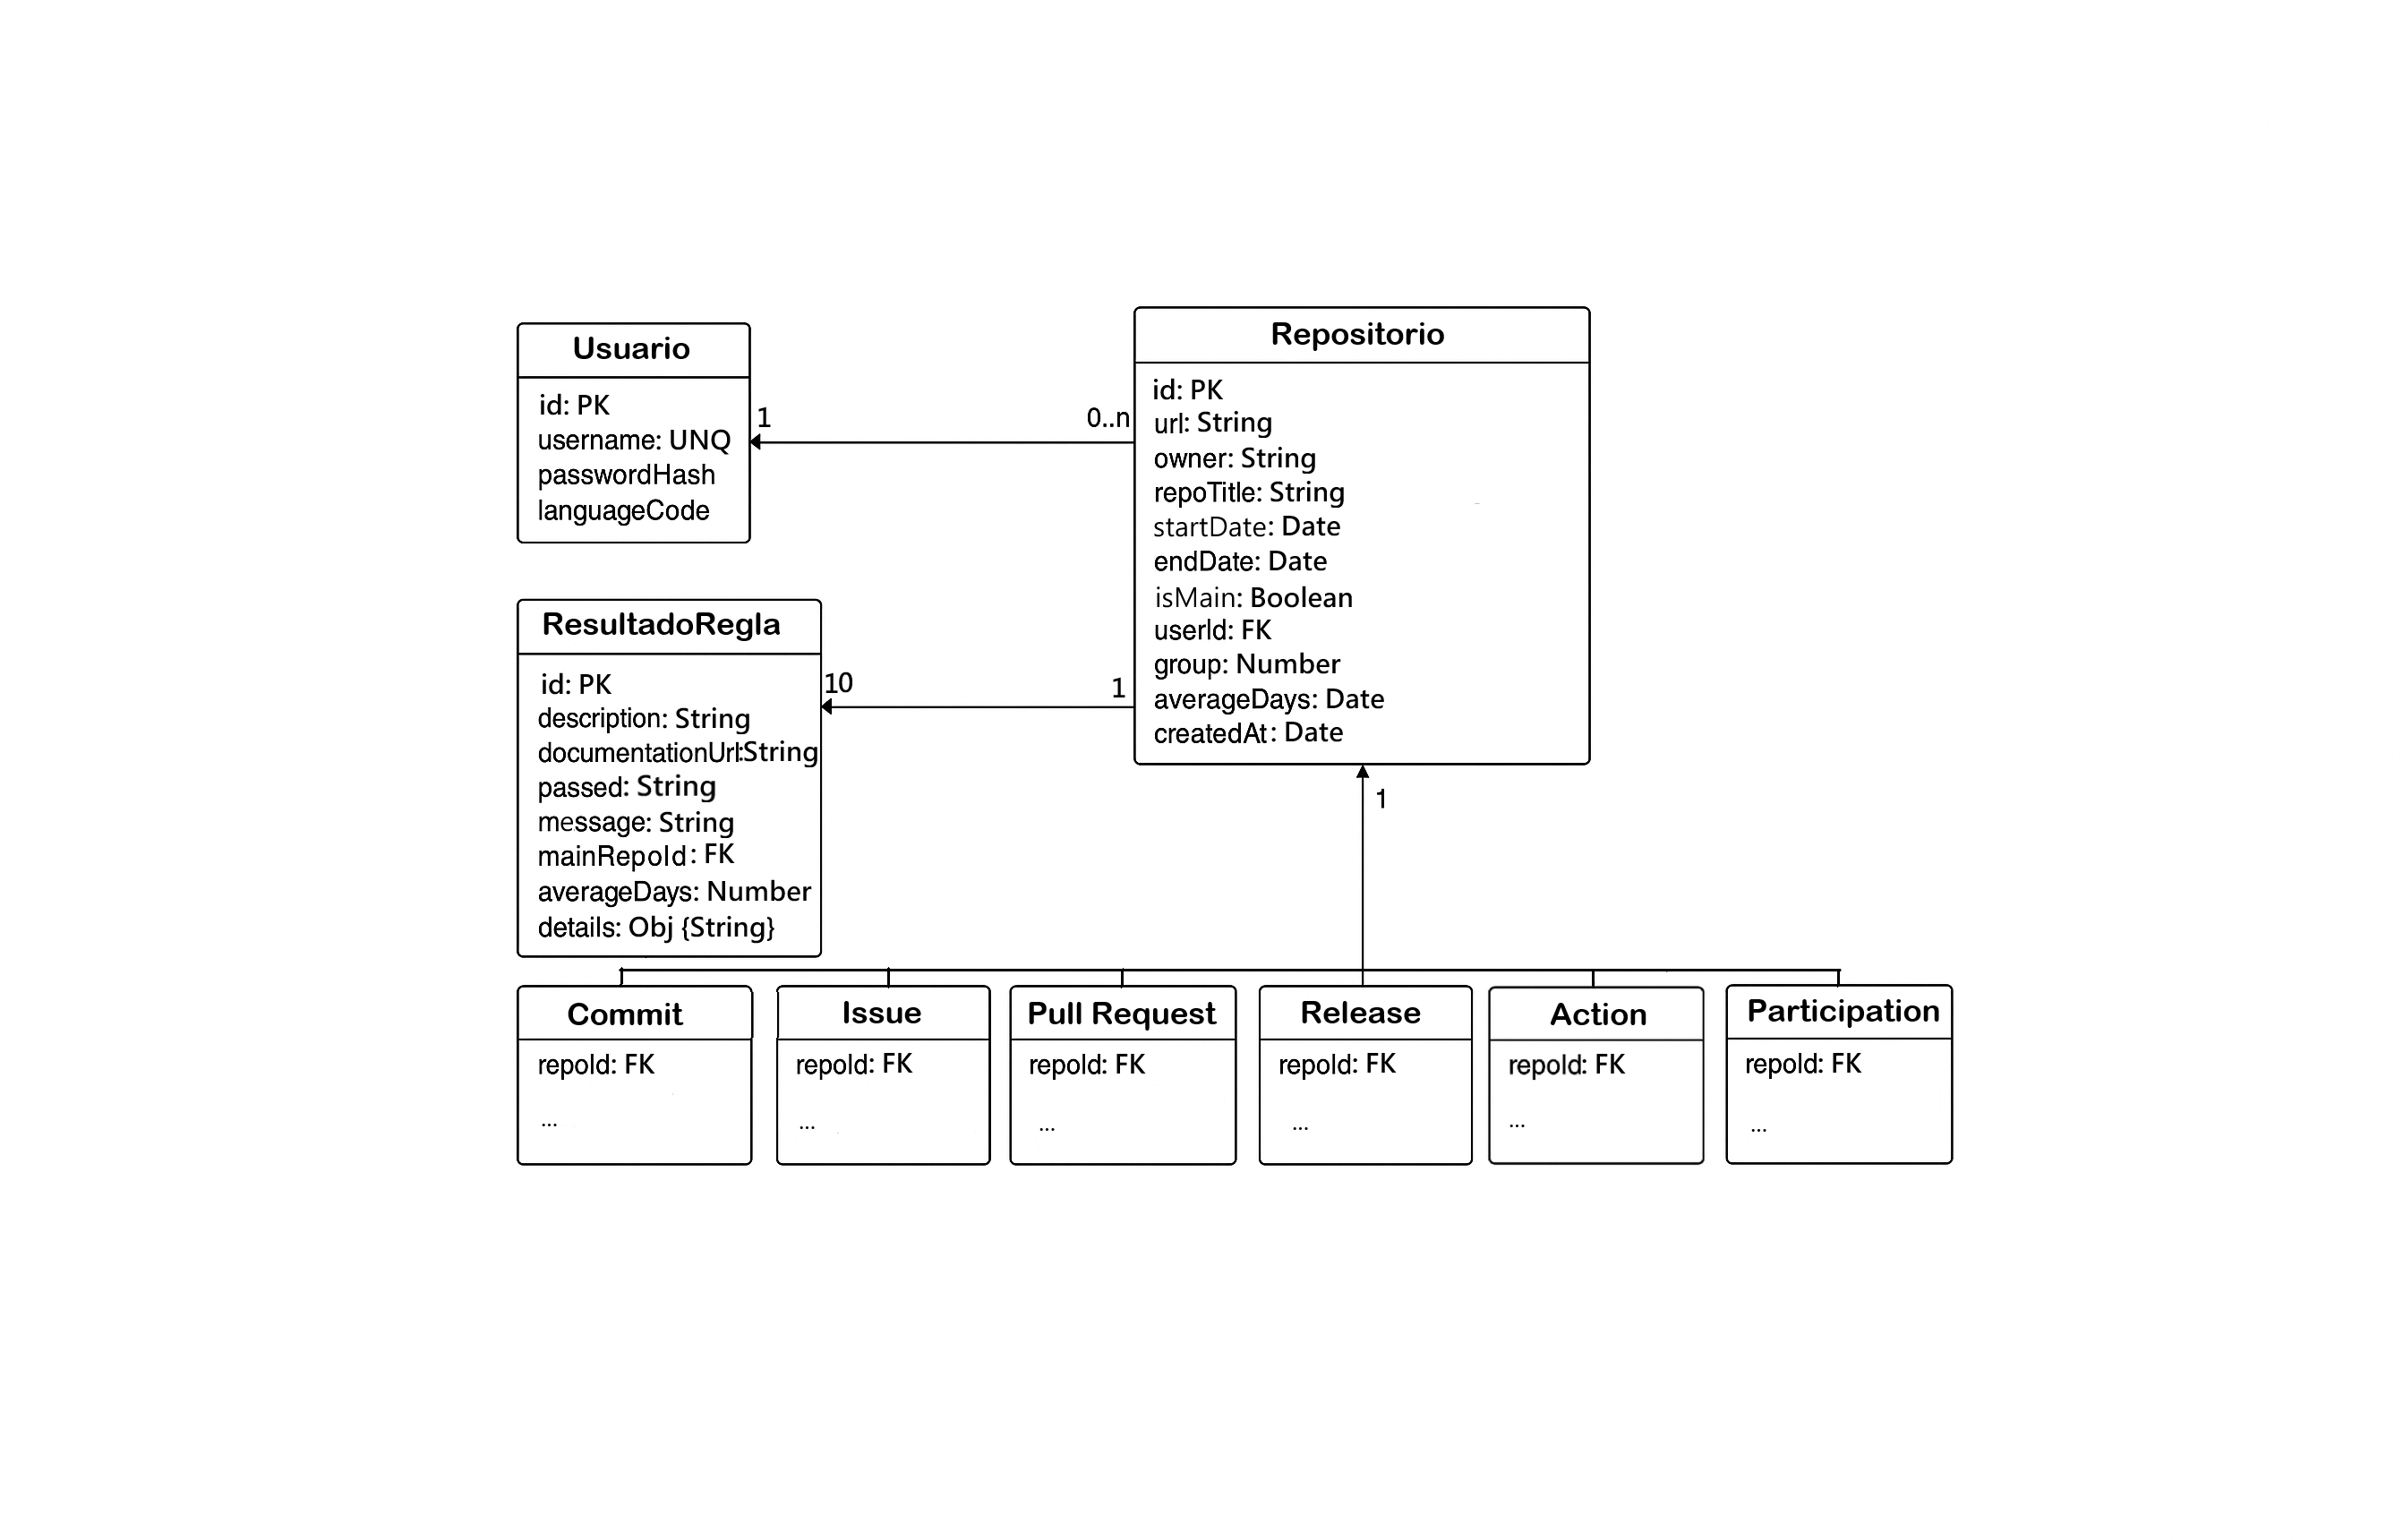
\includegraphics[width=0.8\textwidth]{img/Diagrama-entidad-relacionUML.png}
\caption{Diagrama Entidad - Relación UML de la aplicación del proyecto}
\label{fig:DiagramaER_UML}
\end{figure}

\subsection{Entidades del Sistema}
\begin{itemize}
	\item \textbf{Usuario}: Representa a los usuarios de la aplicación.
		\begin{itemize}
			\item \textbf{id}: Identificador único del usuario.
			\item \textbf{username}: Nombre de usuario, único en el sistema.
			\item \textbf{passwordHash}: Contraseña encriptada.
			\item \textbf{languageCode}: Código del idioma que utiliza el usuario.
		\end{itemize}

	\item \textbf{Repositorio}: Contiene los datos de un repositorio analizado.
		\begin{itemize}
			\item \textbf{id}: Identificador único del repositorio analizado.
			\item \textbf{url}: Dirección URL del repositorio.
			\item \textbf{owner}: Nombre del propietario del repositorio.
			\item \textbf{repoTitle}: Título o nombre del repositorio.
			\item \textbf{startDate}: Fecha de inicio del análisis.
			\item \textbf{endDate}: Fecha de finalización del análisis.
			\item \textbf{isMain}: Indica si es el repositorio principal o de referencia.
			\item \textbf{userId}: Identificador del usuario propietario del repositorio.
			\item \textbf{group}: Número de grupo comparativo de referencia (si aplica).
			\item \textbf{averageDays}: Número de días promedio utilizado en métricas de media.
			\item \textbf{createdAt}: Fecha de creación del análisis.
		\end{itemize}

	\item \textbf{ResultadoRegla}: Almacena el resultado del análisis de buenas prácticas.
		\begin{itemize}
			\item \textbf{rule}: Nombre de la regla evaluada.
			\item \textbf{description}: Descripción de la regla.
			\item \textbf{documentationUrl}: Enlace a la documentación de la regla.
			\item \textbf{passed}: Indica si la regla fue superada.
			\item \textbf{message}: Comentario asociado al resultado.
			\item \textbf{mainRepoId}: Repositorio principal evaluado.
			\item \textbf{averageDays}: Días promedio utilizados en la evaluación.
            \item \textbf{details}: Medidas que evalúa la regla y su evaluación
		\end{itemize}

	\item \textbf{Métricas (\textit{Commit}, \textit{Issue}, \textit{Pull Request}, \textit{Release}, \textit{Action}, \textit{Participaciones}}: Cada una de estas entidades representa métricas agregadas de su tipo específico, siempre vinculadas a un único repositorio mediante la clave \textbf{repoId}.
		\begin{itemize}
			\item \textbf{repoId}: Repositorio al que pertenece la métrica.
			\item \textbf{metricCount}: Total numérico de la métrica (Por ejemplo \textit{commitCount}).
			\item \textbf{averageMetrics}: Promedio de aparición o cierre de la métrica (Por ejemplo averageClosedIssues).
			\item \textbf{qualityMetrics}: Atributos que reflejan medidas de calidad de proceso que dependen del tipo de métrica (Por ejemplo el porcentaje de issues con imágenes, o el número de ficheros workflow ejecutados con éxito).
			\item \textbf{collaborativeMetricsPercent}: Porcentaje de instancias de la métrica realizadas de forma colaborativa.
		\end{itemize}
    \end{itemize}

\subsection{Relaciones entre Entidades}
\begin{itemize}
	\item \textbf{Usuario - Repositorio}:
	\begin{itemize}
		\item Un \textbf{Usuario} posee \textbf{0..n} instancias de \textbf{Repositorio}.
		\item Un \textbf{Repositorio} pertenece a exactamente un \textbf{Usuario}.
	\end{itemize}

    \item \textbf{Repositorio - ResultadoRegla}:
	\begin{itemize}
		\item Un \textbf{Repositorio (principal)} genera \textbf{10} resultados de \textbf{ResultadoRegla} (Uno por cada una de las 10 reglas definidas).
		\item Un \textbf{ResultadoRegla} se asocia a exactamente un \textbf{Repositorio (principal)}.
	\end{itemize}

	\item \textbf{Repositorio - Métrica}:
	\begin{itemize}
		\item Un \textbf{Repositorio} tiene exactamente una instancia de métricas para cada uno de los siguientes: \textbf{\textit{Commit}}, \textbf{\textit{Issue}}, \textbf{\textit{Pull Request}}, \textbf{\textit{Release}}, \textbf{\textit{Action}}, \textbf{Participaciones}.
		\item Cada una de estas métricas pertenece a un solo \textbf{Repositorio}.
	\end{itemize}
\end{itemize}

\section{Diseño arquitectónico}

El diseño de la arquitectura de la aplicación se divide en 2 partes fundamentales: un frontend de Angular dividido en componentes y servicios, y un backend de Node js que usa controladores para ejecutar funciones y modelos para la base de datos. La separación del frontEnd y el backend garantiza la separación de responsabilidades, lo que se ve reforzado por los componentes del frontend y los controladores del backend, que separan aún más las reponsabilidades internamente. Los componentes y controladores siguen el principio \textit{Open-Closed} de programación, permitiendo añadir nuevas funcionalidades sin necesidad de alterar el resto del código (Por ejemplo añadir nuevas pantallas o reglas).

Esta arquitectura y sus divisones en directorios se muestran de una forma más detallada y visual en la siguiente figura:

\begin{figure}[H]
\centering
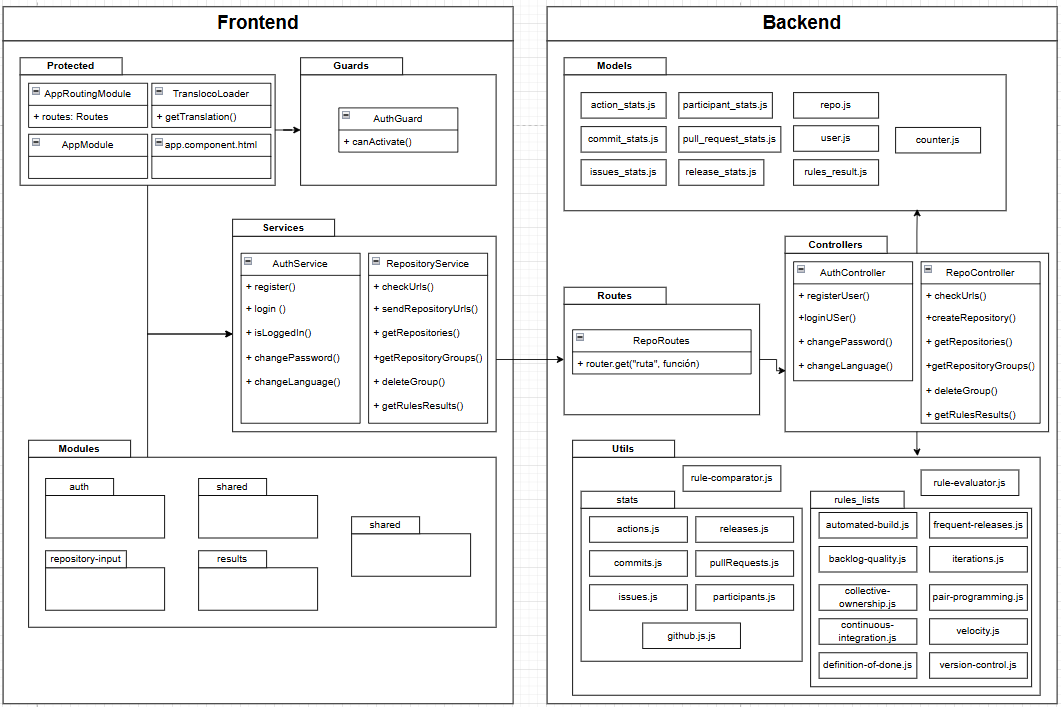
\includegraphics[width=0.8\textwidth]{img/Diagrama-paquetes.png}
\caption{Diagrama del diseño arquitectónico}
\label{fig:DiagramaDirectorios}
\end{figure}

A continuación se detallará en mayor medida las funcionalidades de cada parte tanto del backend como el frontend

\begin{itemize}
    \item \textbf{Frontend}:
    \begin{itemize}
    	\item \textbf{Guards}: Incluye el fichero auth-guard.guard.ts, que se encarga de reforzar la seguridad de acceso a la aplicación bloqueando accesos a las distintas URLs sin haber iniciado sesión
    	\item \textbf{Modules}: Contiene casi toda la lógica del fontend, incluyendo todos los componentes .ts, .html y .css de cada parte de la página web, encargándose estos de definir la lógica, estructura de la página y estilos de maquetación de la misma, respectivamente. Se puede apreciar una mejor representación de su estructura en la figura siguiente. Se compone de las siguientes carpetas:
            \begin{itemize}
                \item \textbf{auth}: Da forma a la pantalla de inicio y usa sus componentes hijos para cambiar entre formulario de registro, inicio de sesión o cambio de contraseña.
                \item \textbf{repository-input}: Se encarga de la pantalla donde el usuario introduce los repositorios y configura el análisis.
                \item \textbf{results}: Muestra la pantalla de los resultados de las prácticas ágiles.
                \item \textbf{statistics}: Muestra la pantalla de comparación de métricas de proceso, que se compone de 2 listas comparativas entre repositorios.
                \item \textbf{shared}: Contiene componentes que usan varias pantallas, como lo son el \textit{header} y el \textit{footer}.
            \end{itemize}
    	\item \textbf{Protected}: Incluye los módulos y componentes más importantes del código, como las definiciones de las rutas, las librerías y componentes a usar, el fichero html principal y el cargador de la librería de traducciones "Transloco".
    	\item \textbf{Services}: Incluye los ficheros auth.service.ts y repository.service.ts, que utilizarán peticiones HttpClient para llamar a las funciones correspondientes de los controladores del backend y utilizar sus funciones.
    \end{itemize}

    \begin{figure}[H]
    \centering
    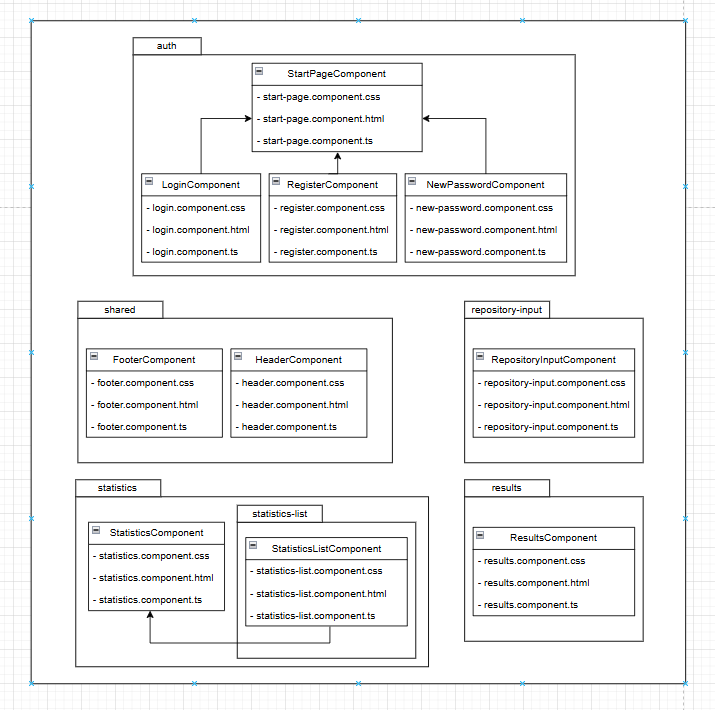
\includegraphics[width=0.8\textwidth]{img/Diagrama-detalle-modules.png}
    \caption{Diagrama del directorio \textbf{modules} del frontend}
    \label{fig:DiagramaDetalleModules}
    \end{figure}
    
    \item \textbf{Backend}:
    \begin{itemize}
    	\item \textbf{controllers}: Se compone de authController.js y repoController.js, que son los ficheros con las funciones principales que definen la lógica general del código relacionado con la autentificación de usuarios y el manejo de repositorios, respectivamente. Para ello utilizarán los modelos definidos en "Models" y las funciones menores definidad en "utils"
        \item \textbf{routes}: Su fichero repoRoutes.js define las rutas que usarán los servicios del frontend para acceder a las funciones de los controllers.
    	\item \textbf{models}: Contiene los ficheros que definen cada tabla de la base de datos a través de la librería mongoose.
    	\item \textbf{utils}: Contiene las funciones secundarias necesarias que usará repoController.js. Hay un fichero y función pequeña para cada tabla de métricas (\textit{commits}, \textit{issues}, etc), junto a un fichero github.js que obtiene datos del repositorio importantes como el título y autor; y para cada práctica ágil definida (Version control, Iterations, etc), además de algunas funciones de ayuda comorule-comparator.js, que compara las medidas de calidad de proceso entre el repositorio principal y los repositorios de referencia para evaluar las reglas
    \end{itemize}
\end{itemize}

La particularidad de haber dividido el código entre frontend y backend refuerza enormemente la flexibilidad y la escalabilidad del diseño, así como la legibilidad y mantenimiento del código.

\subsection{Patrones de diseño}

No toda la flexibilidad, escalabilidad y robustez se deben sólo a la estructura interna del código, sino también a los patrones de diseño \cite{gamma1994design} aplicados. Estos patrones mejoran de la calidad del código y la reutilización de componentes, y refuerzan la legibilidad y mantenibilidad, así como una comunicación más clara entre desarrolladores o, en el caso del desarrollo de este proyecto, la comunicación entre el alumno autor y el tutor del TFG. 

Para el diseño de este proyecto se han tenido en cuenta los principios SOLID \cite{solid_principles} que, junto a ciertos patrones de diseño concretos, han sido de especial utilidad en una arquitectura como lo es la ya descrita de este proyecto. A continuación se detallan los patrones y principios de diseño más relevantes considerados:

\begin{itemize}
    \item \textbf{Patrón fachada}: Este patrón se aplica especialmente en la comunicación entre el frontend y el backend a través de los servicios (AuthService, RepositoryService). Estos actúan como una "fachada" que simplifica el acceso a múltiples funciones complejas del backend.
    \begin{itemize}
        \item \textbf Facilita la interacción del frontend con el backend al ocultar la complejidad de las peticiones HTTP y lógica interna.
        \item \textbf Mejora la cohesión y disminuye el acoplamiento entre componentes.
        \item \textbf Permite modificar el backend sin afectar al frontend, siempre que la fachada (servicio) mantenga su interfaz.
        \item \textbf Aumenta la reutilización y testeo de código, al centralizar la lógica de acceso a datos.
    \end{itemize}
    
    \item \textbf{Principio Abierto / Cerrado}: Este principio se observa en los controladores y módulos, los cuales están diseñados para permitir extensiones (nuevas rutas, pantallas, reglas) sin necesidad de modificar el código ya existente.
    \begin{itemize}
        \item \textbf{Beneficio}: Facilita la adición de nuevas funcionalidades de forma segura.
        \item \textbf{Beneficio}: Reduce el riesgo de introducir errores al mantener el código existente intacto.
        \item \textbf{Beneficio}: Mejora la mantenibilidad y escalabilidad del sistema.
        \item \textbf{Beneficio}: Favorece el desarrollo ágil, permitiendo iteraciones rápidas.
    \end{itemize}
    
    \item \textbf{Patrón Inyección de Dependencias}:  Angular, por diseño, utiliza inyección de dependencias para los servicios (AuthService, RepositoryService, HttpClient, etc.), permitiendo declarar dependencias en los constructores.
    \begin{itemize}
        \item \textbf{Beneficio}: Aumenta la modularidad del código y promueve el bajo acoplamiento.
        \item \textbf{Beneficio}: Mejora la reutilización y mantenimiento del código.
        \item \textbf{Beneficio}: Permite una mayor flexibilidad en la configuración de servicios.
    \end{itemize}
    
    \item \textbf{Principio de Separación de responsabilidades}: Toda la arquitectura se basa en una clara división de responsabilidades: frontend vs backend, componentes vs servicios, controladores vs modelos, etc.
    \begin{itemize}
        \item \textbf{Beneficio}: Mejora la legibilidad del código al estar organizado por función.
        \item \textbf{Beneficio}: Permite a varios desarrolladores trabajar en paralelo en diferentes áreas del sistema.
        \item \textbf{Beneficio}: Reduce errores al evitar dependencias innecesarias entre módulos.
        \item \textbf{Beneficio}: Favorece la reutilización de módulos y componentes en otros proyectos.
    \end{itemize}
    
    \item \textbf{Patrón Controlador}: Utilizado en el backend para organizar la lógica relacionada con diferentes dominios (AuthController, RepoController). Cada controlador es responsable de orquestar las funciones relacionadas con una entidad del sistema.
    \begin{itemize}
        \item \textbf{Beneficio}: Centraliza la lógica de cada parte del sistema, facilitando su entendimiento y modificación.
        \item \textbf{Beneficio}: Permite escalar el sistema con facilidad al añadir nuevos controladores según se necesiten.
        \item \textbf{Beneficio}: Mejora la trazabilidad de errores
        \item \textbf{Beneficio}: Favorece el desacoplamiento entre la lógica de negocio y la lógica de acceso a datos.
    \end{itemize}
    
    \item \textbf{Patrón decorador}: En Angular se emplea el patrón decorador mediante anotaciones como @Component, @Injectable, @Input, @Output, que permiten añadir información a las clases, propiedades o métodos sin modificar directamente su implementación.
    \begin{itemize}
        \item \textbf{Beneficio}: Permite extender funcionalidades de manera flexible sin modificar el código original.
        \item \textbf{Beneficio}: Aumenta la legibilidad y organización del código, permitiendo declarar claramente el propósito de cada clase o propiedad.
        \item \textbf{Beneficio}: Mejora la reutilización de componentes a través de la configuración por propiedades decoradas (@Input(), usado en \textbf{StatisticsListComponent}).
    \end{itemize}
\end{itemize}

\section{Diseño procedimental}
En esta sección se describirá el flujo a seguir en las tareas más relevantes que se hacen en la aplicación mediante los \textbf{Casos de Uso (CU)} definidos previamente

\subsection*{CU1 - Creación y acceso a la cuenta}

Este caso de uso permite al usuario crear una cuenta en la aplicación o acceder mediante inicio de sesión. Está dirigido a nuevos usuarios o a aquellos que desean autenticarse. El sistema valida la información antes de registrar o permitir el acceso como se puede ver en la figura~\ref{fig:DiagramaCU1})

\textbf{Pasos que sigue el CU:}
\begin{enumerate}
  \item El usuario accede a la página de registro o inicio de sesión.
  \item Introduce su usuario y contraseña.
  \item El sistema verifica los datos ingresados.
  \item Según el caso, se crea una nueva cuenta o se otorga acceso.
\end{enumerate}

\begin{figure}[H]
\centering
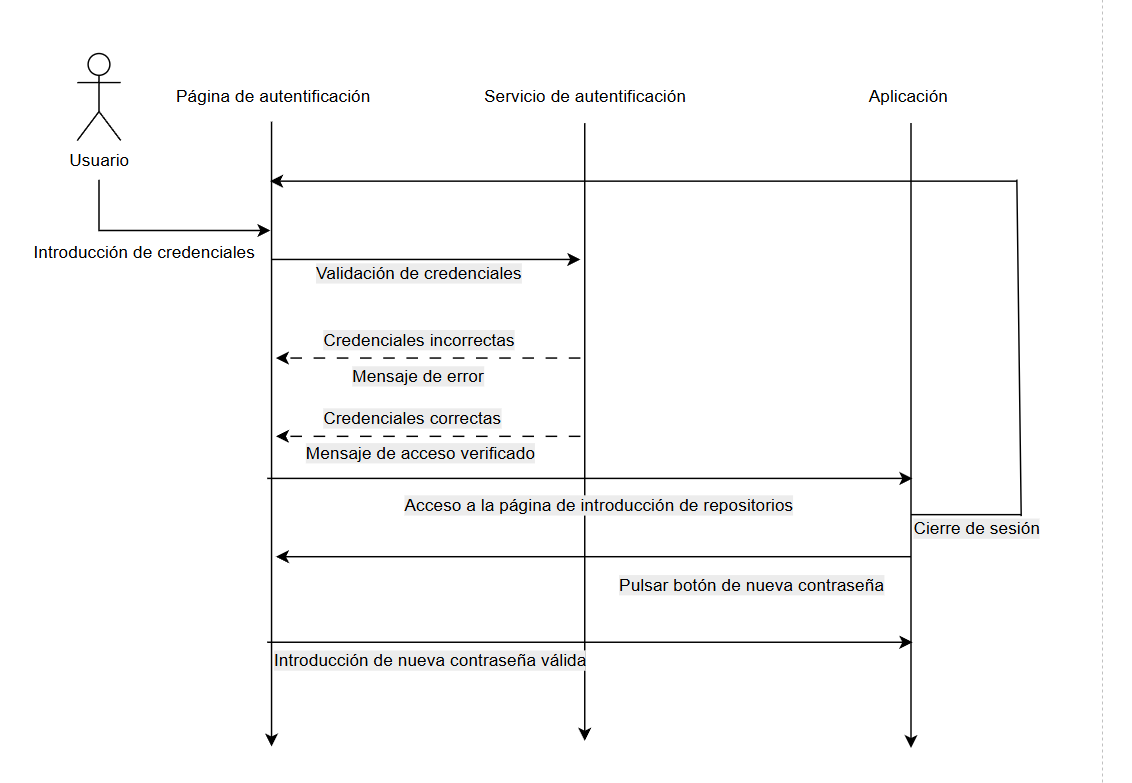
\includegraphics[width=0.8\textwidth]{img/DiagramaCU1.png}
\caption{Diagrama del caso de uso CU1}
\label{fig:DiagramaCU1}
\end{figure}

\subsection*{CU2 - Configuración de la cuenta}

Permite al usuario modificar su configuración de cuenta, como el idioma o la contraseña. Es necesario haber iniciado sesión previamente. El sistema valida y aplica los cambios, tal como se muestra en la figura~\ref{fig:DiagramaCU2}.

\textbf{Pasos que sigue el CU:}
\begin{enumerate}
  \item El usuario accede a la sección de configuración.
  \item Selecciona si desea cambiar la contraseña o el idioma.
  \item El sistema valida los datos ingresados y aplica los cambios.
\end{enumerate}

\begin{figure}[H]
\centering
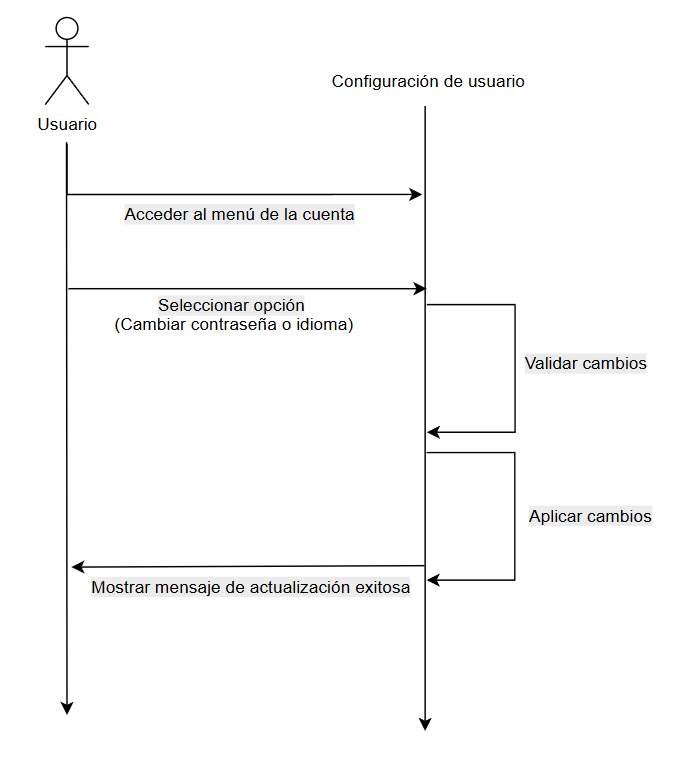
\includegraphics[width=0.8\textwidth]{img/DiagramaCU2.png}
\caption{Diagrama del caso de uso CU2}
\label{fig:DiagramaCU2}
\end{figure}

\subsection*{CU3 - Introducción y validación de URLs de repositorios}

Este caso de uso permite al usuario introducir una o más URLs de repositorios GitHub para su posterior análisis. El sistema se encarga de validar tanto la estructura como el acceso. La figura~\ref{fig:DiagramaCU3-CU6-CU7} describe un flujo de introducción y validación de URLs de repositorios para su posterior visualización.

\textbf{Pasos que sigue el CU:}
\begin{enumerate}
  \item El usuario introduce una o varias URLs.
  \item El sistema valida su formato y accesibilidad.
  \item Si las URLs no son correctamente validadas saltará un mensaje de error. En caso contrario, el análisis se iniciará cuando el usuario pulse el botón..
\end{enumerate}

\subsection*{CU4 - Configuración del análisis de repositorios}

Este caso de uso permite definir cómo se analizarán los datos de los repositorios previamente introducidos. El usuario puede personalizar fechas, tipos de intervalos y métricas. Cada paso incluye validaciones, y al final se habilita la opción de comparar (ver figura~\ref{fig:DiagramaCU4}).

\textbf{Pasos que sigue el CU:}
\begin{enumerate}
  \item El usuario elige el número de días sobre el cual se basarán las medidas de calidad que reflejan medias estadísticas.
  \item El usuario elige entre analizar los repositorios al completo o por intervalos de tiempo.
  \item El usuario elige en qué intervalos de tiempo realizar el análisis.
  \item Se validan las entradas y se habilita el botón \textit{Comparar}.
\end{enumerate}

\begin{figure}[H]
\centering
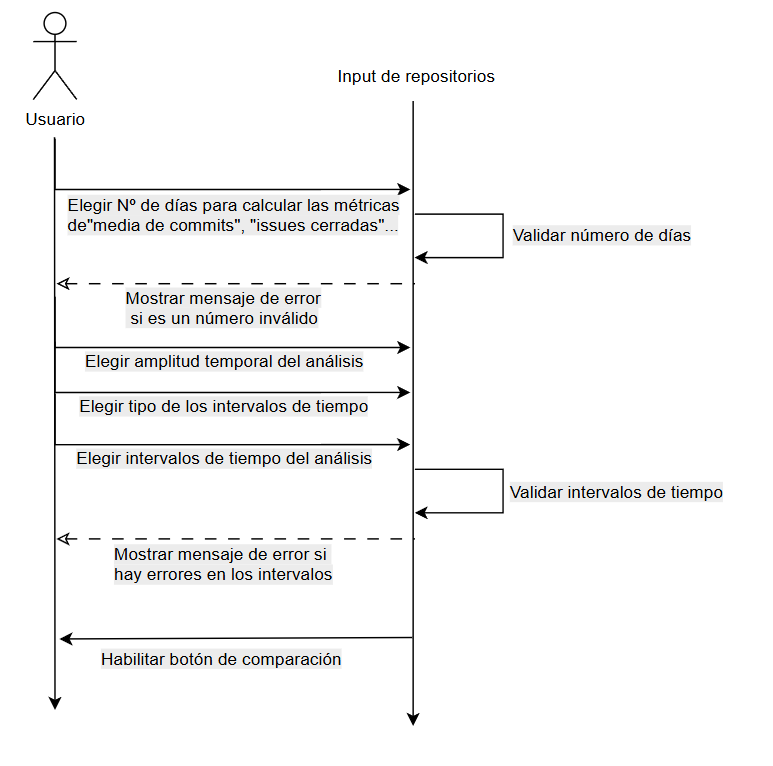
\includegraphics[width=0.8\textwidth]{img/DiagramaCU4.png}
\caption{Diagrama del caso de uso CU4}
\label{fig:DiagramaCU4}
\end{figure}

\subsection*{CU5 - Gestión de grupos de repositorios de referencia}

Este caso de uso permite gestionar grupos de repositorios previamente guardados como referencia comparativa. El usuario puede cargarlos o eliminarlos, siempre y cuando tenga al menos un grupo guardado. (Ver figura~\ref{fig:DiagramaCU5})

\textbf{Pasos que sigue el CU:}
\begin{enumerate}
  \item El usuario accede a la gestión de grupos de repositorios.
  \item Selecciona uno para cargarlo.
  \item Opcionalmente elimina uno o más grupos.
\end{enumerate}

\begin{figure}[H]
\centering
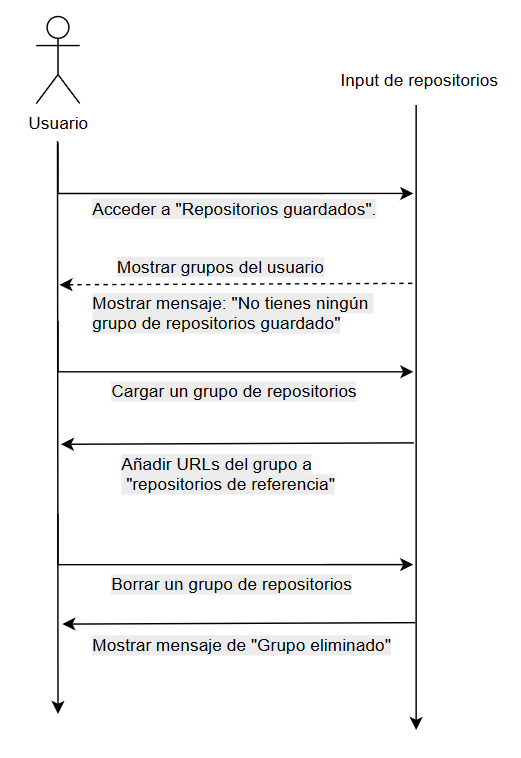
\includegraphics[width=0.8\textwidth]{img/DiagramaCU5.png}
\caption{Diagrama del caso de uso CU5}
\label{fig:DiagramaCU5}
\end{figure}

\subsection*{CU6 - Visualización de prácticas ágiles}

Permite al usuario visualizar los resultados de un análisis automático de prácticas ágiles basado en las medidas de calidad de proceso extraídas de los repositorios. Se presentan los resultados en forma gráfica y textual, indicando qué prácticas se cumplen, en qué medida, y en qué aspectos hay lugar para mejoras. Esto puede observarse en la figura~\ref{fig:DiagramaCU3-CU6-CU7}, junto a la posibilidad de que el usuario cambie de pantalla y vuelva a la de este caso de uso o pase a la del CU7.

\textbf{Pasos que sigue el CU:}
\begin{enumerate}
  \item El sistema muestra los resultados del uso de prácticas ágiles del análisis en forma gráfica y textual.
  \item El usuario revisa qué prácticas de agilidad se cumplen, cuáles no, y los motivos.
\end{enumerate}

\subsection*{CU7 - Comparación de medidas de calidad de proceso}

Este caso de uso permite al usuario comparar visualmente las métricas de calidad de su repositorio analizado con aquellas de uno o más repositorios de referencia previamente cargados. El sistema genera listas comparativas para facilitar la interpretación. Esta funcionalidad, junto a las de los casos de uso CU3 y CU6 se detalla gráficamente en la figura~\ref{fig:DiagramaCU7} siguiendo un flujo detallado del proceso de validación de URLs de repositorios para después ver los resultados.

\textbf{Pasos que sigue el CU:}
\begin{enumerate}
  \item El usuario accede a la sección de comparación.
  \item El sistema genera y muestra listas comparativas con las métricas seleccionadas del repositorio actual y los de referencia.
  \item El usuario analiza los resultados para evaluar el estado de su proyecto.
\end{enumerate}

\begin{figure}[H]
\centering
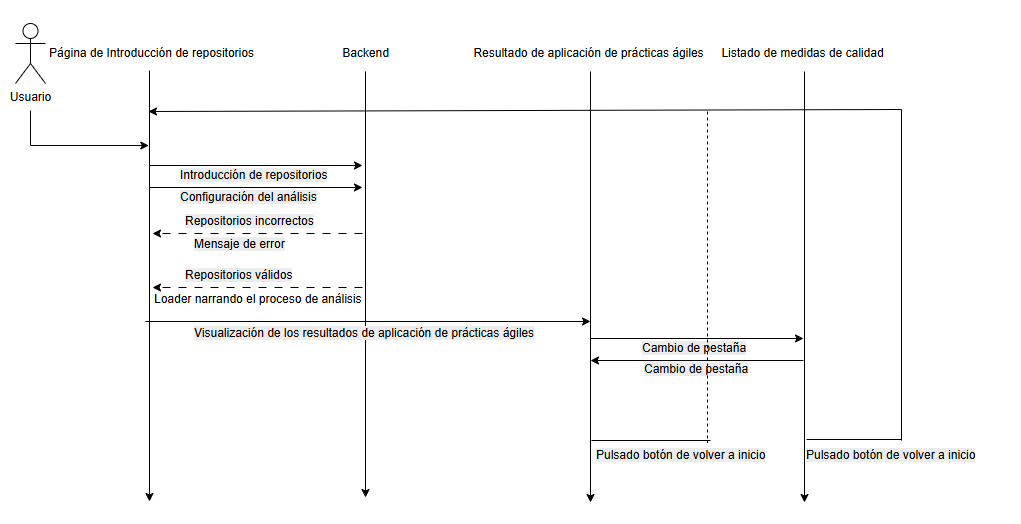
\includegraphics[width=0.8\textwidth]{img/DiagramaCU3-CU6-CU7.png}
\caption{Diagrama del caso de uso CU7}
\label{fig:DiagramaCU3-CU6-CU7}
\end{figure}
\apendice{Documentación técnica de programación}

\section{Introducción}

Este apartado del anexo detalla una guía técnica completa orientada a desarolladores software que quieran trabajar o utilizar la aplicación de Asistente de prácticas ágiles para repositorios en GitHub. Se incluye una guía para clonar el entorno de desarrollo, compilar y ejecutar la aplicación, detallando los pasos necesarios a realizar en la configuración del proyecto para lograrlo.

\section{Estructura de directorios}
A continuación se detalla la estructura de ficheros de todo el proyecto, incluyendo tanto el código fuente de la aplicación desarrollada como la documentación, y readmes.
\begin{itemize}
	
	\item \textbf{/}: Directorio raíz. Contiene el resto de directorios, junto al fichero gitignore y el fichero readme.d principal del proyecto.
	
    \item \textbf{/Memoria/}: Directorio que contiene la documentación del proyecto. En su interior se encuentran:

    \begin{itemize}
        \item Directorio tex/ con los archivos \LaTeX{} que componen la memoria principal y el anexo.
        \item Contiene el fichero \LaTeX{} principal de la memoria y el fichero \LaTeX{} principal del anexo
        \item Ficheros PDF generados correspondientes a la memoria y al anexo.
        \item Carpeta /img con las imágenes utilizadas en los documentos.
        \item Un archivo \texttt{.gitignore} específico para esta carpeta.
        \item Un fichero \texttt{README.md} con información sobre la plantilla utilizada para redactar la documentación.
    \end{itemize}
    
    \item \textbf{/src/}: Carpeta principal que contiene el código fuente de la aplicación web desarrollada. Dentro de este directorio se encuentran:
    
    \begin{itemize}
          \item La carpeta \texttt{frontend/}, que contiene el código de la interfaz de usuario.
          \item La carpeta \texttt{backend/}, que incluye la lógica de servidor y la API, y los modelos de las tablas de la base de datos.
          \item Una copia de la carpeta \texttt{node\_modules/} con las dependencias necesarias.
          \item Un archivo \texttt{README.md} que proporciona una guía sobre la organización del código y cómo distinguir entre el backend y el frontend.
        \end{itemize}
    	
    \end{itemize}

\section{Manual del programador}

Esta sección tiene el objetivo de ser utilizada por desarrolladores de software, programadores o personas interesadas en trabajar en el proyecto para guiar a los mismos a la hora de configurar el entorno de desarrollo y compilar y ejecutar el código fuente para poder probar el mismo. Para ello se numeran los siguientes puntos a tener en cuenta.

\subsection{Entorno de desarrollo}

Para configurar el entorno de desarrollo del proyecto, se sugiere utilizar las herramientas listadas a continuación:

\begin{itemize}
	\item \textbf{Visual Studio Code:} Se trata de un editor de código fuente gratuito, ligero y versátil. Es una herramienta útil para escribir, editar, depurar y gestionar código en una amplia variedad de lenguajes de programación. Se caracteriza por su flexibilidad, extensibilidad y capacidad para integrarse con diversas herramientas y extensiones. 
	\item \textbf{Copilot (Opcional):} Es una extensión de \textit{Visual Studio Code} que asiste al programador con una inteligencia artificial a través de sugerencias de código, lo que acelera mucho el proceso de desarrollo.
	\item \textbf{MongoDBCompass:} Una aplicación de escritorio desde la cual gestionar la conexión y contenidos de la base de datos ubicada en \textbf{Mongo DB Atlas}.
    \item \textbf{GitHubDesktop:} Un entorno gráfico de GitHub de gran utilidad gracias a la infromación visual que brinda sobre los ficheros del repositorio modificados, añadidos o borrados. Ofrece una gran ayuda para hacer \textit{commits}, \textit{pull requests} y \textit{merges} de calidad.
\end{itemize}

\subsection{Obtención del código fuente}

El código fuente del proyecto está disponible en el repositorio en GitHub \url{https://github.com/lod1004/GII-TFG-Asistente-de-practicas-agiles-para-repositorios-en-GitHub}. Es necesario clonar el proyecto para trabajar en él de forma activa. A continuación se describen dos formas para lograrlo:

\begin{itemize}
    \item Descargar e instalar \textbf{GitHub Desktop} desde \url{https://desktop.github.com/} si se prefiere clonar el proyecto gráficamente.

	\item Clonar el repositorio del proyecto desde GitHub de una de las siguientes formas:
	\begin{itemize}
		\item \textbf{Opción 1 - Gráfica (recomendada para usuarios sin experiencia con Git):} Abrir GitHub Desktop, hacer clic en \textit{"File > Clone repository"}, pegar la URL del repositorio y elegir una ubicación en el disco local.
		\item \textbf{Opción 2 - Terminal:} Ejecutar \texttt{git clone \textit{URL-del-repositorio}} en una terminal ubicada en la carpeta donde se desea clonar el repositorio.
	\end{itemize}
\end{itemize}

\subsubsection{Pasos para configurar el entorno}

Una vez clonado el repositorio en una carpeta local, para instalar y configurar el entorno del proyecto correctamente se recomienda seguir los pasos numerados a continuación:

\begin{enumerate}

	\item Descargar e instalar \textbf{Visual Studio Code} desde \url{https://code.visualstudio.com/}.

	\item Descargar e instalar \textbf{Node.js} desde \url{https://nodejs.org/en/download}. Se recomienda la versión LTS más reciente.

	\item Instalar Angular CLI ejecutando en una terminal uno de los siguientes comandos:
	\begin{itemize}
		\item De forma global: \textbf{npm install -g @angular/cli@19.2.3}
		\item O bien, de forma local en la carpeta del proyecto: \textbf{npm install @angular/cli@19.2.3}
	\end{itemize}

    \item Descargar e instalar \textbf{MongoDB Compass} desde \url{https://www.mongodb.com/products/compass}, para visualizar y gestionar la base de datos de forma gráfica.

\end{enumerate}

Además del entorno base, Visual Studio Code permite instalar algunas extensiones que pueden facilitar significativamente el desarrollo, mejorar la productividad y proporcionar soporte inteligente durante la programación. Una de las más destacadas es la ya mencionada extensión de Copilot, una extensión basada en inteligencia artificial que sugiere automáticamente líneas completas de código y funciones enteras a partir del contexto del proyecto y de los comentarios escritos por el programador. Esto resulta especialmente útil en entornos colaborativos o cuando se trabaja con estructuras repetitivas. También se sugiere instalar extensiones como ESLint, que ayuda a mantener un estilo de código coherente y libre de errores comunes, Prettier para el formateo automático del código, y Angular Language Service, que proporciona autocompletado y detección de errores específicos de Angular en tiempo real. Para entornos backend con Node.js y MongoDB, extensiones como MongoDB for VS Code permiten realizar consultas directamente desde el editor y visualizar colecciones, lo cual es muy conveniente durante el desarrollo y depuración. Estas herramientas integradas en el editor permiten una experiencia de desarrollo más fluida, profesional y eficiente.

\section{Compilación, instalación y ejecución del proyecto}
\label{sec:compilacion}

Una vez configurado el entorno del proyecto y los sercios externos, se detallan los siguientes pasos a seguir necesarios para compilar e instalar lo necesario para poder ejecutar la aplicación.

\begin{enumerate}

	\item Desde la raíz del repositorio clonado, navegar a la carpeta \textbf{src/backend} y ejecutar los siguientes comandos en una terminal:
	\begin{itemize}
		\item \textbf{npm install} para instalar las dependencias del servidor.
		\item En el fichero .env del back se debe incluir una token de GitHub para poder hacer las peticiones a través de la API. Se puede ver más información sobre las token de GitHub en el siguiente enlace: \url{https://docs.github.com/en/authentication/keeping-your-account-and-data-secure/managing-your-personal-access-tokens}. 
        \item También puede ser necesario añadir una conexión de MongoDB Atlas o, en su defecto, dejar la que ya está y usar la base de datos existente.
		\item Ejecutar el backend con \textbf{npm run dev} o \textbf{node server.js}, según lo especificado en la documentación del proyecto.
	\end{itemize}

	\item En una nueva terminal, navegar a \textbf{src/frontend} y ejecutar:
	\begin{itemize}
		\item \textbf{npm install} para instalar las dependencias del cliente.
		\item \textbf{ng serve -o} para iniciar la aplicación Angular en el navegador y que la pestaña se abra de forma automática.
        \item \textbf{Importante} asegurarse de que los servicios del frontEnd (AuthService y RepositoryService) utilicen el environment correcto. ('../../environments/environment' para ejecutar en local o '../../environments/environment.prod' para acceder al BAckend subido en el despliegue continuo en \textbf{React})
	\end{itemize}
\end{enumerate}

\section{Pruebas del sistema}

El sistema fue sometido a diversas pruebas para garantizar su correcto funcionamiento, mayoritariamente manuales, por parte del autor, tutor, y usuarios externos. Debido a la ventaja de división de código en componentes de Angular, la mayoría de cambios de la aplicación eran añadidos al código, y rara vez modificaban lo hecho previamente, lo que ahorró mucho tiempo de pruebas. SIn embargo, hay dos tipos de pruebas relevantes que se hicieron durante el desarrollo del sistema.

\subsection{Prueba general del sistema}

La prueba general principal usada para comprobar el funcionamiento completo del sistema fue la de comparar un repositorio consigo mismo. Esta prueba garantiza que tanto la recopilación de métricas como la lógica de comparación funcionan de forma coherente.

Según la lógica interna de la aplicación, al comparar un repositorio consigo mismo en los mismos intervalos de tiempo, se espera que los resultados se comporten de la siguiente forma:

\begin{itemize}
    \item Las medidas de calidad de proceso deben ser idénticas en ambos repositorios, dado que se trata del mismo repositorio y el análisis se realiza bajo las mismas condiciones y fechas.
    
    \item En la evaluación de prácticas ágiles, todas las medidas que sean aplicables deben considerarse superadas, ya que no hay diferencias entre los repositorios comparados. Las únicas medidas que podrían no superarse son aquellas que no se aplican al repositorio (por ejemplo, por falta de datos), ya que estas se contabilizan como "no completadas", incluso si en el repositorio comparado tampoco se aplican.
\end{itemize}

Esta prueba es útil no solo para verificar que el sistema se comporta como se espera en condiciones ideales, sino también para validar la integridad de los datos obtenidos desde GitHub, el cálculo de métricas y la aplicación de las reglas de evaluación automatizadas.

\subsection{Pruebas con SonarCloud}

Además de la lógica interna de evaluación y comparación, el proyecto hace uso de \textbf{SonarCloud}, integrado en el repositorio de GitHub como plataforma de análisis de calidad del código. SonarCloud permite detectar de forma automatizada problemas como errores de seguridad, código duplicado, malas prácticas y código que no sigue los estándares recomendados.

La integración con SonarCloud ha resultado esencial para mantener un código de alta calidad y detectar posibles refactorizaciones necesarias de forma rápida y visual.

Gracias a esta herramienta se ha podido reforzar la seguridad, mantenibilidad y fiabilidad del proyecto, así como evitar la duplicación de código y las posibles vulnerabilidades que puedan surgir durante el proceso de desarrollo software
\apendice{Documentación de usuario}

\section{Introducción}
Este apartado del anexo de Asistente de prácticas ágiles para repositorios en GitHub tiene como objetivo proporcionar a los usuarios las instrucciones necesarias para utilizar la aplicación web desarrollada en el proyecto. 
Está orientado a usuarios que hayan decidido usar la aplicación para evaluar el uso de prácticas ágiles en sus repositorios, así como observar las diferentes medidas de calidad de proceso que puedan ayudar a visualizar el progreso del desarrollo de software.
Se describirán los requisitos recomendados de los usuarios, los pasos para la instalación y, al final, una guía de usuario que explica cómo realizar los distintos casos de uso aprovechando las funcionalidades disponibles en la aplicación.

\section{Requisitos de usuarios}
Para poder utilizar la aplicación web, se requiere del dispositivo del usuario los requisitos listados a continuación:

\subsection*{Permisos requeridos del usuario}
La aplicación web requiere únicamente de acceso a internet para ser utilizada tanto para registrarse e iniciar sesión como para analizar y comparar repositorios.
No se requiere de una dirección de correo electrónico o una cuenta de GitHub para utilizar los servicios de la aplicación, pero se debe tener en cuenta que, aunque los repositorios a analizar deben ser obligatoriamente \textbf{públicos} (lo cual deja a entender que el propietario accede a que se obtenga información del repositorio), se accederá a los contenidos de estos para proceder con la comparación, incluyendo:

\begin{itemize}
    \item \textbf{Información de \textit{issues}:} Número de \textit{issues}, fechas, título, descripción, etiquetas, imágenes, autores y personas asignadas.
    \item \textbf{Información de \textit{commits}:} Número de \textit{commits}, fechas, título, descripción, y autores.
    \item \textbf{Información de \textit{releases}:} Número de \textit{releases} y  \textit{tags}, fechas, título, descripción y autores.
    \item \textbf{Información de \textit{pull requests}:} Número de \textit{pull requests}, fechas, título, descripción, etiquetas, imágenes, autores y personas asignadas.
    \item \textbf{Información de ficheros \textit{workflow} de GitHub Actions:} (Número de ficheros, ejecuciones exitosas y frecuencia de ejecución).
    \item \textbf{Información de los participantes del repositorio:} Nombre de los participantes y su actividad en el repositorio.
\end{itemize}

\subsection*{Requisitos de Hardware recomendados}
\begin{itemize}
	\item Se recomienda utilizar un computador para usar la aplicación, pues está pensada para ser utilizada en entornos de desarrollo de software, por lo que no se sugiere acceder desde un dispositivo móvil.
	\item Sistema operativo funcional con navegadores web (Firefox, Google Chrome, Opera, etc).
\end{itemize}

\section{Instalación}

Debido al despliegue continuo de la aplicación web, no es necesario realizar ninguna instalación para acceder a las funcionalidades de la misma. Basta con acceder a la siguiente URL con el despliegue final de la aplicación: \textbf{\url{https://gii-tfg-asistente-de-practicas-agiles-para-repositor-f3z9mn3lt.vercel.app/}}

En caso de querer configurar, instalar y ejecutar el código fuente en formato local, se dispone de una explicación detallada por pasos en el apartado anterior de este documento.

\section{Manual del Usuario}
En esta sección se detallan todas las funcionalidades disponibles en la aplicación paso por paso para ser utilizadas por los usuarios de manera efectiva.

\subsection{Creación y acceso a la cuenta}

Permite al usuario crear una cuenta mediante la opción de registro y acceder a la aplicación mediante inicio de sesión.

\begin{figure}[H]
\centering
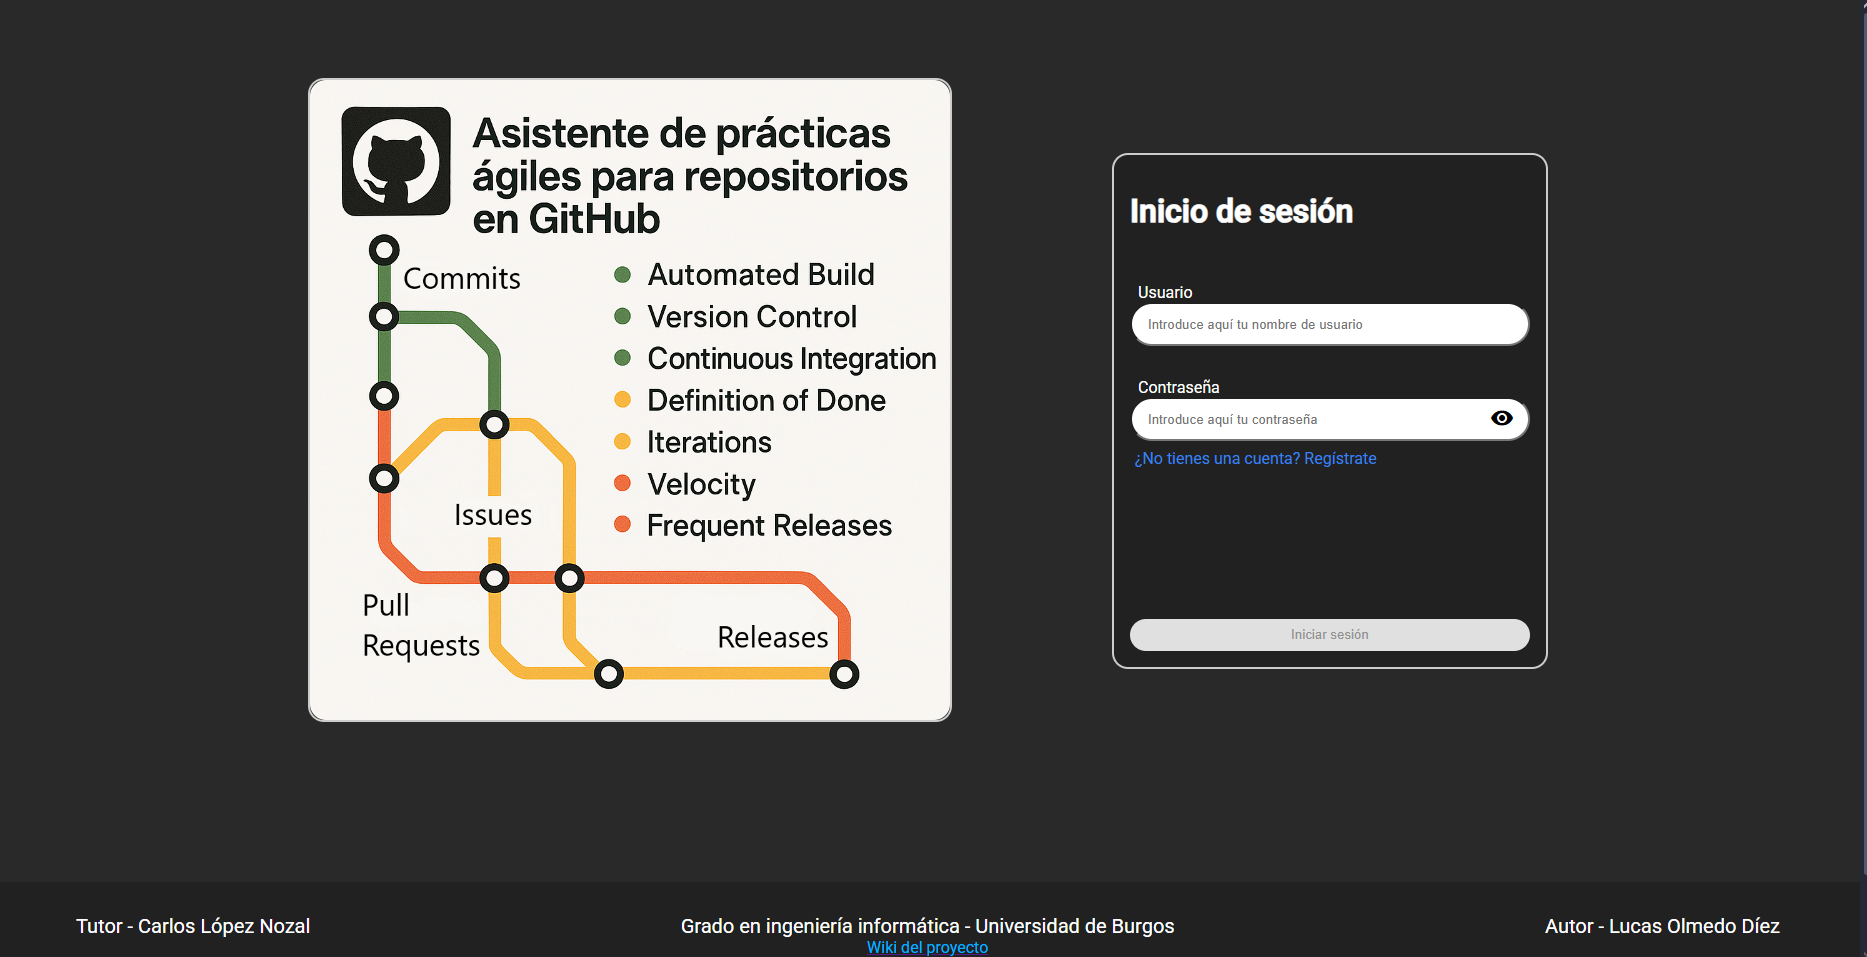
\includegraphics[width=0.8\textwidth]{img/E1-login.png}
\caption{Inicio de sesión del usuario}
\label{fig:E1-login}
\end{figure}

\begin{figure}[H]
\centering
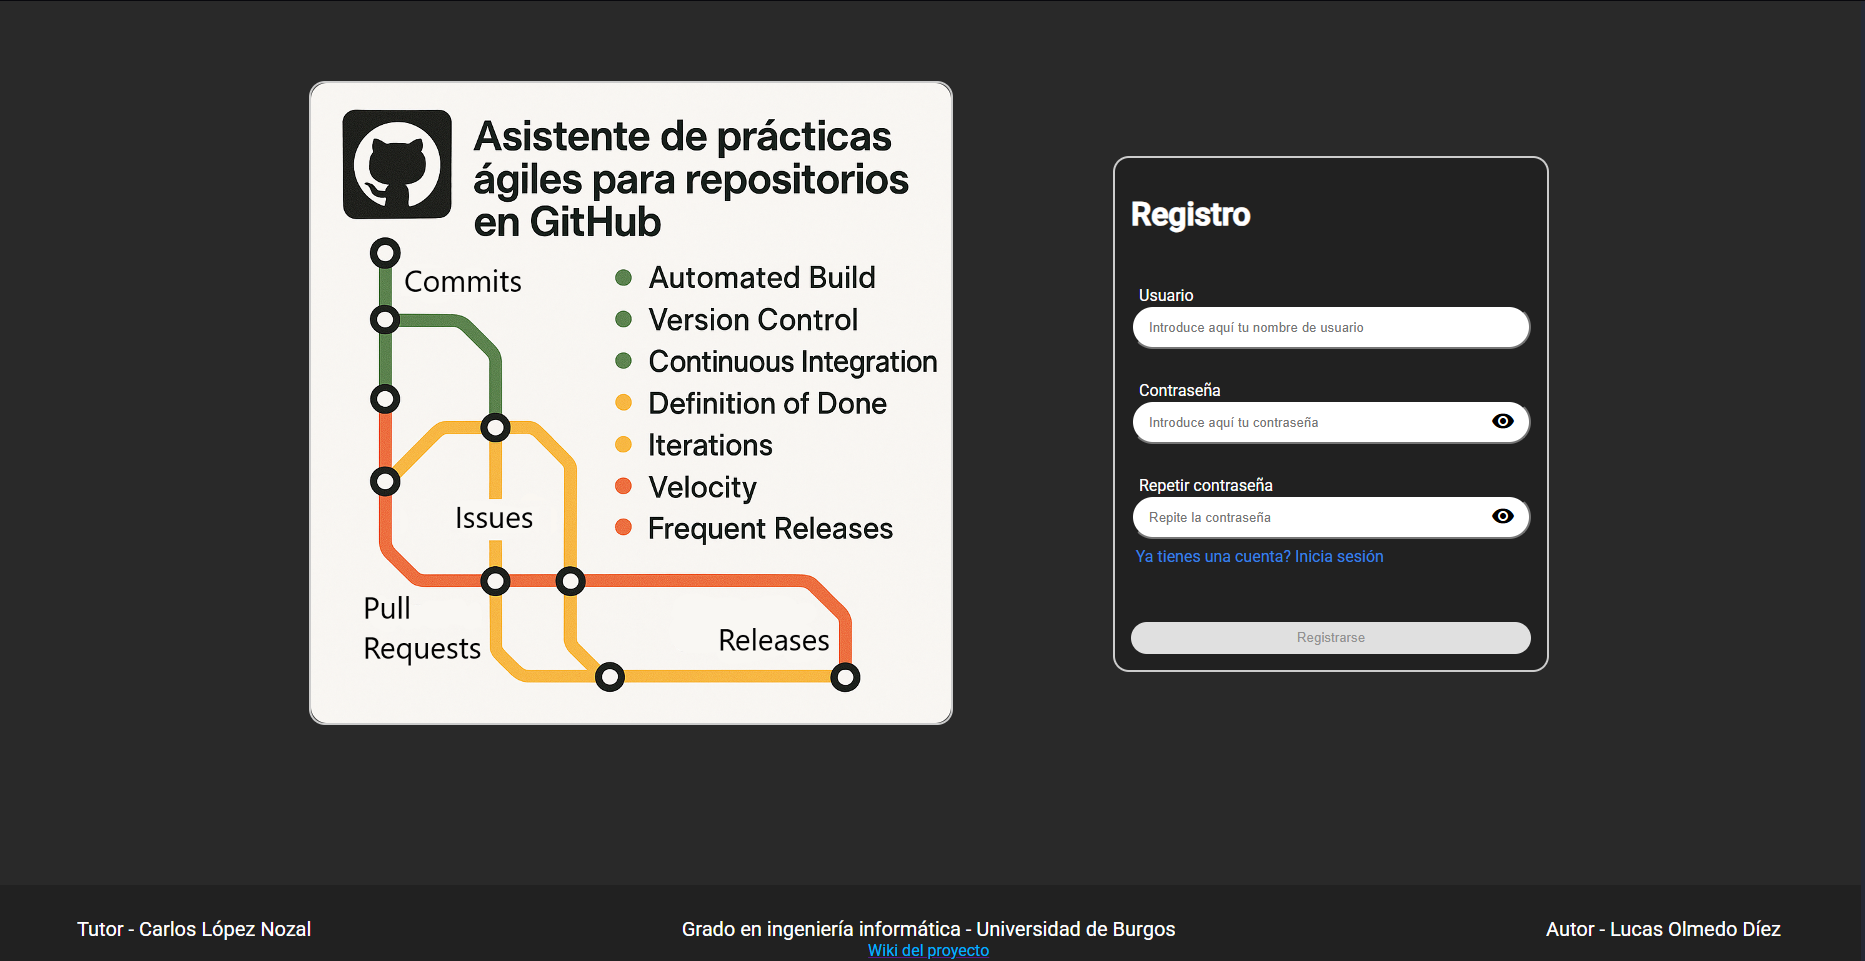
\includegraphics[width=0.8\textwidth]{img/E2-register.png}
\caption{Registro del usuario}
\label{fig:E2-register}
\end{figure}

\begin{itemize}
    \item El usuario accede a la página de registro o inicio de sesión.
    \item El usuario introduce los datos necesarios (usuario y contraseña).
    \item El sistema verifica la validez de los datos.
    \item El sistema registra al usuario o permite el acceso según corresponda.
\end{itemize}

\newpage
\subsection{Configuración de la cuenta}

Permite al usuario cambiar la contraseña y modificar el idioma de la aplicación.

\begin{figure}[H]
\centering

\includegraphics[width=0.8\textwidth]{img/E3-user-configuration.png}
\caption{Configuración del usuario}
\label{fig:E3-user-configuration}
\end{figure}

\begin{itemize}
    \item El usuario puede cambiar el idioma de la interfaz entre inglés y español mediante el icono de la bandera
    \item El usuario pulsa la opción de cambio de contraseña e introduce los datos necesarios (usuario, contraseña actual y nueva contraseña).
    \item El sistema verifica la validez de los datos.
    \item El sistema cambia la contraseña del usuario e inicia sesión automáticamente.
\end{itemize}

\newpage
\subsection{Introducción y validación de URLs de repositorios}

Permite al usuario introducir URLs de repositorios GitHub y valida su formato y accesibilidad.

\begin{figure}[H]
\centering
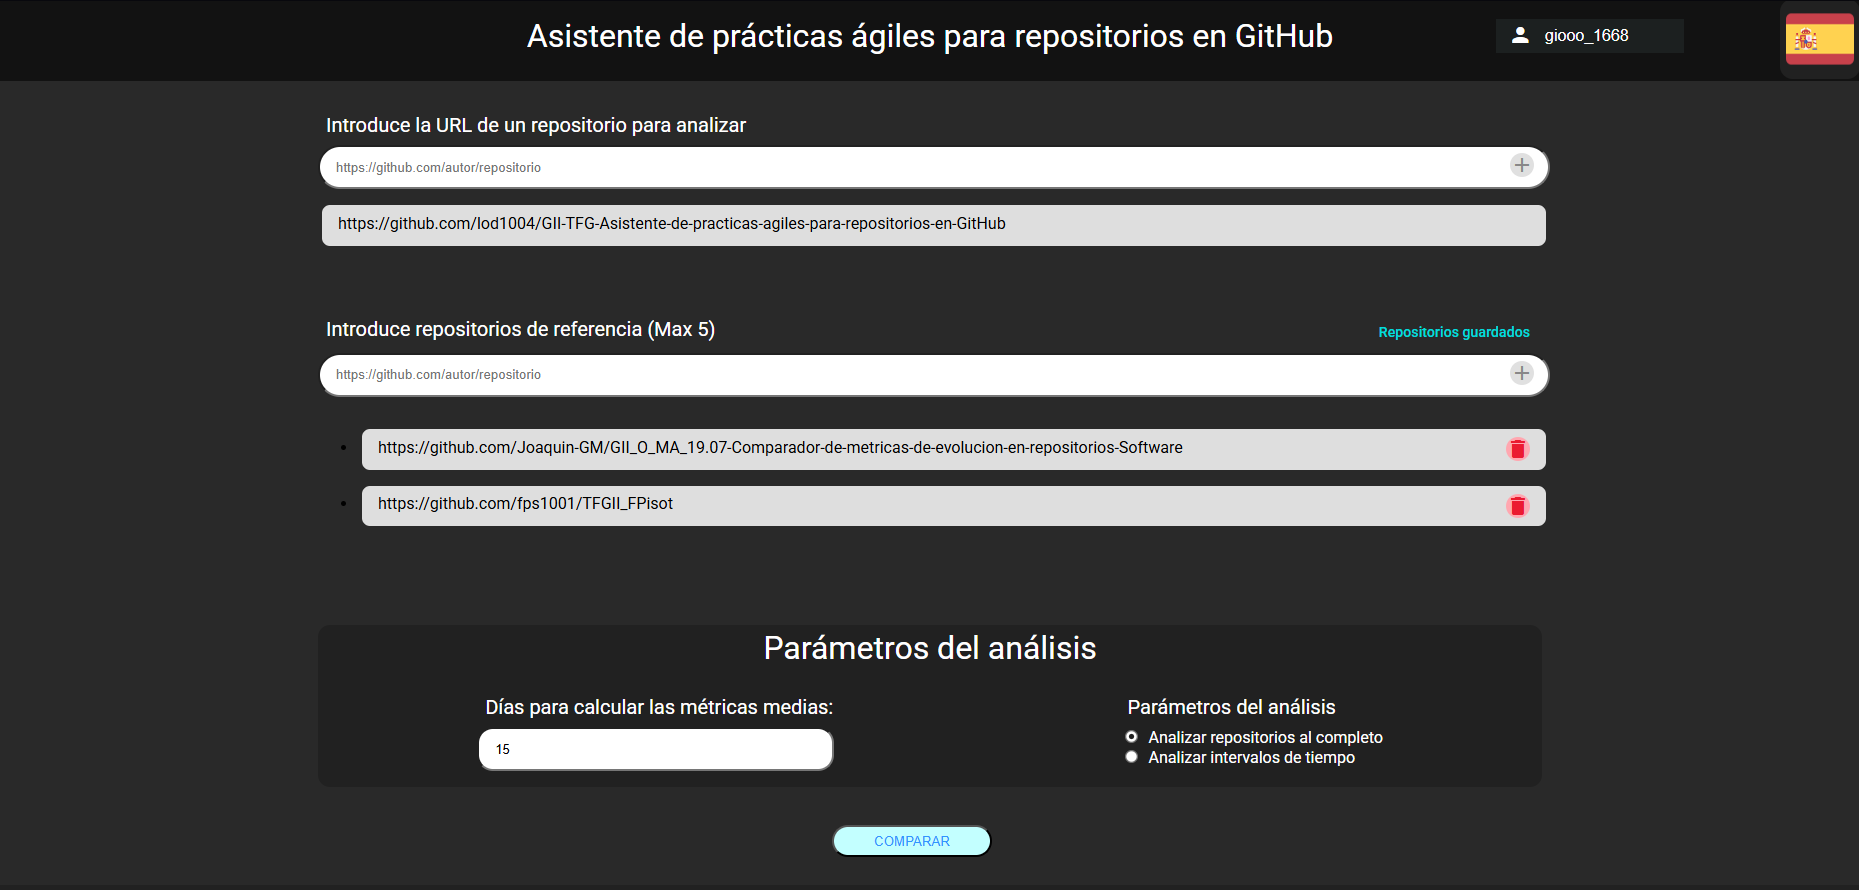
\includegraphics[width=0.8\textwidth]{img/E4-urls.png}
\caption{Validación de URLs de repositorios}
\label{fig:E4-urls}
\end{figure}

\begin{itemize}
    \item El usuario introduce una URL de repositorio a analizar y una o varias URLs de repositorios de referencia.
    \item El sistema valida las urls.
\end{itemize}

\newpage
\subsection{Configuración del análisis de repositorios}

El usuario configura cómo se analizarán los datos del repositorio: número de días para calcular las métricas temporales, análisis completo o por intervalos, usar intervalos absolutos o relativos y los períodos de los intervalos de tiempo del análisis.

\begin{figure}[H]
\centering
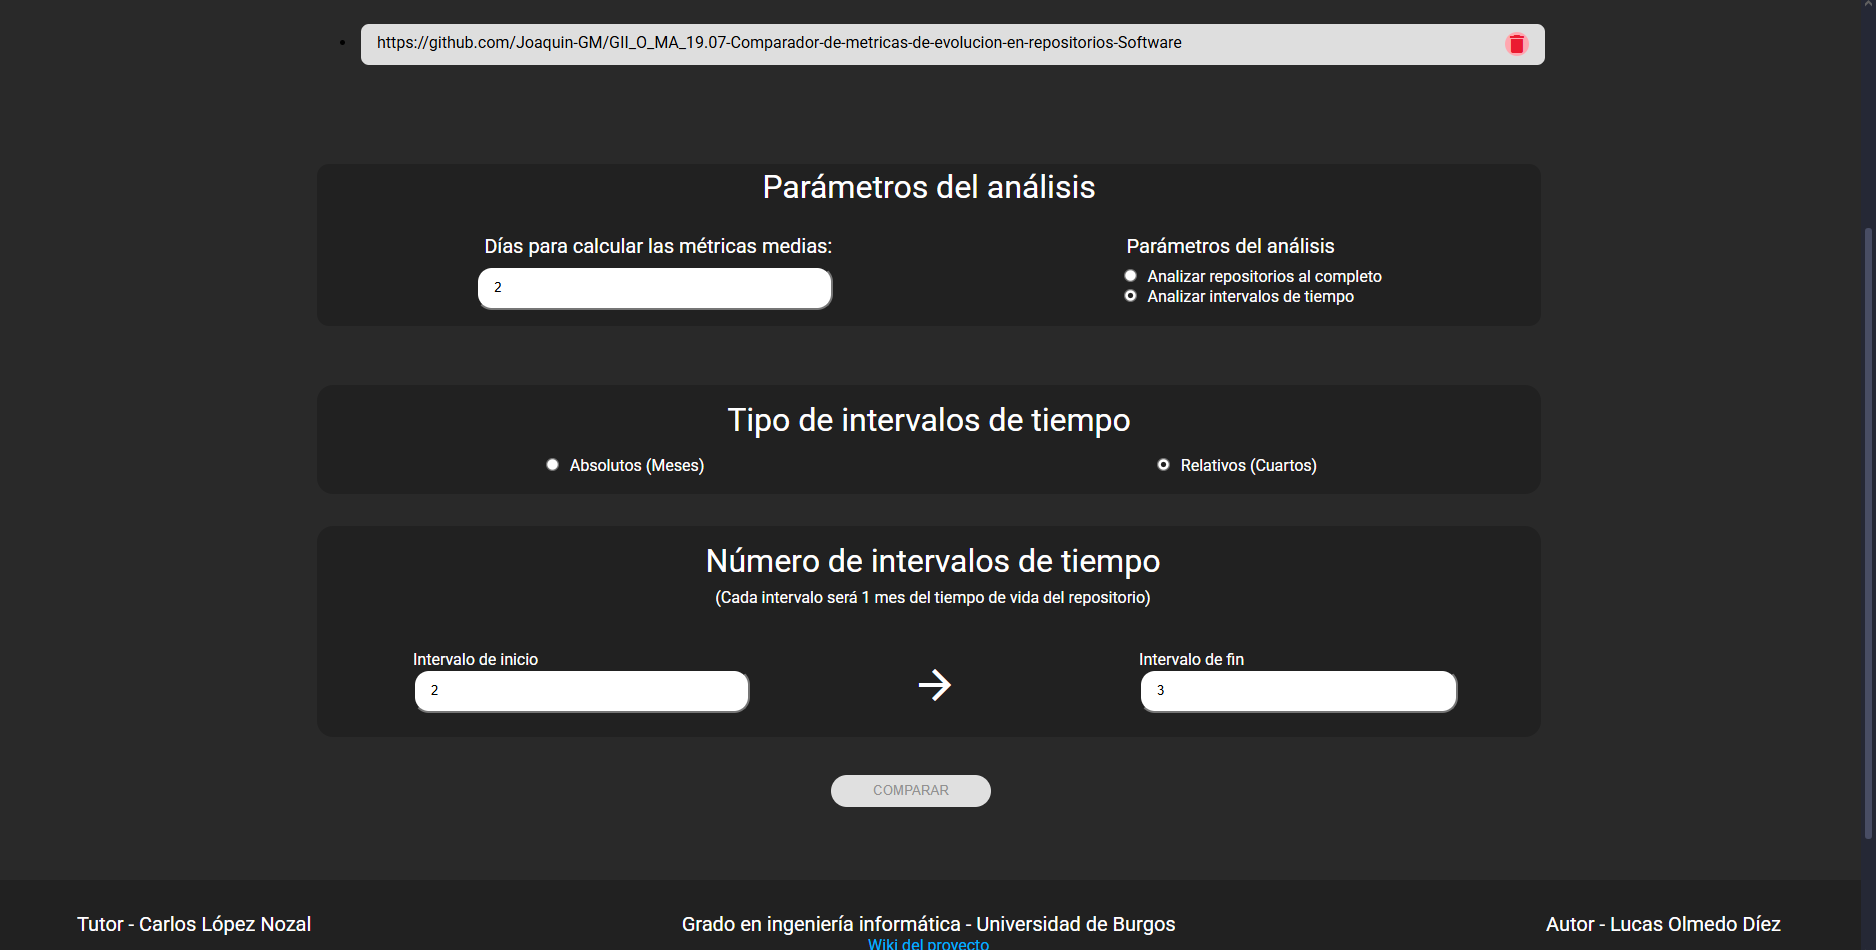
\includegraphics[width=0.8\textwidth]{img/E4.1-configuracion-analisis.png}
\caption{Configuración del análisis de los repositorios}
\label{fig:E4.1-configuracion-analisis}
\end{figure}

\begin{itemize}
    \item El usuario selecciona si analizar los repositorios al completo o analizarlos por intervalos.
    \item Ajusta el número de días para calcular las métricas de medias.
    \item Elige el tipo de intervalos entre absolutos o relativos.
    \item Se eligen los intervalos del análisis.
\end{itemize}

\newpage
\subsection{Gestión de grupos de repositorios de referencia}

Permite al usuario cargar o borrar grupos de repositorios previamente guardados para usarlos como referencia comparativa en los análisis.

\begin{figure}[H]
\centering
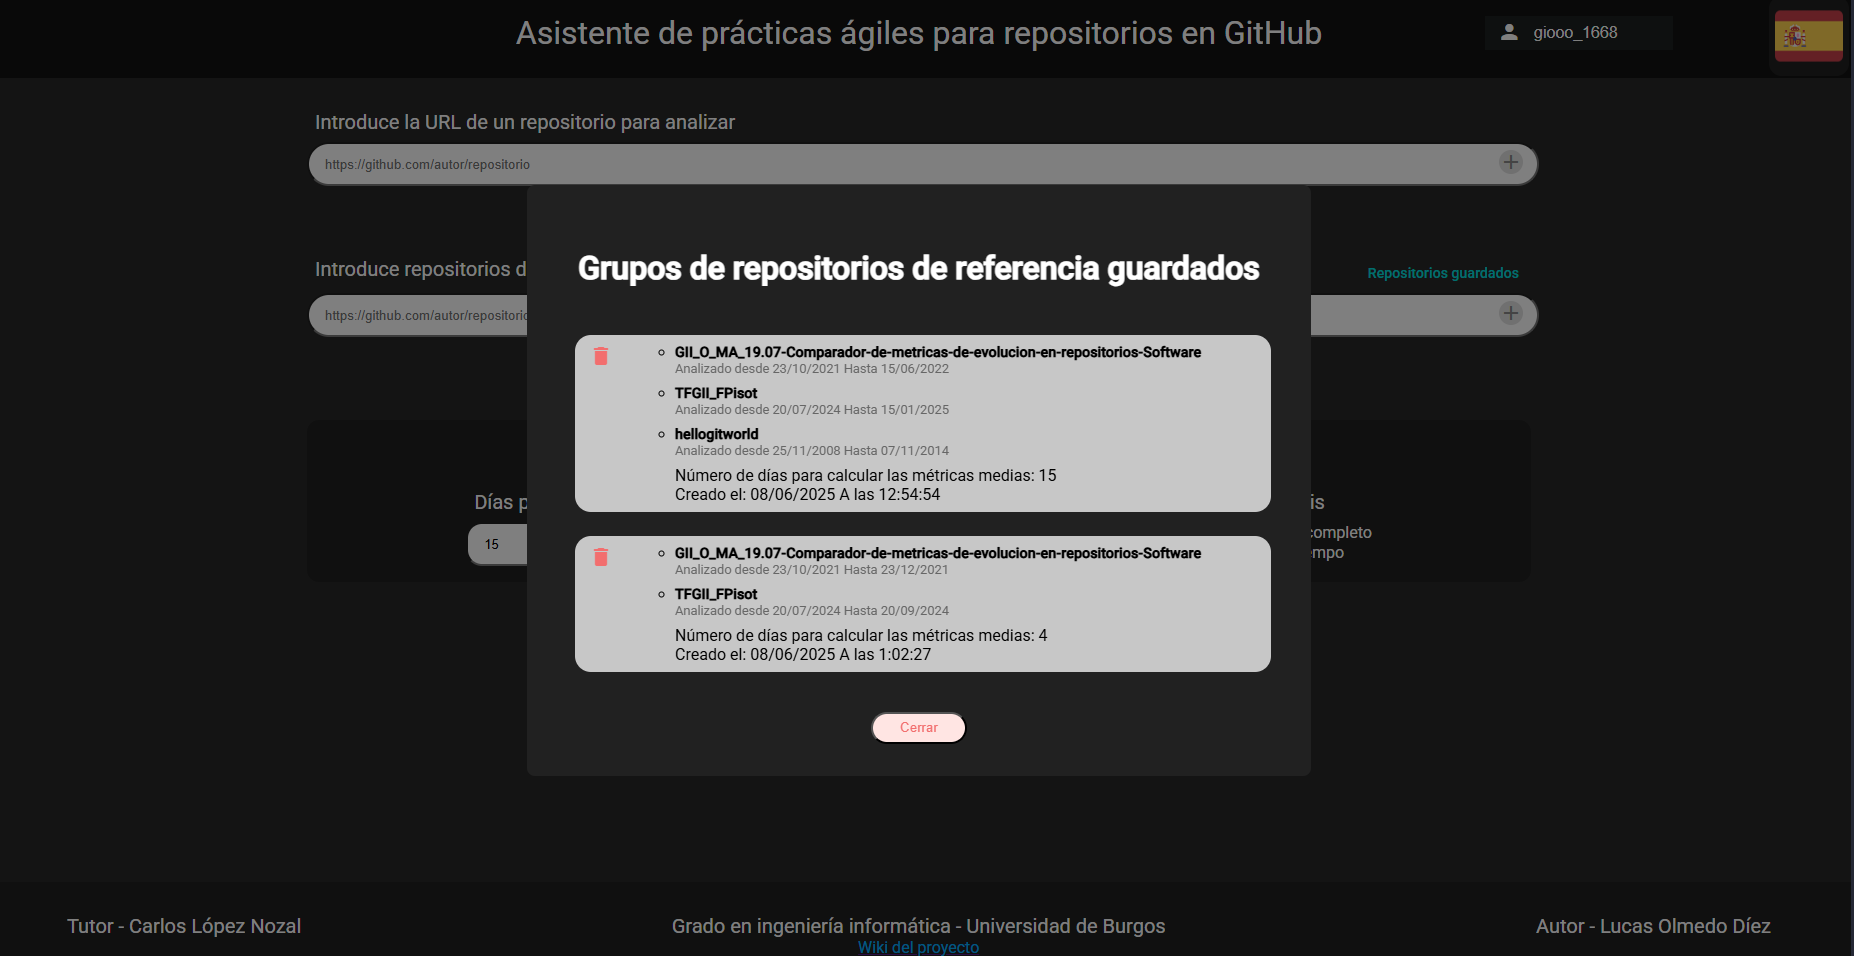
\includegraphics[width=0.8\textwidth]{img/E5-grupos.png}
\caption{Gestión de grupos de repositorios}
\label{fig:E5-grupos}
\end{figure}

\begin{itemize}
    \item El usuario accede a la sección de gestión de repositorios guardados.
    \item Selecciona un grupo de repositorios guardado previamente y lo carga.
    \item (Opcional) Elimina uno o más grupos guardados si lo desea.
\end{itemize}

\newpage
\subsection{Visualización de prácticas ágiles}

Permite al usuario visualizar el grado de adopción de buenas prácticas ágiles evaluadas automáticamente por el sistema a partir de los datos del repositorio.

\begin{figure}[H]
\centering
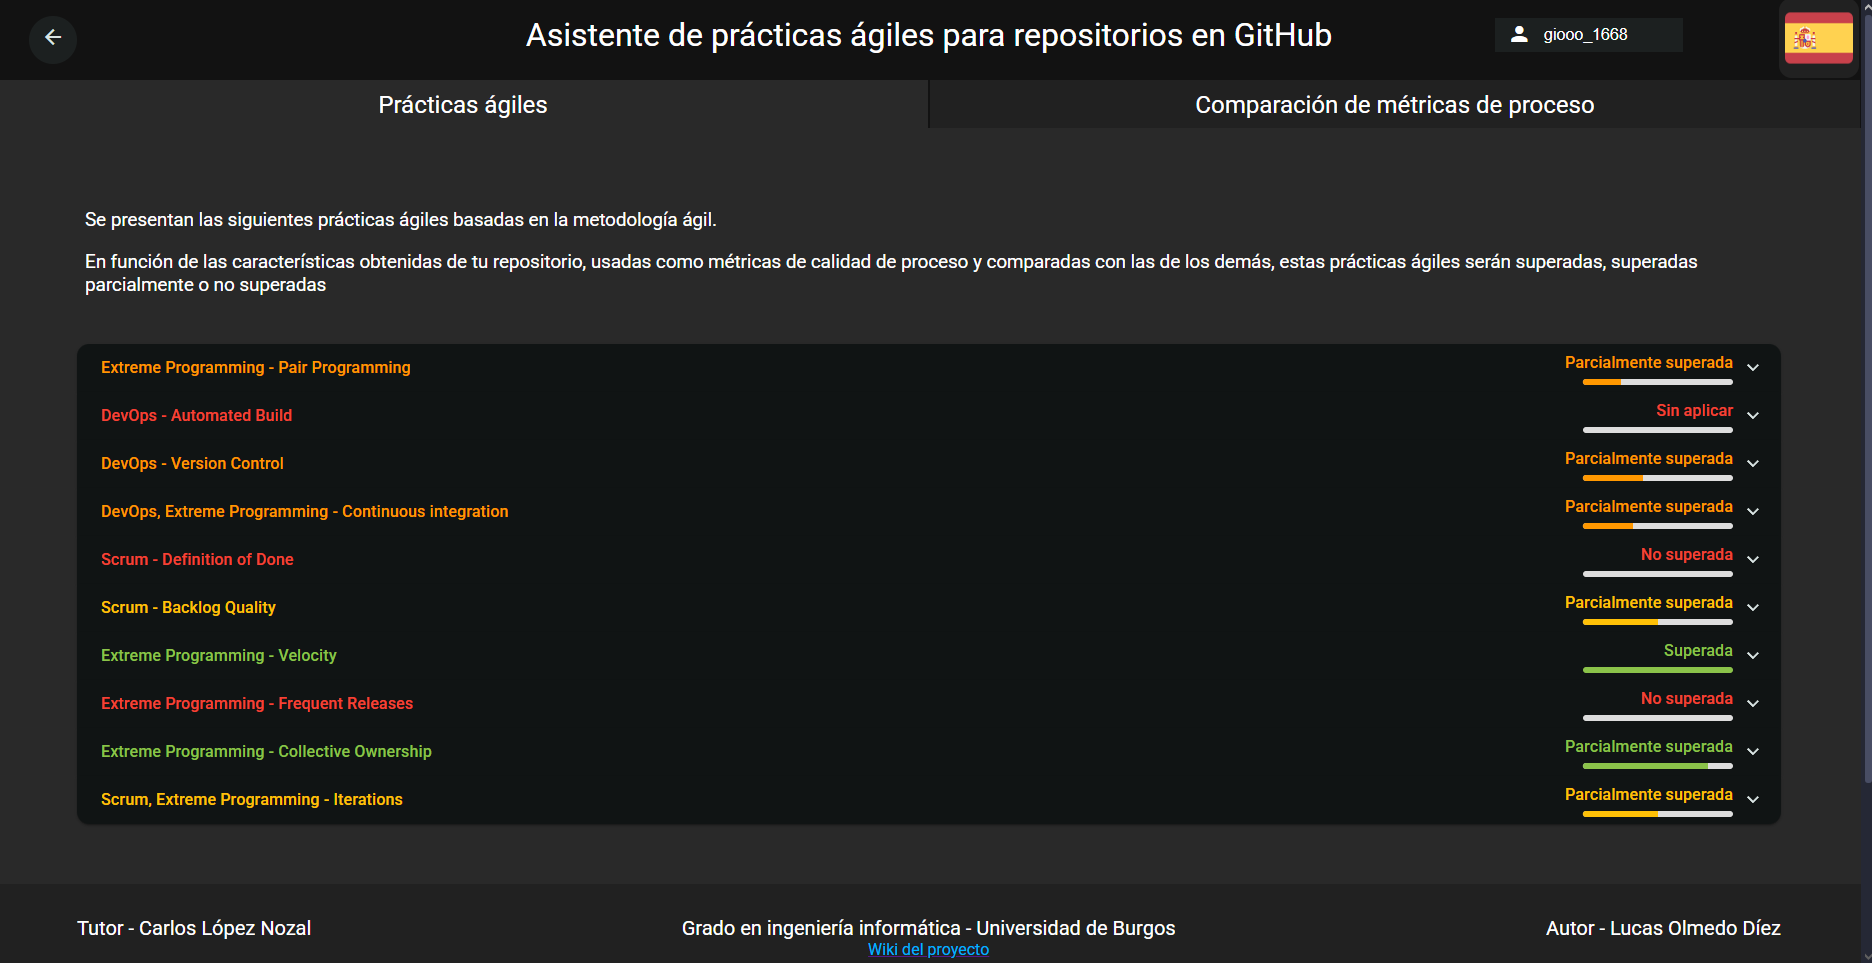
\includegraphics[width=0.8\textwidth]{img/E6-practicas-agiles.png}
\caption{Evaluación de buenas prácticas ágiles}
\label{fig:E6-practicas-agiles}
\end{figure}

\begin{figure}[H]
\centering
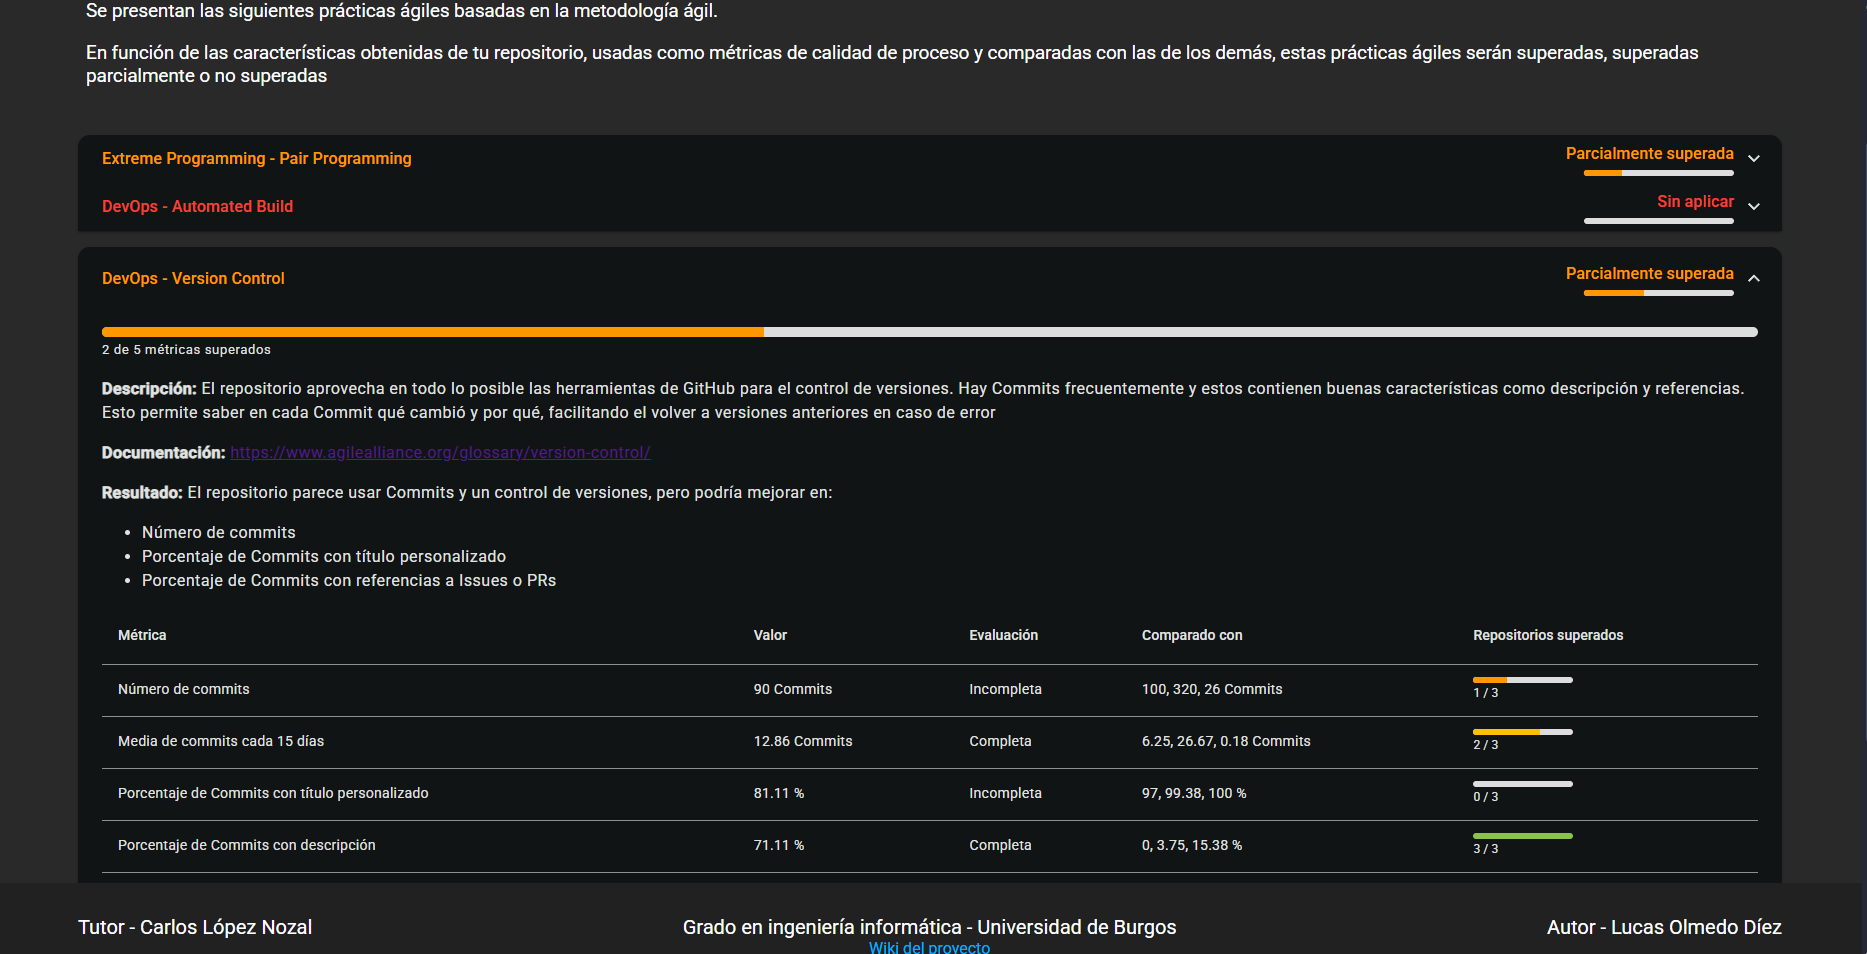
\includegraphics[width=0.8\textwidth]{img/E6.1-detalle-practicas-agiles.png}
\caption{E6: Detalle de las prácticas ágiles}
\label{fig:E6.1-detalle-practicas-agiles}
\end{figure}

\begin{itemize}
    \item El sistema muestra los resultados del análisis de buenas prácticas en formato gráfico y textual.
    \item El usuario puede seleccionar cada práctica ágil para ver los detalles de su evaluación y comparación entre repositorios.
\end{itemize}

\newpage
\subsection{Comparación de medidas de calidad de proceso}

Permite comparar visualmente las métricas del repositorio analizado con las de los repositorios de referencia cargados.

\begin{figure}[H]
\centering
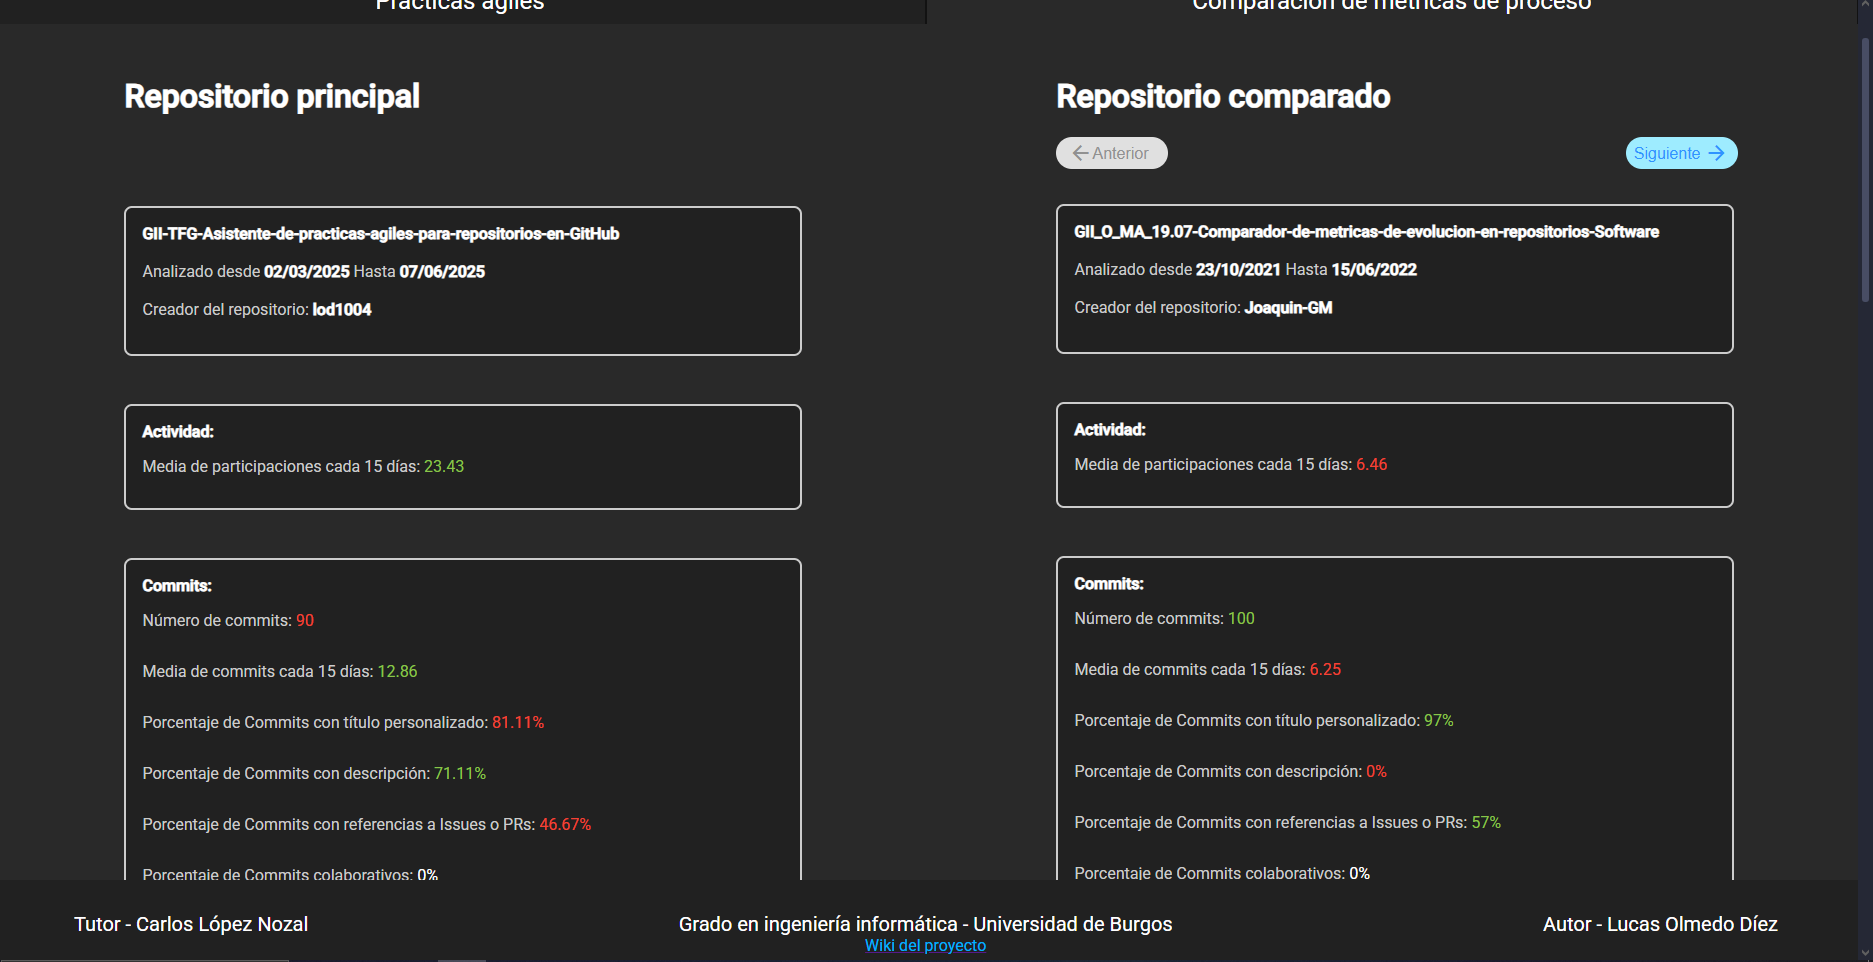
\includegraphics[width=0.8\textwidth]{img/E7-metricas.png}
\caption{Comparación con repositorios de referencia}
\label{fig:E7-metricas}
\end{figure}

\begin{itemize}
    \item El usuario accede a la sección de comparación.
    \item El sistema genera y muestra listas comparativas de las métricas seleccionadas.
    \item El usuario puede elegir qué repositorio de referencia mostrar para compararlo.
\end{itemize}

\apendice{Anexo de sostenibilización curricular}

\section{Introducción}
Durante el desarrollo de este TFG, centrado en la creación de una aplicación web para el análisis automatizado de prácticas ágiles y métricas de calidad de proceso en proyectos alojados en GitHub, he aplicado diversas competencias de sostenibilidad de forma transversal. Este trabajo ha sido una oportunidad para reflexionar sobre cómo el desarrollo software puede contribuir de manera activa al cumplimiento de los Objetivos de Desarrollo Sostenible (\acrfull{ods}).

El análisis del desarrollo software, combinado con el uso de las prácticas ágiles permiten fomentar procesos de mejora continua que reduzcan el desperdicio de recursos humanos y computacionales, a la vez que promueven modelos colaborativos, transparentes y sostenibles. La herramienta desarrollada contribuye a una mayor conciencia en torno a la eficiencia y responsabilidad dentro de los equipos de desarrollo software.

\section{Competencias de Sostenibilidad en el proyecto}

\subsection{F.2.1. Adquisición de conocimiento de competencias de sostenibilidad}
A través de este proyecto, he sido capaz de relacionar el desarrollo tecnológico con los retos globales de sostenibilidad. La aplicación se enfoca en facilitar el análisis reflexivo de proyectos software, lo que permite a los equipos evaluar sus prácticas y alinear sus metodologías con objetivos más amplios como la eficiencia, la justicia laboral (mediante la mejora del clima de equipo), o el acceso equitativo al conocimiento abierto.

\subsection{F.2.2. Sostenibilidad al tomar decisiones de proyecto}
He priorizado el uso eficiente de recursos en la arquitectura del sistema, optando por tecnologías open-source, integraciones ligeras con la API de GitHub para minimizar el consumo energético y computacional. Se evita la persistencia innecesaria de datos, lo que contribuye al uso responsable de almacenamiento y procesamiento en servidores.

\subsection{F.2.3. Fomento de la participación colectiva}
Este trabajo promueve el uso de métricas abiertas y replicables para evaluar proyectos en GitHub, lo que incentiva la participación colaborativa en comunidades de desarrollo software. Al facilitar la evaluación colectiva de buenas prácticas, la herramienta ayuda a fortalecer ecosistemas de software más transparentes, resilientes y responsables.

\subsection{F.2.4. Ética del proyecto}
Durante el desarrollo se ha seguido un enfoque ético que evita la recopilación innecesaria de datos personales, se promueve el análisis de repositorios públicos y se fomenta el uso responsable de la tecnología como instrumento para mejorar la transparencia y la calidad en el trabajo en equipo, sin fomentar modelos competitivos insostenibles o presiones laborales indebidas.

\subsection{F.2.5. Conciencia sobre Sostenibilidad en el Desarrollo Software}
Una parte clave del proyecto ha sido su valor educativo. La herramienta actúa como recurso de concienciación para estudiantes y desarrolladores que buscan mejorar sus prácticas en el desarrollo software y planificación para el mismo. Fomenta la reflexión sobre el ciclo de vida de los proyectos de software, sus tareas y componentes, la calidad de sus procesos y su sostenibilidad a largo plazo.

\section{Conclusión}
El desarrollo de este proyecto ha fortalecido mi comprensión de cómo el software no es únicamente una herramienta técnica, sino un elemento transformador con capacidad de influir en dimensiones sociales y económicas. Aplicar competencias de sostenibilidad en el diseño, implementación y propósito de esta herramienta me ha hecho más consciente de las decisiones éticas y técnicas que tomamos como desarrolladores software. Estoy convencido de que este tipo de soluciones tecnológicas son fundamentales para alcanzar un desarrollo sostenible.


\bibliographystyle{plain}
\bibliography{bibliografiaAnexos}

\end{document}
